%----------------------------------------------------------------------------------------
%	PACKAGES AND OTHER DOCUMENT CONFIGURATIONS
%----------------------------------------------------------------------------------------

\documentclass[12pt,fleqn]{report} % Default font size, left-justified equations, chapters start on any page

%----------------------------------------------------------------------------------------

\input{structure} % Insert the commands.tex file which contains the majority of the structure behind the template
\input{structureSG}


%----------------------------------------------------------------------------------------

\begin{document}

\pageDeGarde

\chapter*{Introduction}

Bienvenue à toutes et à tous en cours de mathématiques ! \\
C’est une année qui sera très riche en connaissances et qui vous apportera des bases en mathématiques pour tout le reste de vos études, notamment si vous souhaitez poursuivre des études scientifiques. \\
C’est pour cette raison que le rythme sera assez soutenu avec la réalisation d’un chapitre par semaine. Ce début d’année sera plutôt calculatoire, il est très important d’être à l’aise en calcul ! Le calcul ne doit pas être un obstacle à votre raisonnement.\\
De plus, les chapitres que nous allons aborder tout au long de cette année ne seront pas indépendants les uns des autres. En effet, les mathématiques forment un tout et des notions du début d’année peuvent vous servir à mieux appréhender les chapitres suivants.\\
Le cours de mathématiques peut être comparé à une série, si on rate un épisode on ne comprend plus la suite ! Il faudra donc vous assurer d’être à jour dans chaque chapitre tout au long de l'année. \\
\subsection*{Objectif}
L'objectif de ce cours est de VOUS permettre de  PROGRESSER. Un bon scientifique doit développer 4 capacités essentielles : \begin{itemize}
	\item \textbf{Puissance de calcul}. Avant de pouvoir comprendre, créer, trouver des solutions il faut que son cerveau puisse traiter, organiser et simplifier les informations rapidement.
	\item \textbf{Finesse de compréhension}. Avant de comprendre, il faut comprendre qu'il y a plusieurs niveaux de compréhension. \\ On peut comprendre plus ou moins finement le fait qu'un pomme tombe au sol.\begin{enumerate}
		\item Compréhension très grossière : La pomme tombe par terre car je le vois.
		\item Compréhension grossière : La pomme tombe par terre, car la pomme est un objet et que tous les objets tombent par terre.
		\item Compréhension un peu scientifique : La pomme tombe par terre car elle est attirée par le sol.
		\item Compréhension assez scientifique : La pomme tombe par terre car elle est soumise à une force, le poids. Cette force est représentée par un vecteur dirigé vers le bas et "tire" la pomme au sol.
		\item Compréhension scientifique : La pomme tombe par terre car la terre exerce une force de gravitation sur la pomme. Cette force dépend de la masse de la pomme et de l'accélération de pesanteur (qui est variable sur la surface terrestre). Cette force est représentée par un vecteur dirigé verticalement vers le centre de gravité de la Terre et de norme variable (selon l'accélération de pesanteur et la masse de la pomme). Cependant, la pomme exerce aussi une force sur la planète Terre mais cette force est négligeable pour la planète.
	\end{enumerate}
	
	Pour tout cours que vous lirez, si vous le lisez une fois, vous ne pourrez pas le comprendre scientifiquement. Si vous le lisez plusieurs fois et que vous faîtes les exercices vous comprendrez le cours assez scientifiquement. Pour arriver à une compréhension suffisante, il vous faut le lire régulièrement, faire les exercices mais aussi  essayer de l'\textbf{expliquer} (avec vos mots) à d'autres personnes et faire des \textbf{liens} entre le cours de mathématiques et vos deux autres spécialités. 
	\item \textbf{Résilience} : Le travail décrit ci-dessus peut sembler difficile à faire et il est vrai que comprendre finement une multitude de notions rapidement est une tache complexe et le sentiment de se rendre compte que l'on avait pas compris est une sensation fort peu agréable. Cependant, il est absolument nécessaire que vous construisiez une résistance à ces petits "chocs". Chaque fois que vous n'arrivez pas à faire un exercice, ou que vous ne comprenez pas une notion, n'abandonnez pas et cherchez une autre solution encore et encore. \textbf{Les mathématiques sont les sciences des chemins et non des résultats !} {Chaque fois que vous essayez une autre solution, vous progressez.} Pour cela je vous déconseille fortement de lire la correction des exercices au fur et à mesure. Ne lisez les corrections que quand vous arrêtez de faire les exercices.
	\item \textbf{Endurance et Concentration} : L'objectif est double, il faut que vous arriviez à "sentir" les nouvelles notions mathématiques et que vous arriviez à les manipuler correctement. Comme tout ce qui est nouveau, ces notions se traitent délicatement. Pour ce faire il faut que vous arriviez à maintenir votre concentration suffisamment longtemps pour arriver à avancer. La concentration est la capacité à bloquer toutes les pensées "parasites" et à ne garder à l'esprit que la chose qui nous intéresse \emph{i.e.} la concentration est le contraire du \textit{zapping}. La concentration est une activité que notre cerveau n'aime pas faire car elle consomme beaucoup d'énergie. Cependant cette concentration est ABSOLUMENT nécessaire à l'apprentissage. Tout le long de l'année essayez de vous forcer à travailler de plus en plus longtemps et couper dès le début de l'année tout source de distraction (téléphone éteint, pas de musique, ...). 
\end{itemize}
\vspace{10pt}
L'objectif de ce cours est de vous transmettre les notions du programme. Ce dernier est découpé en 4 parties et nous essaierons au maximum de mélanger ses parties dans les exercices:
\begin{itemize}
	\item Fonctions et suites,
	\item Probabilités et statistiques,
	\item Géométrie,
	\item Algorithmique.
\end{itemize}

\subsection*{Organisation}

Il vous faut consacrer environ 5 heures par semaine à l’étude du cours et des premiers exercices d’application.

Pour certains exercices qui nécessitent un peu de recherche, il n'y a pas de limitation de durée. « C’est à force de chercher sans trouver que l’on trouve sans chercher.~» Il faut parfois s’obliger à de longues séances de réflexion autour d’un exercice pour que les choses se mettent en place et s’éclairent. \textbf{Le brouillon est ABSOLUMENT nécessaire à la réflexion}. Ne commencez pas le cours de mathématiques si vous n'avez pas une pile de brouillons à portée de main. N'hésitez jamais à changer de brouillon (le papier français est en grande partie issu du recyclage de papier ou de chute de bois impropre à la consommation, donc il n'y a aucun problème écologique). Vous devez laisser votre esprit avoir de la place pour s'exprimer, chercher et errer. \\

Le temps imparti pour chaque devoir est de l’ordre de 2h. Ce temps inclut la lecture attentive de l'énoncé, les recherches au brouillon et la mise au propre. Il vaut mieux, dans la perspective de l’examen en fin de terminale, ne pas paaser davantage de tempsdans la réalisations des devoirs. Il vaut mieux expliquer au correcteur les points qui ont posé problème. Pour les deux premiers trimestres les devoirs (à l'exception du premier) seront composés de trois exercices : 
\begin{enumerate}
	\item Un exercice de question de cours (les définitions valent 1 point, les preuves en valent 2). Les questions de cours valent au total 5 points. Les questions de cours permettent de voir l'état de vos connaissances sur le cours de mathématiques. Ces connaissances \textbf{NE} sont \textbf{PAS} limitées aux derniers chapitres mais portent sur l'ensemble des chapitres vus.
	\item Un exercice de 5 calculs (tous valant 1 point). Ces exercices sont censés être fait assez rapidement et sans erreur. Ils permettent de faire un point sur l'état de votre concentration et de votre endurance.
	\item Un problème de mathématiques mélangeant toutes les notions que vous avez déjà vues jusqu'à maintenant (cours de collège et de seconde inclus). Certaines réponses sont excessivement simples lorsque l'on a trouvé le bon angle. Pour pouvoir faire ces exercices il faut avoir une bonne maîtrise des notions et ne pas abandonner lorsque l'on bloque. Cet exercice permet de voir l'état de votre finesse de compréhension et de votre résilience.
\end{enumerate}
\vspace{10pt}
Le premier devoir à soumettre est un "Code des Maths". Il consiste en une série de 20 exercices allant du simple développement au tableau de variation. Ce devoir dure 1 heure. Il est là pour voir l'état de votre calcul en début de Première. Lorsque l'heure est passée, indiquez le sur votre copie et continuez s'il vous reste des exercices à faire. \vspace{20pt}\\

\textbf{Planning des devoirs}\\
Vous aurez : \begin{itemize}
	\item le code des Maths en fin de semaine 3
	\item un devoir classique en fin de semaine 6
	\item un devoir classique en fin de semaine 8
	\item un devoir classique en fin de semaine 10
\end{itemize}\vspace{2pt}

\`A la fin du chapitre, vous trouverez des exercices d'application. Ils sont tous corrigés. Afin de bien vous imprégner des notions gardez toujours votre propre trace écrite du cours, faites vous-même vos fiches (de cours ou d'exercices-méthode). \\

Je vous recommande très fortement de NE PAS UTILISER votre calculatrice. La calculatrice représente le contraire de ce que vous devez développer en mathématiques à savoir votre questionnement et votre sens critique. Vous devez arriver à remettre en question tout ce que vous écrivez ou tout ce que l'on vous dit. Cependant, dans l'usage commun, la calculatrice sert de référence à la vérité du calcul. Dans la mesure du possible évitez donc son utilisation. \\

Si vous devez utiliser un outil informatique, utilisez un ordinateur. L'utilisation de logiciels requiert des connaissances et des compétences mathématiques que cette utilisation contribue en retour à développer : tant sur le calcul algébrique, sur les fonctions que sur la géométrie.\\

Il ne s'agit pas d'apprendre à devenir expert dans l'utilisation des logiciels, mais de connaître la nature des questions susceptibles d'être illustrées ou résolues grâce à l'ordinateur ou la calculatrice et de savoir comment analyser les réponses fournies.\\

Notamment vous devez pouvoir produire des programmes simples (boucles et tests) sur votre ordinateur par exemple produire des macros pour le tableur ou un script en python.





\tableofcontents

\setcounter{chapter}{0}

\chapter{Tool Box : Discriminant et Dérivation}

Cette semaine nous allons aborder deux notions calculatoires importantes : le discriminant et la dérivation. Le premier est un outil important de factorisation (la factorisation est la transformation d'une addition en multiplication). La seconde, comme dit l'adage "Dérivation rime avec Variation et Variation rime avec Dérivation", est un outil pour connaître les variations d'une fonction. Vous aurez des exercices qui utilisent ces notions TOUTE l'année.
\section{Discriminant}\label{Discriminant ToolBox}
\subsection{Le Théorème}

Les fonctions polynômes $P : x \mapsto ax^2 + b x + c$ (avec $a\neq 0$ et $b,c \in \R$) sont difficilement factorisables avec les outils de Seconde. Cependant, pour trouver le signe de telles fonctions il nous faut une forme factorisée. Pour cela, on introduit un nouvel outil : le Discriminant.

\begin{definition}\text{ }\\
	Soit $P : x \mapsto a x^2 + bx + c$ une fonction trinôme avec $a,b,c \in \R$.
	Le Discriminant de $P$ est le nombre suivant : \[
	\Delta = b^2 - 4ac
	\]
\end{definition}


\begin{theorem}\label{Théorème Facto Discriminant}\text{ }\\
	Soit $P : x \mapsto a x^2 + bx + c$ une fonction trinôme avec $a\neq 0$ et $b,c \in \R$.
	Alors \begin{itemize}
		\item Si $\Delta >0$ on peut factoriser $P$ en : \[
		P(x) = a (x - x_1)(x - x_2) \text{ avec }
		\]
		\[
		x_1 = \frac{-b - \sqrt{\Delta}}{2a} \qquad x_2 = \frac{-b + \sqrt{\Delta}}{2a}
		\]
		
		\item Si $\Delta = 0$ on peut factoriser $P$ suivant une identité remarquable : 
		
		\[
		P(x) = a\left( x - \overline{x} \right)^2 \text{ avec }
		\]
		\[
		\overline{x} = \frac{-b}{2a}
		\]
		\item Si $\Delta <0$ on ne peut pas factoriser $P$ et $P$ \textbf{est de signe constant} (du signe de $a$ ou $c$).
	\end{itemize}
\end{theorem}
\preuveadmise{}
\subsection{Les Exemples d'application}
\begin{example}\label{Exemple Trino Ineq Discr négatif}\text{ }\\
	Cherchons à résoudre : $ x^2 -3x + 4 \geq 0$
	
	On a $\Delta = (-3)^2 - 4\times 1 \times 4 = -7 <0$. Donc $x^2 -3x + 4$ est de signe constant. Pour connaître le signe, on remplace $x$ par 0 (on appelle cela "évaluer")\\
	Or évalué en 0 (\emph{i.e.} en prenant $x = 0$), $x^2 -3x + 4$ vaut $4>0$. Donc $x^2 -3x + 4$ est toujours positif, et $x^2 -3x + 4 \geq 0 \text{ est toujours vrai.}$
	L'ensemble des solutions est : $\mathcal{S} = \R$
\end{example}

\begin{example}\text{ }\\
	Cherchons à résoudre maintenant : 
	\[
	2 x^2 + 4 x - 30 \leq 0
	\]
	On calcule le discriminant de $P : x \mapsto 2 x^2 + 4 x - 30$. On a $\Delta = 4^2 - 4\times 2 \times (-30) = 256 = 16^2 $. Donc $P$ se factorise en : 
	\[
	P(x) = 2 \left( x - x_1\right)(x - x_2)
	\]
	où \[
	x_1 = \frac{-4 - 16}{2\times 2} = -5 \qquad x_2 = \frac{-4 + 16}{2 \times 2} = 3
	\]
	
	Donc on a :
	\[
	P(x) = 2( x + 5) (x -3)
	\]
	Maintenant que $P$ est factorisé, cherchons le signe de $P$ (en faisant un tableau de signe).
	On obtient le tableau de signe suivant : 
	
	\begin{center}
		\begin{tikzpicture}
		\tkzTabInit[lgt=2,espcl=4]{$x$/1,2 /1, $x + 5$/1,$x - 3$/1, $P(x)$/1}%
		{$-\infty$,$-5$, $3$, $+\infty$}%
		\tkzTabLine{t,+,t,+,t,+,t}%
		\tkzTabLine{t,-,z,+,t,+,t}%
		\tkzTabLine{t,-,t,-,z,+,t}%
		\tkzTabLine{t,+,z,-,z,+,t}%
		\end{tikzpicture}
	\end{center}
	
	L'ensemble des solutions est donc : $\mathcal{S} = [-5,3]$.
	
\end{example}

\begin{example}\label{Exemple Trinome Ineq Delta positif}\text{ }\\
	
	On considère maintenant le trinôme $P: x \mapsto a x^2 + bx + c$ avec $b^2 - 4ac >0$ et $a>0$.
	
	On calcule le discriminant : $\Delta = b^2 - 4ac >0$. Donc $P$ se factorise en :
	\[
	P(x) = a(x - x_1)(x - x_2)
	\]
	où 
	\[
	x_1 = \frac{-b - \sqrt{\Delta}}{2a} \qquad x_2 = \frac{-b + \sqrt{\Delta}}{2a}
	\]
	
	On obtient le tableau de signe de $P$ suivant : 
	
	\begin{center}
		\begin{tikzpicture}
		\tkzTabInit[lgt=2,espcl=4]{$x$/1,$a$ /1, $x - x_1$/1,$x - x_2$/1, $P(x)$/1}%
		{$-\infty$,$x_1$, $x_2$, $+\infty$}%
		\tkzTabLine{t,+,t,+,t,+,t}%
		\tkzTabLine{t,-,z,+,t,+,t}%
		\tkzTabLine{t,-,t,-,z,+,t}%
		\tkzTabLine{t,+,z,-,z,+,t}%
		\end{tikzpicture}
	\end{center}
\end{example}

\section{Dérivation}
\subsection{Le concept et l'utilisation}
Pour trouver le sens de variation d'une fonction on introduit un outil : la Dérivation.\\
Pour une fonction $f$, on calcule via des formules (à maîtriser comme vous maîtrisez les additions) une fonction dérivée $f'$ qui permet de donner le sens de variation de la fonction grâce au théorème suivant.




\begin{theorem}\text{ }\\
	Soit $f$ une fonction définie sur un intervalle $I$. Soit $f'$ la fonction dérivée de $f$ sur $I$. Soit $J$ un intervalle de $I$. On a : 
	\begin{itemize}
		\item Si $f' > 0$ sur $J$ alors $f$ est strictement croissante sur $J$.
		\item Si $f' < 0$ sur $J$ alors $f$ est strictement décroissante sur $J$.
		\item Si $f' = 0$ sur $J$ alors $f$ est constante sur $J$.
	\end{itemize}
\end{theorem}

\subsection{Comment calculer une dérivée ? }

Pour calculer des fonctions dérivées on a deux jeux de formules : \begin{itemize}
	\item Voici le premier jeu de formules, à noter que $x$ n'est QUE la variable $x$. On ne peut PAS utiliser ces formules en remplaçant $x$ par $x^2$ par exemple. ($e^x$ est la fonction exponentielle que vous verrez la semaine prochaine).
	\begin{center}
		\begin{tabular}{|c|c|}
			\hline
			$f$ & $f'$ \\ \hline
			$c \in \R$ & 0 \\ \hline
			$x$ & 1 \\ \hline
			$x^2$ & $2x$ \\ \hline
			$x^3$ & $3 x^2$ \\ \hline
			$x^n$ ($n\in \N$) & $n x^{n-1}$ \\ \hline
			$\frac{1}{x}$ & $\frac{-1}{x^2}$ \\ \hline
			$\sqrt{x}$ & $\frac{1}{2 \sqrt{x}}$ \\ \hline
			$e^x$ & $e^x$ \\ \hline
		\end{tabular}
	\end{center}
	
	\item Pour pouvoir remplacer $x$ par autre terme, on utilise le deuxième jeu de formules suivant. Ce jeu de formules est TRÈS utile.\\ On notera $u,v$ deux fonctions et $g$ une troisième fonction.
	\begin{center}
		\begin{tabular}{|c|c|c|}
			\hline
			$f$ & $f'$ & Remarques \\ \hline
			$u + v$ & $u' + v'$ & \textit{les dérivées et les + sont amies} \\ \hline
			$ k \, u $ & $k \, u'$ & $k$ est une constante. \\ \hline
			$ u \times v $  & $u'\,v + v'\,u$ & \textit{les dérivées et les $\times$ NE sont PAS amies} \\ \hline
			$\frac{1}{u}$ & $\frac{-u'}{u^2}$ & il faut que $u \neq 0$ \\ \hline
			$\frac{u}{v}$ & $\frac{u'\, v - v'\,u}{v^2}$ & il faut que $v\neq 0$ \\ \hline
			$\sqrt{u}$ & $\frac{u'}{2 \sqrt{u}}$ & $u = ax +b$ et $u>0$ \\ \hline
			$u^n$ & $n \, u' \, u^{n-1}$ & $u = ax +b$  \\ \hline
			$e^u$ & $u' e^u$ & $u = ax +b$ \\ \hline
			$g(ax + b)$ & $a g'(ax+b)$ & $a,b \in \R$ \\ \hline
		\end{tabular}
	\end{center}
	
	\begin{remark}
		
		Les remarques $u = ax +b$ sont juste pour le programme de Première. Les formules marchent quand même, même si $u$ n'est pas égale à $ax +b$. Je vous recommande d'apprendre les formules dans le cas général. 
		
	\end{remark}
\end{itemize}
\begin{example}\text{ }\\
	Dérivons des fonctions de plus en plus complexes  : 
	\begin{enumerate}
		\item Pour $f: x\mapsto 2x$ :  $f$ est de la forme $k\, u $ avec $u  = x$. Donc $u' = 1$ et $f'(x) = k\, u'= 2\times 1 = 2$
		\item Pour $f:x \mapsto x^2 + 4x + 3$ : $f$ est une somme de fonctions. Donc on va dériver chaque membre séparément et les additionner pour avoir la dérivée de $f$. La dérivée de $x^2$ est $2x$, la dérivée de $4x$ est 4 et la dérivée de 3 est 0 (car 3 est une constante). Donc $f'(x) = 2x + 4 + 0 = 2x + 4$
		
		\item Pour $f : x \mapsto (3x + 2)^{15}$ : $f$ est de la forme $u^{15}$ avec $u = 3x + 2$. Donc $u' = 3$ et $f'(x) = 15 \times 3 \times (3x+2)^{14}$.
		
		\item Pour $f : x \mapsto \frac{2x^3 + 3}{4x^2 + x + 3}$ : $f$ est de la forme $\frac{u}{v}$ avec $u = 2 x^3 + 3$ et $v = 4 x^2 + x + 3$. On a $u' = 6 x^2 + 0$ et $v' = 8x + 1$. Donc \[
		f'(x) = \frac{u' v - v'u}{v^2} = \frac{6x^2\,(4x^2 + x +3) - (8x + 1)(2x^3 + 3)}{(4x^2 + x + 3)^2} = \frac{8x^4 + 4x^3 + 18x^2 - 24x - 3}{(4x^2 + x + 3)^2}
		\]
		\textbf{Attention : On ne développe jamais le dénominateur !} En effet on cherche le signe de la dérivée et le dénominateur a déjà une forme dont on connait le signe (c'est un carré donc le dénominateur est positif).
		\item Pour $f : x \mapsto x\, \sqrt{x}$ : $f$ est de la forme $u\times v$ avec $u = x$ et $v = \sqrt{x}$. Donc $u' = 1$ et $v' = \frac{1}{2\sqrt{x}}$. Donc on obtient : \[
		f'(x) = u'\,v + v'\,u = 1\,\sqrt{x} + \frac{1}{2\sqrt{x}}\,x.
		\] Comme ce qui nous intéresse dans la dérivée c'est son signe, il faudra mettre sous le même dénominateur cette fonction dérivée $f'$. On obtient : 
		\[
		f'(x) = \sqrt{x} + \frac{1}{2}\sqrt{x} = \frac{3}{2}\sqrt{x}
		\]
		
		\item Pour $f : x \mapsto (3x^2  + 4) \sqrt{2x + 7}$ : $f$ a la forme $u\times v$ avec $ u= 3x^2 + 4$ et $v = \sqrt{2x + 7}$\footnote{Dans ce cas là, il faudrait avant toute chose chercher le domaine de définition de $f$. Ici c'est $[-\frac{7}{2}, +\infty[$}. Donc $u' = 6x$ et $v' = \frac{2}{2\sqrt{2x + 7}} = \frac{1}{\sqrt{2x + 7}}$. On obtient : 
		\begin{align*}
		f'(x) & = u' v + v'u \\ 
		& = 6x \sqrt{2x+7} + \frac{1}{\sqrt{2x + 7}}(3x^2 + 4) \\  
		& = \frac{6x(2x + 7) + 3x^2 + 4}{\sqrt{2x + 7}} \\
		& = \frac{15 x^2 + 42 x + 4}{\sqrt{2x + 7}}
		\end{align*}
	\end{enumerate}
\end{example}


\subsection{Tableaux de Variation}
Pour trouver les variations d'une fonction on réalise un tableau de variations. \\Les étapes pour faire un tableau de  de la fonction $f$ sont les suivantes : 


\begin{enumerate}
	\item Trouver le domaine de Définition de la fonction $f$ noté $\Df$.
	\item Calculer la dérivée de $f$.
	\item Trouver le signe de la dérivée de $f$ sur LE DOMAINE DE D\'EFINITION de $f$ \footnote{Plus tard ce sera sur le domaine de dérivation de $f$ qui sera presque $\Df$}
	\item Donner les variations de $f$.
\end{enumerate}

\begin{example}\text{ }\\
	Cherchons les variations de la fonction $f : x \mapsto \frac{2}{3}x^3 + \frac{5}{2}x^2 + 2x + \pi$.
	\begin{enumerate}
		\item $f$ est une fonction sans racine carré, ni fraction. Donc son domaine de définition est $\R$.
		\item Calculons $f'$. On a :\[
		f'(x) = 2 x^2 + 5x + 2 + 0
		\]
		\item Cherchons le signe de $f'$. $f'$ est un polynôme du second degré comme vu en partie \ref{Discriminant ToolBox}. Donc pour trouver son signe il va falloir le factoriser. L'outil de factorisation de ce type de polynôme est le discriminant. \\
		$ \Delta = 5^2 - 4\times 2\times 2 = 9 = 3^2$ et $f'(x) = a (x - x_1)(x-x_2)$ avec $a = 2$, $x_1 = \frac{-5 - 3}{2\times 2} = -2$ et $x_2 = \frac{-1}{2}$. Donc $f'(x) = 2(x + 2)(x + 1/2)$ et on obtient le tableau de signe suivant : 
		\begin{center}
			\begin{tikzpicture}
			\tkzTabInit[lgt=2,espcl=4]{$x$/1,$2$/1,$x + 2$/1, $x + \frac{1}{2}$/1, $f'(x)$/1}%
			{$-\infty$,$-2$, $-\frac{1}{2}$, $+\infty$}%
			\tkzTabLine{t,+,t,+,t,+,t}%
			\tkzTabLine{t,-,z,+,t,+,t}%
			\tkzTabLine{t,-,t,-,z,+,t}%
			\tkzTabLine{t,+,z,-,z,+,t}%
			\end{tikzpicture}
		\end{center}
		
		\item Maintenant, avec le signe de cette dérivée donnons le sens de variation de la fonction. Chaque "+" de la dérivée correspond à un domaine où la fonction est strictement croissante et chaque "-" à un domaine où elle est strictement décroissante. A chaque fois que la fonction change de variation on mettra la valeur de la fonction. On obtient donc le tableau de variation.
		
		\begin{center}
			\begin{tikzpicture}
			\tkzTabInit[lgt=2,espcl=4]{$x$/1,$2$/1,$x + 2$/1, $x + \frac{1}{2}$/1, $f'(x)$/1,$f$ /3}%
			{$-\infty$,$-2$, $-\frac{1}{2}$, $+\infty$}%
			\tkzTabLine{t,+,t,+,t,+,t}%
			\tkzTabLine{t,-,z,+,t,+,t}%
			\tkzTabLine{t,-,t,-,z,+,t}%
			\tkzTabLine{t,+,z,-,z,+,t}%
			\tkzTabVar{-/,+/$f(-2)$,-/$f\left(-\frac{1}{2}\right)$,+/}%
			\end{tikzpicture}
		\end{center}
		
	\end{enumerate}
\end{example}

\begin{remark}
	Cette compétence de dérivation est essentielle pour la poursuite de vos études en Sciences (pas qu'en Mathématiques). Aussi, tout le long de l'année et dans tous les devoirs vous aurez des exercices de Tableau de Variation à faire (les corrections seront de moins en moins détaillées). De plus, vous aurez assez souvent des exercices d'inéquations sur lesquels il faut s'entraîner. 
\end{remark}

\chapter*{Exercices non à soumettre}
\begin{exercise}\label{Exercice 8}\text{ }\\
	Résoudre les inéquations suivantes : 
	
	\begin{enumerate}
		\item $2x^2-5x+3>0$
		\item $\left(\frac{2x^2-12x+19}{x-2}\right)\leq0$
		\item $\left(\frac{-6x^2-9x-3}{-x^2+8x-17}\right)>0$
	\end{enumerate}
\end{exercise}

\begin{exercise}\label{Exercice 20}\text{ }\\
	Donner les variations de la fonction : $f : x \mapsto \frac{x+7}{3x+2}$.
\end{exercise}

\begin{exercise}\label{Exercice 21}\text{ }\\
	Donner les variations de la fonction : $f : x \mapsto \sqrt{\pi}\times(x+3)$.
\end{exercise}

\begin{exercise}\label{Exercice 31}\text{ }\\
	Résoudre l'inéquation suivante :
	
	\begin{equation*}
	\frac{4x+7}{6x+4}\geq \frac{\sqrt{15}}{6}   
	\end{equation*}
\end{exercise}


\begin{exercise}\label{Exercice 32}\text{ }\\
	Donner les variation de la fonction $f : x \mapsto 3x \times \sqrt{2x+7}$
\end{exercise}

\begin{exercise}\label{Exercice 36}\text{ }\\
	Résoudre l'inéquation: $3x^2+2x+7\ge0$
\end{exercise}

\begin{exercise}\label{Exercice 37}\text{ }\\
	Donner les variations de la fonction : $f : x \mapsto \sqrt{2x^2+8x+32}$
\end{exercise}


\setcounter{chapter}{1}

\chapter{La fonction exponentielle : Une introduction}
Parfois, des phénomènes physiques ou économiques peuvent s'emballer. Par exemple, un modèle de propagation de maladie peut être le suivant : plus il y a de personnes malades, plus de nouvelles personnes peuvent être contaminées. La vitesse de contamination est ici donnée par la dérivée du nombre de malades. 

On note $M(t)$ le nombre d'individus malades au temps $t$. Le modèle peut donc être :
\[
M'(t) = M(t)
\]
On appelle ce genre d'équation : une équation différentielle.\footnote{Une équation différentielle est une équation qui lie la vitesse d'un objet à sa position.}
Pour résoudre ce genre d'équation on crée une fonction exponentielle notée $\exp$ telle que :
\[
\exp'(t) =\exp(t)
\] 
Donc on résout $M(t)' = M(t)$ en posant $M = \exp$.

Ce chapitre introduit cette fonction importante dans l'intégralité des sciences (sciences humaines incluses !).
\section{Définition de la fonction exponentielle}
\subsection{Existence et Unicité}
\begin{theorem}\text{ }\\
	Il existe une unique fonction $f$ définie et dérivable\footnote{La définition de dérivable sera donnée au second trimestre.} sur $\R$ vérifiant $f' = f$ et $f(0) = 1$. Cette fonction est appelée \textbf{exponentielle} et est notée $x\mapsto\exp(x)$.
\end{theorem}
\begin{proof}\text{ }\\
	Cette preuve est pour ceux qui souhaitent aller plus loin que le programme de première.\\
	
	L'existence de la fonction exponentielle est admise. 
	Avant de montrer l'unicité, il faut démontrer un lemme (proposition utile de calcul)
	\begin{lemme}
		La fonction exponentielle ne s'annule pas sur $\R$.
	\end{lemme}
	\begin{proof}\text{ }\\
		Nous allons étudier les variations de la fonction suivante :  $\varphi : x \mapsto \exp(x) \times \exp(-x)$.
		\begin{enumerate}
			\item $\exp$ n'a pas de valeur interdite. Donc $\mathcal{D}_\varphi = \R$.
			\item $\varphi'(x) = (u \times v)' = u'v + v'u$ avec \[
			u = \exp(x) \qquad u' = \exp(x)
			\]
			\[
			v = \exp(-x) \qquad v' = - \exp(-x)
			\]
			Donc on a :
			\[
			\varphi'(x) = \exp(x)\exp(-x) - \exp(x)\exp(-x) = 0
			\]
			
			\item Donc $\varphi$ est constante sur $\R$ et comme $\varphi(0) = 1$ on a : $\V x \inR$
			\[\exp(x)\exp(-x) = 1 \]
		\end{enumerate}
		
		Si par l'absurde, il existait $x_0$ tel que $\exp(x_0) = 0$, on aurait $\exp(x_0) \exp(-x_0) = 0$. Or $\V x \in \R$, $\exp(x)\exp(-x) = 1$. On a donc une contradiction. Donc $\exp$ ne s'annule jamais.
	\end{proof}
	\begin{remark}
		À la fin de la preuve, il y a un $\blacksquare$. Ce carré noir signifie que la preuve est finie. Ici le carré noir signifie que la preuve du lemme est finie. Cependant la preuve de l'unicité n'est pas finie.
	\end{remark}
	Pour montrer l'unicité, il faut prendre une fonction $f$ vérifiant $f' = f$ et $f(0) = 1$ et on montre que $f = \exp$.\\
	
	\textbf{Obj : Montrer que $g : x \mapsto \frac{f(x)}{\exp(x)}$ est constante et égale à 1 sur $\R$.}\\
	
	On a 
	\[
	g'(x) = \frac{f'(x)\exp(x) - f(x)\exp(x)}{(\exp x)^2} 
	\] 
	(Rappel : $\exp (x) \neq 0,\ \forall x \in \R$). \\
	
	
	Or $f'=f$ donc $g'(x) = 0 \text{ sur } \R$
	Donc $g$ est constante sur $\R$. De plus $g(0)=1$. \\
	Finalement on a :
	\[
	1 = g(0) = g(x) = \frac{f(x)}{\exp(x)}
	\]
	Donc $f(x) = \exp(x)$.
\end{proof}


\subsection{Propriétés algébriques}
Le théorème suivant est extrêmement important !
\begin{theorem}\label{Thm exp morphisme}\text{ }\\
	Pour tout réel $x,y$ on a :\[
	\exp (x + y) = \exp(x) \times \exp(y)
	\]
\end{theorem}
\begin{proof}\text{ }\\
	Soit $y\inR$ fixé quelconque. On considère la fonction : \[\fonction{f}{\R}{\R}{x}{\frac{\exp({x+y})}{\exp(x)}}\]
	On va étudier $f$. \begin{enumerate}
		\item Comme $\exp$ ne s'annule jamais, le domaine de définition de $f$ est $\R$.
		\item \begin{align*}
		f'(x) & = \left(\frac{\exp({x+y})}{\exp(x)}\right)'  = \left(\frac{u}{v}\right)'
		\end{align*}
		avec \[
		u = \exp({x+y})  \qquad u' = 1 \times \exp({x+y}) \]\[
		v = \exp({x}) \qquad v' = \exp(x)
		\]
		Donc \begin{align*}
		f'(x) & = \frac{u'v - v'u}{v^2}  \\
		& = \frac{\exp({x+y}) \exp({x}) - \exp(x) \exp({x+y})}{\exp^2(x)}\\
		& = 0
		\end{align*}
		
		Donc $f$ est constante sur $\R$. Or $f(0) = \exp(y)$. Donc pour tout $x$ réel on a : \\ $\frac{\exp(x+y)}{\exp(x)} = f(x) = \exp(y)$ et  
		\[
		\exp(x+y) = \exp(x)\times \exp(y)
		\]
	\end{enumerate}
\end{proof}
\begin{proposition}\text{ }\\
	Pour tout $n\in \Z$, on a :\[
	\exp(nx) = \left[\exp(x)\right]^n
	\]
\end{proposition}
\preuveadmise{On montrera cette propriété en classe de Terminale par une preuve par Récurrence.}
\begin{remark}
	Pour plus de rapidité d'écriture\footnote{\textit{c'est dire à quel point cette fonction est importante}} et pour plus de cohérence avec les $10^n$ on note : 
	\[
	\exp(x) = e^x
	\]
	On a de plus : $e^x = (e)^x$ avec $e \simeq 2,718$.
	
\end{remark}

\section{Exponentielle : toutes les propriétés algébriques}

La propriété suivante est extrêmement importante pour tout calcul et manipulation de l'exponentielle. Elle doit être apprise par cœur et utilisée comme un automatisme. Il faut comprendre qu'utiliser les formules suivantes vous demande autant d'efforts que de faire $4\times 5$

\begin{proposition}\text{ }\\
	Pour tout $x,y \inR$ on a :
	
	\[e^0=1 \qquad e^x >0 \qquad e^{x + y} = e^x \times e^y \qquad e^{-x} = \frac{1}{e^x}  \]
	\[e^{xy} = \left(e^x\right)^y = \left(e^y\right)^x \qquad e^{x - y} =\frac{e^x}{e^y} \qquad e^{nx} = \left(e^x\right)^n \qquad e^{x/2} = \sqrt{e^x}\]
	
\end{proposition}
\begin{proof}\text{ }\\
	\begin{itemize}
		\item $e^0 = 1$ par définition
		\item On admet que l'exponentielle est toujours strictement positive.
		\item $e^{x+y} = e^x \times e^y$ a été montré dans le théorème \ref{Thm exp morphisme}
		\item $e^{-x} \times e^{x} = e^{-x + x} = e^{0} = 1$. Donc $e^{-x} = \frac{1}{e^{x}}$.
		\item On admet que $e^{xy} = \left(e^{x}\right)^y = \left(e^{y}\right)^x$
		\item $e^{x-y} = e^x  \times e^{-y} = e^{x} \frac{1}{e^y} = \frac{e^x}{e^y}$ 
	\end{itemize}
	Les preuves des autres propriétés seront admises
\end{proof}
\begin{proposition}\text{ }\\
	Pour tout $a,b \in \R$ on a :
	\[
	e^a = e^b \Leftrightarrow a = b \qquad \text{et} \qquad e^a < e^b \Leftrightarrow a<b
	\]
\end{proposition}
\preuveadmise{}
\begin{example}\text{ }\\
	Résolvons les équations et inéquations suivantes : 
	\begin{enumerate}
		\item $e^{x + 3} = 1$.
		On a $e^0 = 1$ donc
		\begin{align*}
		e^{x+3} = 1   & \Leftrightarrow  e^{x+3} = e^0 \\
		& \Leftrightarrow x+3 = 0 \\
		& x = -3
		\end{align*}
		L'ensemble des solutions est : $\mathcal{S} =\lbrace -3 \rbrace$.
		\item $e^{x + 3} = 0$. Comme l'exponentielle ne s'annule jamais. Il n'y a pas de $x$ vérifiant $e^{x+3} = 0$. On obtient : $\mathcal{S} = \emptyset$
		\item $e^{x + 3} > \sqrt{e}$. Comme $\sqrt{e} = e^{1/2}$ on a :
		\begin{align*}
		e^{x+3} > \sqrt{e}  & \Leftrightarrow e^{x+3} > e^{1/2} \\ 
		& \Leftrightarrow x+3 > 1/2 \\
		& \Leftrightarrow x > -\frac{5}{2}
		\end{align*}
		On obtient : $\mathcal{S} = ]-\frac{5}{2}, +\infty [$.
		\item $e^{2x} + e^x - 2 = 0$. On pose $Y = e^x$ et on obtient : 
		\begin{align*}
		e^{2x} + e^x - 2 = 0 & \iff \left(e^x\right)^2 + e^x - 2 = 0 \\
		& \iff Y^2 + Y - 2 = 0 
		\end{align*} 
		On calcule donc un discriminant : $\Delta = 1 - 4(-2)\times1 = 9 = 3^2$. Donc on obtient comme factorisation : \[
		Y^2 + Y - 2 = (Y - Y_1)(Y - Y_2)
		\]
		avec \[
		Y_1 = \frac{-1 - 3}{2} = -2 \qquad Y_2 = \frac{- 1 + 3}{2} = 1
		\]
		L'équation devient : 
		\begin{align*}
		e^{2x} + e^x - 2 = 0 & \iff (Y + 2)(Y- 1) = 0 \\
		& \iff \underbrace{(e^x + 2)}_{>0}(e^x - 1) = 0 \\
		& \iff e^x - 1 = 0 \\
		& \iff e^x = 1 \\
		& \iff x = 0
		\end{align*}
		Donc on obtient $\mathcal{S} = \lbrace 0 \rbrace$
	\end{enumerate}
\end{example}

\chapter*{Exercice non à soumettre}
\begin{exercise}\label{Exercice 4}\text{ }\\
	Donner les variation de la fonction: $f(x) \mapsto \frac{5x-3}{x-1}$
\end{exercise}

\begin{exercise}\label{Exercice 17}\text{ }\\
	Résoudre ces équations et inéquations suivantes : 
	
	\begin{enumerate}
		\item $e^{-4x^2-4x+1}  =1$
		\item $e^{x^2-x-1}  =1$
		\item $e^{-2x+7}  =e^{3x-2}$
		\item $e^{x^2-2x+1} =e$
		\item $e^{3x+1}  <e^{5x}$
	\end{enumerate}
\end{exercise}

\begin{exercise}\label{Exercice 18}\text{ }\\
	Résoudre les équations et inéquations suivantes : 
	\begin{enumerate}
		\item $e^{2x^2+3}=e^{7x}$
		\item $e^{x+1}=e^{\frac{2}{x}}$
		\item $3e^{2x}+e^x-4=0$
		\item $e^{x^2}=(e^{-x})^2 e^3$
		\item $e^x\leq e^{x^2-12}$
		\item $e^{x^2-5}>e^{-4x}$		
	\end{enumerate}
\end{exercise}

\begin{exercise}\label{Exercice 27}\text{ }\\
	Soit la fonction $f$ définie par :
	\begin{equation*}
	f : x \mapsto \frac{\pi x+\sqrt{6}}{\sqrt{14}\pi x+3\sqrt{2}}
	\end{equation*}
	Donner les variations de $f$.
\end{exercise}

\pagebreak
\begin{exercise}\label{Exercice 33}\text{ }\\
	Résoudre l'inéquation suivante: \[\frac{x+5}{x-1}\leq \frac{x-3}{x+2}\]
\end{exercise}


\setcounter{chapter}{2}
\chapter{Etude de la fonction Exponentielle}
Dans ce chapitre, on continue notre étude de la fonction exponentielle en se focalisant plus sur ses variations et on commencera à l'utiliser pour modéliser des phénomènes.
\section{Graphe et Variation de l'exponentielle}
\begin{theorem}\text{ }\\
	La fonction exponentielle est dérivable\footnote{Nous verrons la définition de dérivable au second trimestre} et strictement croissante sur $\R$.
\end{theorem}
\begin{proof}\text{ }\\
	On admet que la fonction exponentielle est dérivable sur $\R$. \\
	Pour trouver les variations de la fonction $\exp$ étudions-la.
	\begin{enumerate}
		\item Le domaine de définition de $\exp$ est $\R$.
		\item La dérivée de $\exp$ est $\exp$.
		\item La fonction $\exp$ est strictement positive sur $\R$. Donc la dérivée de $\exp$ est strictement positive.
		\item Donc la fonction $\exp$ est strictement croissante sur $\R$.
	\end{enumerate}
\end{proof}
\textit{Graphe de la fonction}\\

\begin{center}
	\begin{tikzpicture}
	\draw[->] (-5,0) -- (2.5,0);\draw (2.5,0) node[right] {$x$};\draw [->] (0,-1) -- (0,5);\draw (0,5) node[above] {$y$};
	\draw [domain=-5:1.5] plot(\x,{exp(\x)});
	\draw (-0.2,1)--(0.2,1);\draw(-0.2,1) node[left]{1};
	\draw(-0.2,-0.2) node{0};
	\end{tikzpicture}
\end{center}

\begin{example}\text{ }\\
	Dressons le tableau de variation de \[
	\begin{array}{rccl}
	f : & \R & \to & \R \\
	& x& \mapsto & \frac{1}{e^x + 1}
	\end{array}
	\]
	\begin{enumerate}
		\item Comme $\exp$ est strictement positive, $\V x \inR$ $e^x + 1 > 1 > 0$ donc le dénominateur de $f$ ne s'annule jamais et $\Df = \R$
		\item On a : \[
		f'(x) = \left( \frac{1}{e^x + 1} \right)' = \left(\frac{1}{u}\right)' = \frac{-u'}{u^2}
		\]
		avec \[
		u = e^x + 1 \qquad u' = e^x
		\]
		Donc on obtient :\[
		f'(x) = \frac{- e^x}{\left(e^x + 1\right)^2}
		\]
		\item Faisons le tableau de signe de $f'$ et accolons lui le tableau de variations de $f$.
		\begin{center}
			\begin{tikzpicture}
			\tkzTabInit[lgt=2,espcl=4]{$x$/1,$- e^x$/1, $\left(e^x + 1\right)^2$/1, $f'(x)$/1,$f$ /3}%
			{$-\infty$,$+\infty$}%
			\tkzTabLine{t,-,t}%
			\tkzTabLine{t,+,t}%
			\tkzTabLine{t,-,t}%
			\tkzTabVar{+/,-/}%
			\end{tikzpicture}
		\end{center}		
	\end{enumerate}
\end{example}

\section{Fonction $x \mapsto e^{u(x)}$}
\begin{remark}
	On rappelle que cette propriété est TR\`ES IMPORTANTE : \\ pour une fonction $u$, \[
	\left(e^u\right)' = u' e^u
	\]
\end{remark}

\begin{example}\text{ }\\
	Dressons le tableau de Variation de $f : x \mapsto x \exp(x+3)$
	\begin{enumerate}
		\item Le domaine de définition de $f$ est $\Df = \R$
		\item La dérivée de $f$ est :
		\[
		f'(x) = \left( x \, \exp(x+3) \right)' = \left( u\, v \right)' = u'v + v'u
		\]
		avec \[
		u = x \qquad u' = 1
		\]
		\[
		v = \exp(x+3) \qquad v' = 1\,\exp(x+3)
		\]
		Donc (en factorisant par $\exp(x+3)$):  \[
		f'(x) = \underline{\exp(x+3)} + x\,\underline{\exp(x+3)} = (1 + x) \exp(x+3)
		\]
		\item Cherchons le signe de $f'$ et accolons lui le tableau de variation de $f$.
		\begin{center}
			\begin{tikzpicture}
			\tkzTabInit[lgt=2,espcl=4]{$x$/1,$1 + x$/1, $\exp(x+3)$/1, $f'(x)$/1,$f$ /3}%
			{$-\infty$,-1,$+\infty$}%
			\tkzTabLine{t,-,z,+,t}%
			\tkzTabLine{t,+,t,+,t}%
			\tkzTabLine{t,-,z,+,t}%
			\tkzTabVar{+/,-/$-\exp(2)$,+/}%
			\end{tikzpicture}
		\end{center}	
	\end{enumerate}
\end{example}

\chapter*{Exercices non à soumettre}
\begin{exercise}\label{Exercice 10}\text{ }\\
	Donner les variations de : $f : x \mapsto e^{-2x+3}$.
\end{exercise}

\begin{exercise}\label{Exercice 11}\text{ }\\
	Dresser le tableau de variations de $f : x \mapsto (9x+6)e^{x+8}$.
\end{exercise}
\begin{exercise}\label{Exercice 19}\text{ }\\
	Dériver les fonctions suivantes sur l'intervalle $]0;+\infty[$
	\begin{align*}
	F(x)& =e^x-x-4\\
	G(x)& =(x+1)e^{-x}\\
	H(x)& =xe^{\sqrt{x}}\\
	I(x)& =\frac{e^x}{e^x-1}\\
	J(x)& =\frac{e^x+1}{2e^x+1}\\
	K(x)& =\frac{1}{x}e^x\\
	L(x)& =e^{\frac{1-x}{1+x}}\\
	\end{align*}    
\end{exercise}

\begin{exercise}\label{Exercice 22}\text{ }\\
	Donner les variations de la fonction : $f : x \mapsto \frac{\sqrt{2}}{2}\times\text{e}^{x^3+7x}$
\end{exercise}

\begin{exercise}\label{Exercice 38}\text{ }\\
	Donner les variations de la fonction $f : x \mapsto 3x \times \sqrt{2x+7}$
\end{exercise}

\begin{exercise}\label{Exercice 46}\text{ }\\
	Cet exercice est grandement inspiré du Sujet de Baccalauréat général de Terminale S de 2017 en Asie.\\
	Un protocole de traitement d'une maladie, chez l'enfant, comporte une perfusion longue durée d'un
	médicament adapté. La concentration dans le sang du médicament au cours du temps est modélisée
	par la fonction $C$ définie sur l'intervalle $[0~;~+ \infty[$ par :
	
	\[C(t) = \dfrac{d}{a}\left(1 - \text{e}^{-\frac{a}{80} t}\right)\]
	
	\begin{list}{\textbullet}{où}
		\item $C$ désigne la concentration du médicament dans le sang, exprimée en micromole par litre,
		
		\item $t$ le temps écoulé depuis le début de la perfusion, exprimé en heure,
		
		\item $d$ le débit de la perfusion, exprimé en micromole par heure,
		
		\item $a$ un paramètre réel strictement positif, appelé clairance, exprimé en litre par heure.
		
	\end{list}
	
	Le paramètre $a$ est spécifique à chaque patient.
	
	\bigskip
	
	\textbf{Partie A : étude d'un cas particulier}
	
	\medskip
	
	La clairance $a$ d'un certain patient vaut 7, et on choisit un débit $d$ égal à $84$.
	
	Dans cette partie, la fonction $C$ est donc définie sur $[0~;~+ \infty[$ par : 
	
	\[C(t) =  12\left(1 - \text{e}^{-\frac{7}{80} t}\right).\]
	
	Étudier le sens de variation de la fonction $C$ sur $[0~;~+ \infty[$.
	
	
	\bigskip
	
	\textbf{Partie B : étude de fonctions}
	
	\medskip
	
	\begin{enumerate}
		\item Soit $f$ la fonction définie sur $]0~;~+ \infty[$ par : 
		
		\[f(x) = \dfrac{105}{x} \left(1 - \text{e}^{- \frac{3}{40}x}\right).\]
		
		Démontrer que, pour tout réel $x$ de  $]0~;~+ \infty[$, \:  $f'(x) = \dfrac{105g(x)}{x^2}$, où $g$ est la fonction définie sur $[0~;~+ \infty[$ par : 
		
		\[g(x) = \dfrac{3x}{40}\text{e}^{- \frac{3}{40}x}\ + \text{e}^{- \frac{3}{40}x} - 1.\]
		
		\item  Le tableau de variation de la fonction $g$ est le suivant :
		\begin{center}
			\begin{tikzpicture}
			\tkzTabInit[lgt=2,espcl=4]{$x$/1,$g$/3}
			{0,$+\infty$}%
			\tkzTabVar{+/0 ,-/$-1$ }%
			\end{tikzpicture}
		\end{center}
		
		En déduire le sens de variation de la fonction $f$.
		
	\end{enumerate}	
	
\end{exercise}


\setcounter{chapter}{3}
\chapter{Trinôme et Factorisation}
On a vu les dernières semaines, l'usage du discriminant et son utilité. Il est maintenant temps d'expliquer pourquoi on a le théorème \ref{Théorème Facto Discriminant}.

\section{Definition}
\begin{definition}\text{ }\\
	Une fonction polynôme $P$ est une fonction de la forme suivante : 
	\[
	\fonction{P}{\R}{\R}{x}{a_n x + a_{n-1} x^{n-1} + \dots + a_1 x + a_0}
	\]
	avec $a_0,a_1,\dots,a_n$ qui sont des nombres réels et $a_n \neq 0$.
\end{definition}


\begin{definition}\text{ }\\
	Un fonction polynomiale du second degré ou trinôme du second degré est une fonction de la forme :
	\[
	\fonction{P}{\R}{\R}{x}{ax^2 + bx + c}
	\]
	avec $a \neq 0$, $b,c \inR$
\end{definition}
\begin{example}\text{ }\\
	\begin{itemize}
		\item $P: x \mapsto 3x^2  + 2x +3$ est un trinôme.
		\item $P : x \mapsto \pi x^2  + \sqrt{2}x - 4$ est un trinôme.
		\item $P : x \mapsto x^2  + 2x +3 - x^2$ n'est pas un trinôme.
		\item $P : x \mapsto x^3+ 3x^2  + 2x +3$ n'est pas un trinôme.
		\item $P : x \mapsto ax^2 + bx + c$ avec $a,b,c \inR$ n'est pas forcément un trinôme car $a$ n'est pas forcément égal à 0.
	\end{itemize}
\end{example}

\section{Forme Canonique}
Dans cette partie, on va se rapprocher du discriminant. Donc on va chercher à factoriser les trinômes. Pour ce faire on va "forcer" une identité remarquable.\\
On considère le trinôme $P : x \mapsto ax^2 + bx + c$ avec $a\neq 0$ et $b,c\inR$. \\On obtient en factorisant par $a$: 
\[
P(x) = a \left[x^2 + \frac{b}{a}x + \frac{c}{a} \right]
\]

On veut "forcer" la factorisation d'une identité remarquable. On a $x^2 + \frac{b}{a}x$ et on veut $\left(x + \dots\right)^2$.\\ 
Or on a : $\left(x + \frac{b}{2a}\right)^2 = x^2 + \frac{b}{a}x + \frac{b^2}{4a^2} = \left(x^2 + \frac{b}{a}x \right)+ \frac{b^2}{4a^2}.$

Donc on obtient : \begin{align*}
P(x) & =  a \left[x^2 + \frac{b}{a}x + \frac{c}{a} \right] \\ 
& = a \left[x^2 +\frac{b}{a}x + 0 + \frac{c}{a}\right] \\ 
& = a \left[x^2 +\frac{b}{a}x + \frac{b^2}{4a^2} - \frac{b^2}{4a^2} + \frac{c}{a}\right] \\
& = a \left[\left(x + \frac{b}{2a}\right)^2 - \frac{b^2}{4a^2} + \frac{c}{a} \right] \\
& = a \left[\left(x + \frac{b}{2a}\right)^2 - \frac{b^2 - 4ac}{4a^2} \right] \\
& = a \left[\left(x + \frac{b}{2a}\right)^2 - \frac{\Delta}{4a^2} \right]
\end{align*}
avec $\Delta = b^2 - 4ac$.

\begin{definition}\text{ }\\
	La forme canonique du trinôme $P:x \mapsto a x^2 + bx + c$ (avec $a\neq 0$ et $b,c\inR$) est :
	\begin{align*}
	P(x) = a \left[\left(x + \frac{b}{2a}\right)^2 - \frac{\Delta}{4a^2} \right]
	\end{align*}
	avec $\Delta = b^2 - 4ac$.
	
\end{definition}


\section{À quoi cela sert-il ? À factoriser}

Soit $P$ un trinôme que l'on écrit sous la forme canonique.
\[
P : x \mapsto a \left[\left(x + \frac{b}{2a}\right)^2 - \frac{\Delta}{4a^2} \right]
\]

3 cas distincts : 
\begin{enumerate}
	\item Si $\Delta = 0$ alors $P(x) = a \left( x + \frac{b}{2a}\right)^2$.
	\item Si $\Delta < 0$ alors $-\frac{\Delta}{4a^2} >0$ et $\left[\left(x + \frac{b}{2a}\right)^2 - \frac{\Delta}{4a^2} \right] >0$. Et $P(x)$ ne peut pas être factorisé.
	\item Si $\Delta>0$ alors $\left(\text{en utilisant } A^2 - B^2 = (A-B)(A+B)\right)$
	\begin{align*}
	P(x) & = a \left[\left(x + \frac{b}{2a}\right)^2 - \frac{\Delta}{4a^2} \right] \\
	& = a \left[\left(x + \underbrace{\frac{b}{2a} + \sqrt{\frac{\Delta}{4a^2}}}_{-x_1}\right)\left(x + \underbrace{\frac{b}{2a} - \sqrt{\frac{\Delta}{4a^2}}}_{-x_2}\right) \right] \\
	& = a(x - x_1)(x - x_2)
	\end{align*}
	où \[
	x_1 = \frac{-b - \sqrt{\Delta}}{2a}  \qquad x_2 = \frac{-b + \sqrt{\Delta}}{2a}
	\]
\end{enumerate}

\begin{example}\text{ }\\
	Factorisons les trinômes suivants.
	\begin{enumerate}
		\item $P : x \mapsto 2 x^2 + 4x + 5$. 
		Calculons le discriminant de $P$.On a  \[\Delta = b^2 - 4ac = 4^2 - 4\times 2 \times 5 < 0\]. Donc $P$ ne peux pas se factoriser (et est de signe constant).
		
		\item $P : x \mapsto 3x^2 + 6x + 3$. Calculons le discriminant de $P$. On a \[\Delta = b^2 - 4ac = 6^2 - 4 \times 3 \times 3 = 0\]. Donc $P$ peut se factoriser suivant une identité remarquable. \[
		P(x) = 3\left(x + 1 \right)^2
		\]
		\item $P : x \mapsto 2x^2 + 20x + 2$. Calculons le discriminant de $P$. On a \[\Delta = b^2 - 4ac = 20^2 - 4 \times 2 \times 2 = 400 - 16 = 384 = 2^2 \times 2^2 \times 2 ^2 \times 6\]. Donc $\sqrt{\Delta}  = 8\sqrt{6}$. Donc $P$ peut se factoriser en :
		\[
		P(x) = 2(x - x_1)(x - x_2)
		\]
		avec 
		\[
		x_1 = \frac{-b - \sqrt{\Delta}}{2a} = \frac{-20 - 8\sqrt{6}}{4} = -5 - 2\sqrt{6}
		\] et 
		\[
		x_2 = \frac{-b +\sqrt{\Delta}}{2a} = \frac{-20 + 8\sqrt{6}}{4} = -5 + 2\sqrt{6}
		\]
	\end{enumerate}
\end{example}
\pagebreak
\section{Racines}
\begin{definition}\text{ }\\
	Pour un polynôme $P$ (pas forcément un trinôme), les nombres $r$ tels que $P(r) = 0$ s'appellent les racines de $P$.
\end{definition}

\begin{example}\text{ }\\
	Les racines de :
	\begin{itemize}
		\item $P : x \mapsto 3x + 2$ sont $-2/3$
		\item $P : x \mapsto x^2 - 1$ sont $1$ et $-1$
		\item $P : x \mapsto x^2 + 1$ n'a pas de racine.
	\end{itemize}
\end{example}

\begin{proposition}\text{ }\\
	Soit $P$ le trinôme $P :x \mapsto a x^2 + bx + c$. Si $P$ a deux racines réelles \emph{i.e.} $\Delta >0$ alors 
	\begin{itemize}
		\item La somme des racines d'un trinôme est  : $-b/a$
		\item Le produit des racines d'un trinôme est : $c/a$
	\end{itemize} 
\end{proposition}
\begin{proof}\text{ }\\
	Si $P$ a deux racines réelles alors ses deux racines sont :\[
	x_1 = \frac{-b - \sqrt{\Delta}}{2a} \qquad x_2 = \frac{-b + \sqrt{\Delta}}{2a}
	\]
	Donc la somme des racines de $P$ est :
	\[
	x_1 + x_2 = \frac{-b - \sqrt{\Delta}}{2a} + \frac{-b + \sqrt{\Delta}}{2a} = \frac{-b - \sqrt{\Delta} + -b + \sqrt{\Delta}}{2a} = \frac{-2b}{2a} = \frac{-b}{a}
	\]
	et le produit de ses racines est :
	\begin{align*}
	x_1 \times x_2 & = \frac{-b - \sqrt{\Delta}}{2a} \times \frac{-b + \sqrt{\Delta}}{2a} \\ 
	& = \frac{\left(-b - \sqrt{\Delta}\right)\times \left({-b + \sqrt{\Delta}}\right)}{4a^2}\\
	\text{(id. remarq.)} & = \frac{(-b)^2 - \sqrt{\Delta}^2}{4a^2} \\ 
	(\Delta = b^2 - 4ac)  & = \frac{b^2 - (b^2 - 4ac)}{4a^2} \\ 
	& = \frac{4ac}{4a^2} \\
	& = \frac{c}{a}
	\end{align*}
\end{proof}



\chapter*{Exercices non à soumettre}
\begin{exercise}\label{Exercice 48}\text{ }\\
	\begin{enumerate}
		\item Déterminer les fonctions polynômes du second degré s'annulant en -5 et en 7.
		\item Déterminer la fonction $f$ polynôme du second degré s'annulant en $1/3$ et en $6$ telle que $f(0) = 5$.
		\item Déterminer la fonction $f$ polynôme du second degré de racines $-2$ et $4$ et telle que $f(2) = -2$
	\end{enumerate}
\end{exercise}

\begin{exercise}\label{Exercice 49}\text{ }\\
	Factoriser la fonction polynôme $f:x \mapsto 2 x^2 + 4x -6$.
\end{exercise}

\begin{exercise}\label{Exercice 12}\text{ }\\
	Dresser le tableau de variations de : $f : x \mapsto e^{\frac{6x^2+5x+2}{3x+4}}$.
\end{exercise}

\begin{exercise}\label{Exercice 15}\text{ }\\
	Donner les variations de la fonction suivante: $f : x \mapsto e^x+2x-e^3$
\end{exercise}

\begin{exercise}\label{Exercice 24}\text{ }\\
	Déterminer les variations de la fonction $f$ sur $[-4 ;3]$ définie par : 
	
	$f :x \mapsto -2+(x+4)e^{-x}$
\end{exercise}



\begin{exercise}\label{Exercice 29}\text{ }\\
	
	Soit la fonction $f$ définie par :
	
	\begin{equation*}
	f : x \mapsto -3x^2 + 12x - 5
	\end{equation*}
	
	Donner les variations de $f$.
\end{exercise}


\begin{exercise}\label{Exercice 47}\text{ }\\
	\begin{enumerate}
		\item Soit $n$ entier supérieur ou égal à 2. On considère la fonction polynôme : 
		\[
		f : x \mapsto x^{n-1} + x^{n-2} + \dots + x + 1
		\] \begin{enumerate}
			\item Montrer que \[
			x f(x) - f(x) = x^n - 1\]
			\item Pour $x \neq 1$ trouver une autre expression de $f(x)$.
			\item \label{Question Exo 47} En déduire une factorisation de $x^n -1$.
		\end{enumerate}
		\item Soit $x\in \R$, $a \in \R^*$ et $n$ un entier supérieur ou égal à 2. On considère la fonction $g$ définie sur $\R$ par : 
		\[
		g: x \mapsto x^n - a^n
		\]
		\begin{enumerate}
			\item Factoriser $g(x)$ par $a^n$.
			\item Utiliser la question \ref{Question Exo 47} pour simplifier la factorisation en faisant apparaître le facteur $x-a$.
		\end{enumerate}
	\end{enumerate}
\end{exercise}



\setcounter{chapter}{4}
\chapter{\'Equation du Second Degré}
Dans ce chapitre, on va se concentrer sur les équations et inéquations du second degré. Comment peut-on réduire le temps de calcul de résolution d'une équation ou inéquation du second degré ?
\section{\'Equation du Second Degré}
\begin{theorem}\text{ }\\
	L'équation $ax^2 + bx + c = 0$ a un nombre de solutions dépendant du signe du discriminant : 
	\begin{itemize}
		\item Si $\Delta >0$ l'équation a deux solutions : \[
		x_1 = \frac{-b - \sqrt{\Delta}}{2a} \qquad x_2 = \frac{-b + \sqrt{\Delta}}{2a}
		\]
		\item Si $\Delta = 0$ : l'équation a une solution "double" \[
		\overline{x} = \frac{-b}{2a}
		\]
		\item Si $\Delta < 0$ : l'équation n'a pas de solution.
	\end{itemize}
\end{theorem}




\section{Inéquation}
\vspace{30pt}
Dans cette partie on cherche le signe de $P : x \mapsto a x^2 + bx + c$ avec $a,b,c \inR$ et $a \neq 0$. On note $\sigma(a)$ le signe de $a$. Si $a>0$ alors $\sigma(a) = +$, si $a<0$ alors $\sigma(a) = -$.

\begin{theorem}\text{ }\\
	Soit $P : x \mapsto a x^2 + bx + c$ avec $a,b,c \inR$ et $a \neq 0$.
	\begin{itemize}
		\item Si $\Delta >0$ le signe de $P$ est : (avec $x_1$ et $x_2$ les racines de $P$)
		\begin{center}
			\begin{tikzpicture}
			\tkzTabInit{$x$/1, $P(x)$ /1}{$-\infty$ , $x_1$, $x_2$, $+\infty$}
			\tkzTabLine{t,\sigma(a),t,-\sigma(a),t,\sigma(a),t}
			\end{tikzpicture}
		\end{center}
		\item Si $\Delta = 0$ le signe de $P$ est : (avec $\overline{x}$ la racine "double" de $P$)
		\begin{center}
			\begin{tikzpicture}
			\tkzTabInit{$x$/1, $P(x)$ /1}{$-\infty$ , $\overline{x}$, $+\infty$}
			\tkzTabLine{t,\sigma(a),z,\sigma(a),t}
			\end{tikzpicture}
		\end{center}
		\item Si $\Delta <0$ le signe de $P$ est :
		\begin{center}
			\begin{tikzpicture}
			\tkzTabInit{$x$/1, $P(x)$ /1}{$-\infty$, $+\infty$}
			\tkzTabLine{t,\sigma(a),t}
			\end{tikzpicture}
		\end{center}
	\end{itemize}
\end{theorem}

\begin{proof}\text{ }\\
	
	Pour faire cette preuve nous allons traiter les 3 cas. \\
	
	\textbf{Cas 1 : $\Delta >0$} (Comme vu l'exemple \ref{Exemple Trinome Ineq Delta positif}).\\
	On a $P(x) = a(x - x_1)(x - x_2)$. Pour trouver le signe, réalisons le tableau de signe suivant : 
	
	\begin{center}
		\begin{tikzpicture}
		\tkzTabInit[lgt=2,espcl=4]{$x$/1,$a$ /1, $x - x_1$/1,$x - x_2$/1, $P(x)$/1}%
		{$-\infty$,$x_1$, $x_2$, $+\infty$}%
		\tkzTabLine{t,\sigma(a),t,\sigma(a),t,\sigma(a),t}%
		\tkzTabLine{t,-,z,+,t,+,t}%
		\tkzTabLine{t,-,t,-,z,+,t}%
		\tkzTabLine{t,+\sigma(a),z,-\sigma(a),z,+\sigma(a),t}%
		\end{tikzpicture}
	\end{center}
	
	\textbf{Cas 2 : $\Delta = 0$}\\
	On a $P(x) = a\left(x - \overline{x}\right)^2$. Pour trouver le signe on réalise donc le tableau de signe suivant.
	
	\begin{center}
		\begin{tikzpicture}
		\tkzTabInit[lgt=2,espcl=4]{$x$/1,$a$ /1, $\left(x - \overline{x}\right)^2$/1, $P(x)$/1}%
		{$-\infty$,$\overline{x}$, $+\infty$}%
		\tkzTabLine{t,\sigma(a),t,\sigma(a),t}%
		\tkzTabLine{t,+,z,+,t}%
		\tkzTabLine{t,+\sigma(a),z,+\sigma(a),t}%
		\end{tikzpicture}
	\end{center}
	
	
	
	\textbf{Cas 3 : $\Delta < 0$} (Comme vu l'exemple \ref{Exemple Trino Ineq Discr négatif}).\\
	Dans ce cas là, $P$ est de signe constant. Pour trouver le signe on peut soit regarder le signe de $a$ soit le signe de $P(0)$.
	
	\begin{center}
		\begin{tikzpicture}
		\tkzTabInit[lgt=2,espcl=4]{$x$/1,$P(x)$/1}%
		{$-\infty$, $+\infty$}%
		\tkzTabLine{t,\sigma(a),t}%
		\end{tikzpicture}
	\end{center}
\end{proof}


\chapter*{Exercices non à soumettre}
\begin{exercise}\label{Exercice 25}\text{ }\\
	Déterminer les variations de la fonction $f$ sur $]-\infty;+\infty[$
	
	f(x) = $x^2e^{-x}$
\end{exercise}


\begin{exercise}\label{Exercice 2}\text{ }\\
	{Résoudre l'inéquation suivante :}
	\[
	(2 \sqrt{6} x + \sqrt{3}) \le (4\pi \sqrt{3} x^2 + \sqrt{4})
	\]
\end{exercise}

\begin{exercise}\label{Exercice 9}\text{ }\\
	Résoudre l'équation suivante :
	\bigskip
	\begin{center}
		$16x^2-16x+4$ = $\sqrt{10}$.
	\end{center}
\end{exercise}

\begin{exercise}\label{Exercice 13}\text{ }\\
	Dresser le tableau de variations de : \[f : x \mapsto \exp\big(\pi(9x+6)(2\sqrt{3}x^2-1+\sqrt{13})\big)\].
\end{exercise}

\begin{exercise}\label{Exercice 14}\text{ }\\
	Donner les variations de la fonction suivante : $f : x \mapsto \frac{10x+4}{5x^2+1}$
\end{exercise}
\pagebreak
\begin{exercise}\label{Exercice 30}\text{ }\\
	Résoudre l'inéquation \[\frac{4x+8}{4x+7}\leq\frac{6x+2}{3x+4}\]
	
\end{exercise}


\setcounter{chapter}{5}
\chapter{Suites, une courte introduction}
Les suites sont l'un des outils fondamentaux en mathématiques car très souples et assez simples à utiliser. Pour le moment, on ne s'intéresse qu'aux suites de nombres mais l'usage des suites va des suites de nombres, aux suites de fonctions (utilisation en particulier dans la compression vidéo), aux suites de variables aléatoires en probabilités (utilisation dans les sondages, chez Netflix, Google, Amazone).

L'objectif de ce cours est de vous familiariser à ces notions pour progressivement être capable de complètement maîtriser les raisonnements qui vont suivre. \\ 



\begin{definition}\text{ }\\
	Une suite numérique $u = \Un$ est une fonction définie sur les entiers naturels $\N$ et à valeurs dans $\R$. Par convention l'image de $n$ par $u$ est notée $u_n$ et est appelée \textbf{terme de rang n} de la suite $u$.
\end{definition}

\begin{remark}
	Une suite peut être définie à partir d'un entier $n_0$ plutôt qu'à partir de 0. On note alors $(u_n)_{n\geq n_0}$. Les énoncés du cours s'adaptent aisément à de telles suites (remplacer $u_0$ par $u_{n_0}$).
\end{remark}

\section{Mode de génération}

\begin{definition}\text{ }\\
	Une suite $\Un$ est dite explicite si elle est définie par une fonction $f$ et la relation $u_n = f(n)$ pour tout $n\in \N$.
\end{definition}

\begin{example}\text{ }\\
	Soit $\Un$ définie par : $u_n = 2 n^2 + 4$ \\
	On a :\begin{align*}
	u_0 = 2 \times 0^2 + 4 = 4 \\
	u_1 = 2 \times 1^2 + 4 = 6 \\
	u_2 = 2 \times 2^2 + 4 = 12
	\end{align*}
	
\end{example}

\begin{definition}\text{ }\\
	Une suite $\Un$ est définie par récurrence si on donne le terme initial $u_0$, et une relation qui permet de calculer un terme $u_{n+1}$ en fonction du terme précédent $u_n$ (et éventuellement de $n$).
\end{definition}

\begin{example}\label{Exemple Calcul terme suite par récurrence}\text{ }\\
	Soit la  suite définie par : $u_{n+1} = 3 u_n + 2$  et $u_0 = 2$\\
	On a : \begin{align*}
	u_0 & = 2 \\
	u_1 & = u_{0+1} = 3 u_0 + 2 = 8 \\
	u_2 & = u_{1+1} = 3 u_1 + 2 = 26 \\
	u_3 & = u_{2 + 1} = 3 u_2 + 2 = 80
	\end{align*}
\end{example}
\begin{remark}
	La définition par récurrence des suites est très utile pour modéliser des phénomènes physiques, biologiques, économiques, sociologiques.
\end{remark}

\section{Suites arithmétiques et géométriques}

\subsection{Définitions et Exemples}
Parmi les suites en classe Première, on en distingue deux particulières : les suites arithmétiques et les suites géométriques.

\begin{definition}\text{ }\\
	Une suite $\Un$ est dite arithmétique de raison $r \inR$ lorsque elle est définie par la relation de récurrence suivante : $\V n \inN$
	\[
	u_{n+1} = u_n + r
	\]
\end{definition}

\begin{proposition}\text{ }\\
	Soit $\Un$ une suite arithmétique de raison $r \inR$ et de premier terme $u_0 \inR$. On a la caractérisation explicite de la suite suivante : $\V n \inN$
	\[
	u_n = u_0 + n\,r
	\]
\end{proposition}
\preuveadmise{Elle sera démontrée en classe de Terminale.}


\begin{definition}\text{ }\\
	Une suite $\Un$ est dite géométrique de raison $q \inR$ lorsqu'elle est définie par la relation de récurrence suivante : $\V n \inN$
	\[
	u_{n+1} = q \,u_n
	\]
\end{definition}

\begin{proposition}\text{ }\\
	Soit $\Un$ une suite géométrique de raison $q\in\R$ et de premier terme $u_0 \inR$. On a la caractérisation explicite de la suite suivante : $\V n \inN$
	\[
	u_n = u_0 \, \left(q\right)^n
	\]
\end{proposition}
\preuveadmise{On démontrera cette propriété en classe de Terminale}

\begin{example}\label{Exemple Calcul Terme avec suite arithmétique et Géométrique}\text{ }\\
	Dans chaque cas, déterminons le terme $u_{4}$, sachant que : 
	\begin{enumerate}
		\item $u_0 = 1$ et pour tout $n\in \N$ $u_{n+1} = u_n + 3$.\\ On remarque que $\Un$ est une suite arithmétique de raison $3$. Donc $u_4 = u_0 + 4 \times 3 = 13$.
		\item $u_1 = 4$ et pour tout $n\in \N$ $u_{n+1} = 2 u_n$.\\ On remarque que $\Un$ est une suite géométrique de raison $3$ et de premier terme $u_1 = 4$. Donc (attention on part de $u_1$ et non de $u_0$) on a $u_4 = 4 \left(2\right)^3 = 32$
		\item $\Un$ est arithmétique, $u_0 = 14$ et $u_2 = 20$. \\On sait que $\Un$ est arithmétique. Cherchons sa raison $r$. On sait que $u_2 = u_0 + 2\,r$. Donc $20 = 14 + 2\,r$ donc $r = 3$. Donc $u_4 = 14 + 4\times 3 = 26$.
		\item $\Un$ est géométrique et $u_0 = 6$ et $u_3 = 48$. \\ On sait que $\Un$ est géométrique. Cherchons sa raison $q$. On sait que $u_3 = u_0 \times (q)^n$. Donc $48 = 6 \times (q)^3$ donc $q^3 = 8$ donc $q = 2$. Donc $u_4 = 6\times 2^4 = 96$.
	\end{enumerate}
\end{example}

\begin{proposition}\text{ }\\
	Soit $x\inR$. La suite $\Un$ définie par $u_n = e^{nx}$ est une suite géométrique de raison $e^x$.
\end{proposition}
\begin{proof}\text{ }\\
	Montrons la relation de récurrence $u_{n+1} = e^x \, u_n$. On a  : 
	\begin{align*}
	u_{n+1} & = e^{(n+1)x} \\
	& = e^{nx + x} \\
	& = e^{nx} \, e^x \\
	& = e^x \, e^{nx} \\ 
	& = e^x \, u_n
	\end{align*}
	Donc $\Un$ est bien une suite géométrique de raison $e^x$.
\end{proof}

\begin{remark}
	Une preuve alternative est possible en remarquant que $e^{nx} = \left(e^x \right)^n$.
\end{remark}

\subsection{Somme de termes consécutifs}

\begin{remark}
	Le symbole $\sum$ représente une somme de termes : \[
	\sum_{k = p}^{q} u_k = u_p + u_{p+1} + u_{p+2} + \dots + u_{q-1} + u_q
	\]
\end{remark}

\begin{example}\text{ }\\
	\begin{itemize}
		\item[] \[
		\sum_{k = 2}^{5} n^2 = 2^2 + 3^2 + 4^2 + 5^2
		\]
		
		\item[] \[
		\sum_{k = 5}^{7} (n+1)^3 = (5+1)^3 + (6+1)^3 + (7+1)^3 
		\]
	\end{itemize}
\end{example}

\begin{proposition}\text{ }\\
	Si $u_n$ est une suite arithmétique, alors : 
	\[
	\sum u_k = (\text{Nombre de termes}) \times \left(\frac{\text{Premier Terme + Dernier Terme}}{2}\right) 
	\]
\end{proposition}
\preuveadmise{La preuve sera vue au troisième trimestre}
\begin{example}\text{ }\\
	Exemple classique : 
	\[
	1 + 2 + 3 + \dots + n = \sum_{k = 1}^{n} k = \frac{n(n+1)}{2}
	\]
	
	Exemple moins classique : $u_{n+1} = u_n + 3$ et $u_0 = 2$
	\[
	\sum_{k = 0}^{m} u_k = (m+1)\frac{(u_0 + u_m)}{2} = (m+1)\frac{2 + (2 + 3m)}{2} = (m+1)\frac{4 + 3m}{2}
	\]
\end{example}

\begin{example}\text{ }\\
	Calculons : $S = 3 + 7 + 11 + \dots + 99 $. \\
	Cette somme est la somme de termes d'une suite arithmétique de raison 4 (on passe de 7 = 3 + 4, 11 = 7 + 4, ...) et de premier terme 3. Il y a $ m = \frac{99 -3}{4} + 1 = 25$ termes. \\
	Donc on obtient :  \begin{align*}
	S & = 3 + 7 + 11 + \dots + 99 \\
	& = (\text{Nombre de termes}) \times \left(\frac{\text{Premier Terme + Dernier Terme}}{2}\right) \\
	& = 25 \times \frac{3 + 99}{2} \\
	& = 1275
	\end{align*}
	
\end{example}

\begin{proposition}\text{ }\\
	Si $(u_n)_n$ est une suite géométrique de raison $q \neq1$, alors :
	
	\[
	\sum u_k = (\text{premier terme}) \times \frac{1 - q^{\text{Nombre de termes}}}{1 - q}
	\] 
\end{proposition}

\begin{proposition}\text{ }\\
	\[
	1 + q + q^2 + q^3 + \dots + q^n = \sum_{k=0}^{n} q^k = \frac{1 - q^{n+1}}{1 - q}
	\]
\end{proposition}

\begin{example}\text{ }\\
	$	1 + 2 + 4 + 8 + 16 + \dots + 256 = \dots \dots \dots $ \\
	On remarque que $4 = 2^2$, $8 = 2^3$, $16 = 2^4$ et $256 = 2^8$.\\
	Donc la somme précédente est une somme de suite géométrique de raison 2 et de premier terme 1.\\ Le dernier terme est à la puissance 8, donc on a :
	\[
	1 + 2 + 4 + 8 + 16 + \dots + 256 = \sum_{k = 0}^8 2^k = \frac{1 - 2^{8 + 1}}{1 - 2} = 511
	\]
\end{example}

\chapter*{Exercice non à soumettre}
\begin{exercise}\label{Exercice 23}\text{ }\\
	Déterminer les variations de la fonction $f$ définie sur $]-\infty ; +\infty[$ par : 
	\[f : x \mapsto 2e^x+2x-7\]
\end{exercise}

\begin{exercise}\label{Exercice 40}\text{ }\\
	Donner les variations de la fonction suivante : \[f : x \mapsto x^3-9x^2-21x+4\]
\end{exercise}

\begin{exercise} \label{Exercice 50}\text{ }\\
	Modéliser 2 situations à l'aide de suites numériques.
\end{exercise}

\begin{exercise}\label{Exercice 51}\text{ }\\
	\begin{enumerate}
		\item On considère la suite des multiples de 4 : 0,4,8,12, $\dots$. Pour tout $n\in \N$, on note $u_n$ le $n+1$-ieme multiple de $4$. \\ Exprimer $u_n$ en fonction de $n$ puis calculer la somme des 101 premiers multiples de 4.
		\item Chaque année, une salle de sport perd la moitié de ses clients et en gagne 50 nouveaux. En 2020, elle compte 200 clients. \\ On note pour tout $n\in \N$ $u_n$ le nombre de clients en $2020+n$. Donc on a $u_0 = 200$. \begin{enumerate}
			\item Interpréter $u_1$ et calculer sa valeur.
			\item Exprimer $u_{n+1}$ en fonction de $u_n$.
		\end{enumerate}
	\end{enumerate}
\end{exercise}

\pagebreak
\begin{exercise}\label{Exercice 52}\text{ }\\
	On souhaite calculer les termes de la suite $\left(u_n\right)_n$ définie pour tout $n\in\N^*$ par :
	\[
	u_n = \sum_{k = 1}^{n} k^2 = 1^2 + 2^2 + \dots + n^2.
	\] 
	\begin{enumerate}
		\item Montrer que pour tout $n\in \N^*$ : 
		\[
		S_n = \sum_{k = 1}^n \left[(k+1)^3 - k^3\right] = (n+1)^3 - 1
		\] 
		\item Montrer que pour tout $k\in \N^*$ : \[
		(k+1)^3 - k^3 = 3 k^2 + 3k + 1
		\]
		\item Calculer une deuxième expression de $S_n$.
		\item Déduire des deux expressions de $S_n$, une expression de $u_n$ en fonction de $n$.
	\end{enumerate}
\end{exercise}



\setcounter{chapter}{6}
\chapter{Probabilités Discrètes : Rappels, Variables aléatoires et Indépendance}

\LARGE Dans l'aléa, on met tout ce qu'on ne connaît pas !  \normalsize

Pour comprendre les probabilités et leur usage, il faut retenir la précédente phrase. \\ 

Les probabilités sont un des outils les plus puissants de modélisation que l'on connaisse. Les probabilités permettent de modéliser tout les phénomènes avec un "ça dépend". Dès que vous répondez ou que vous entendez une réponse avec un "ça dépend" vous pouvez mettre un modèle probabiliste derrière.  Cette semaine on introduit le concept de variables aléatoires et d'indépendance.

\section{Rappel de Probabilités}

\begin{definition}\text{ }\\
	\begin{itemize}
		\item Un Univers de probabilités est l'ensemble des aléas. Il est noté $\Omega$.
		\item Un évènement est un ensemble d'aléas que l'on peut observer. On le note souvent $E$. On dit que $E$ est dans la tribu des observables\footnote{Une tribu est un objet mathématiques que vous pourrez voir dans la suite de vos études en mathématiques}. On note l'ensemble des évènements $\mathcal{A}$.
	\end{itemize}
\end{definition}

Les deux prochaines définitions (Definitions \ref{Def Probabilité} et \ref{Def Espace de Probabilité}) ne sont pas au programme de Première mais sont nécessaires pour comprendre finement les probabilités et pouvoir écrire des énoncés rigoureux. 

\begin{definition}\label{Def Probabilité}\text{ }\\
	Une probabilité, notée $\PP$, est une fonction qui prend en entrée un événement et donne en sortie un nombre sur $[0,1]$ et tel que :
	\begin{itemize}
		\item si $A$, $B$ deux évènements incompatibles (\emph{i.e.} $A\cap B = \emptyset$) alors on a : \[
		\PP(A \cup B) = \PP(A) + \PP(B)
		\]
		\item $\PP(\Omega) = 1$
	\end{itemize}
	\begin{remark}
		$\PP(A \cup B) = \PP(A) + \PP(B)$ s'étend sur des sommes avec plus de 2 évènements et potentiellement un nombre infini d'évènements.
	\end{remark}
\end{definition}
\begin{remark}
	On ne peut jamais avoir une probabilité négative ou plus grande que 1.\footnote{Si dans un de vos calculs, vous obtenez une probabilité supérieure à 1, vous devez immédiatement chercher votre erreur.}
\end{remark}

\begin{definition}\label{Def Espace de Probabilité}\text{ }\\
	Un espace probabilisé $(\Omega,\mathcal{A},\PP)$ est la donnée d'un univers, d'un ensemble d'évènements et d'une probabilité.	\end{definition}


\begin{example}[Dans la vie]\text{ }\\
	On va proposer un exemple d'usage de probabilité pour modéliser un phénomène réel. On se pose la question s'il va pleuvoir dans la journée de demain. Comme on ne connaît pas la réponse, on peut faire un modèle aléatoire. \\
	Toutes les causes (inconnues) qui peuvent entraîner de la pluie (ou non) sont des aléas et sont notées $\omega$. L'Univers est donc un ensemble abstrait inconnu. \\
	L'évènement qui nous intéresse est : 
	\[
	E_1 = \left\lbrace \omega  \in \Omega | \text{il pleut aujourd'hui} \right\rbrace
	\]
	$\PP$ est inconnu aussi (mais peut être approchée via des statistiques)
\end{example}

\begin{example}[En mathématiques au lycée]\text{ }\\
	Un exemple plus classique est le lancer d'un dé. Dans le cas d'un exercice classique de probabilité, on pose clairement l'univers comme l'ensemble des issues de l'expérience aléatoire. Ici on a 
	$\Omega = \lbrace 1,2,3,4,5,6 \rbrace$ et un exemple d'évènement est $E = \lbrace 4,5,6 \rbrace$.\\
	On note ici $\PP$ par $P$ (usage courant lorsque la probabilité est connue) et :
	\[
	P(1) = P(2) = \dots = P(6) = 1/6
	\]
\end{example}

\begin{definition}\text{ }\\
	On note l'évènement contraire de $A$ : $\bar{A}$. Cela correspond à l'ensemble des aléas qui ne sont pas dans $A$.
	\[
	\bar{A} = \left\lbrace \omega \in \Omega | \omega \notin A \right\rbrace = \Omega \backslash A 
	\]
\end{definition}

\begin{proposition}\text{ }\\
	Soit $(\Omega,\mathcal{A},\PP)$ un espace de probabilité. On a pour tout $A$ évènement : 
	\[
	\PP(\bar{A}) = 1 - \PP(A)
	\]
\end{proposition}
\begin{proof}\text{ }\\
	Remarquons que : $\Omega = A \cup \bar{A}$. \\
	Remarquons de même que : $ A \cap \bar{A} = \emptyset$. On obtient alors que :
	\[
	1 = \PP(\Omega) = \PP(A \cup \bar{A}) = \PP(A) + \PP(\bar{A})
	\]
	On obtient finalement (en soustrayant $\PP(A)$ aux deux cotés de cette égalité) : 
	\[
	\PP(\bar{A}) = 1 - \PP(A)
	\]
\end{proof}
\begin{remark}
	On obtient avec cette proposition que :
	\[
	\PP(\emptyset) = 0
	\]
\end{remark}

\section{Variables Aléatoires}

\begin{definition}\text{ }\\
	Soit ($\Omega,\mathcal{A},\PP$) un espace de probabilité. \\Une variable aléatoire discrète $X$ est une fonction partant de $\Omega$ vers un ensemble discret (par exemple $\N,\Z,\lbrace 1,2,3 \rbrace$) 
\end{definition}
\begin{remark}
	L'abréviation "v.a." désigne "variable aléatoire".
\end{remark}
\begin{definition}\text{ }\\
	Soit ($\Omega,\mathcal{A},\PP$) un espace de probabilité. Soit $X$ une v.a. à valeur dans un espace discret $E$. La loi de $X$ est la donnée de tous les $\PP(X = x)$ pour $x \in E$. 
	
\end{definition}

\begin{example}[Jet de dès]\text{ }\\
	$\Omega$ est un univers abstrait. $X$ est la variable aléatoire représentant le nombre sur la face visible du dé.
	\[
	X : \Omega \to \lbrace 1,2,3,4,5,6 \rbrace
	\] et est telle que : 
	\[
	\PP(X=1) = \PP( X = 2) = \PP(X  = 3) = \dots = \PP(X = 6) = 1/6
	\]
	
	On a \[
	\PP(X \in \lbrace 1,2,3 \rbrace) = 1/2
	\]
\end{example}
\begin{example}\text{ }\\
	Avec les variables aléatoires, on a de nouveaux évènements. Pour $\Omega$ un univers abstrait et $X$ la variable aléatoire représentant le nombre sur la face visible du dé.
	\[
	X : \Omega \to \lbrace 1,2,3,4,5,6 \rbrace
	\] et telle que : 
	\[
	\PP(X=1) = \PP( X = 2) = \PP(X  = 3) = \dots = \PP(X = 6) = 1/6
	\] on a :
	\[
	\lbrace X < 4 \rbrace = \lbrace X = 1,X = 2,X = 3 \rbrace
	\]
	\[
	\lbrace X > 3 \rbrace = \lbrace X = 4, X = 5, X = 6 \rbrace
	\]
\end{example}


\begin{example}[Loi de Bernoulli]\text{ }\\
	On note $\mathcal{B}(p)$ la loi de Bernoulli de paramètre $p \in [0,1]$.\\
	$\Omega = \lbrace 0,1 \rbrace$ et \[ P(1) = p \qquad P(0) = 1-p \]
	
	Donc si $X$ suit une loi $\mathcal{B}(p)$ on a : \[
	\PP(X = 0) = 1 - p \qquad \PP(X = 1) = p
	\]
	
	La loi de Bernoulli permet de modéliser UN succès/échec aléatoire. L'expérience est réussie avec probabilité $p$ et échouée avec probabilité $1 - p$.
	
	
\end{example}
\begin{example}
	On note $\mathcal{B}(n,p)$ la loi Binomiale de paramètre $n,p$. Elle modélise le nombre de succès dans la répétition de $n$ succès/échecs aléatoires réussissant avec une probabilité $p$.\\
	\begin{itemize}
		\item Si $X$ suit une loi $\mathcal{B}(1,p)$,alors $X$ suit une loi $\mathcal{B}(p)$.
		\item Si $X$ suit une loi $\mathcal{B}(2,p)$,alors on a :
		\begin{align*}
		\PP(X = 0) & = (1-p)^2 \\ \PP(X = 1) &= 2p(1-p) \\ \PP(X = 2) &= p^2
		\end{align*}
		\item Si $X$ suit une loi $\mathcal{B}(3,p)$, alors on a :
		\begin{align*}
		\PP(X = 0) &= (1 - p)^3 \\
		\PP(X = 1) &= 3p(1 - p)^2 \\
		\PP(X = 2) &= 3p^2(1 -p)\\
		\PP(X = 3) &= p^3
		\end{align*}
	\end{itemize}
	
\end{example}
\begin{example}[Loi Binomiale]\text{ }\\
	Pour aller plus loin que le programme de Première on va donner les lois $\mathcal{B}(n,p)$ pour $n\geq 4$.\\
	On note $\mathcal{B}(n,p)$ la loi binomiale de paramètre $n,p$ où $n \in \N$ et $p \in [0,1]$.
	Si $X$ suit une loi $\mathcal{B}(n,p)$ on a :$\forall k \in \lbrace 1,\dots ,n \rbrace$
	\[
	\PP(X = k) = \left( \begin{array}{c}
	n \\
	k 
	\end{array}\right) p^k (1-p)^{n-k}
	\]
	
	où \[ \left( \begin{array}{c}
	n \\
	k \end{array}\right)  = \frac{n!}{(n-k)! k!} \quad \text{et} \quad n! = n \times (n-1) \times \dots \times 2 \times 1\]
	
	Un autre moyen de calculer $ \left( \begin{array}{c}
	n \\
	k 
	\end{array}\right)$ est le triangle de Pascal.
	
	Le triangle de Pascal est donné par la propriété suivante : 
	\begin{proposition}\text{ }\\
		Pour $n\inN$ et $p$ un entier naturel non nul strictement inférieur à $n$ on a :
		\[
		\VV{n}{p} = \VV{n-1}{p} + \VV{n-1}{p-1}
		\]
		
	\end{proposition}
	
	Cela donne visuellement le triangle de la figure et on trouve les $\VV{n}{p}$ dans les cases du tableau de la figure Triangle de Pascal.  
	
	\begin{figure}[h!]\label{Figure Triangle de Pascal}
		\begin{center}
			\includegraphics[scale=0.75]{triangpascal.png}
			\caption{Triangle de Pascal}
		\end{center}
	\end{figure}
	
	
	Pour construire ce tableau, on commence par faire une première colonne (correspondant à $p=0$) avec que des 1. Puis une première diagonale (correspondant à $p = n$) des 1. \\
	Tous les autres nombres sont trouvés grâce à la proposition précédente \emph{i.e.} Chaque nombre est la somme des deux nombres au dessus de lui en diagonale gauche et strictement au dessus. 
	
	\begin{example}\text{ }\\
		\begin{enumerate}
			\item Pour $X$ suivant une loi $\mathcal{B}(3,1/3)$ : on va calculer $\PP(X = 0)$. \\
			On a : 
			\begin{align*}
			\PP(X = 0) & = \VV{3}{0}\left(\frac{1}{3}\right)^0 \left(1 - \frac{1}{3}\right)^{3 - 0} \\ 
			& = \frac{8}{27}
			\end{align*}
			\item Pour $Y \sim \mathcal{B}(92,1/\pi)$ $\PP(X = 1)$.\\
			On a :
			\begin{align*}
			\PP(X = 1) & = \VV{92}{1} \left( \frac{1}{\pi} \right)^1 \left( 1 - \frac{1}{\pi}\right)^{92 - 1}
			\end{align*}
		\end{enumerate}	
	\end{example}
	
	
	\section{Indépendance}		
	
	\begin{definition}\text{ }\\
		Soit $(\Omega,\mathcal{A},\PP)$ un espace de probabilité.
		Soit $A,B$ deux événements. Soit $X,Y$ deux variables aléatoires discrètes (à valeurs dans un espace $E$).
		\begin{itemize}
			\item $A$ et $B$ sont indépendants lorsque \[\PP(A \cap B) = \PP(A) \times \PP(B)\]
			\item $X$ et $Y$ sont indépendantes lorsque $\forall k,\ell \in E$  
			\[\PP(X = k \text{ et } Y = \ell) = \PP(X = k)\times \PP(Y = \ell)\]
		\end{itemize}
	\end{definition}
	\begin{remark}
		L'indépendance est une hypothèse de modélisation. C'est une hypothèse que le mathématicien (ou scientifique) met dans son modèle lorsqu'il y a une notion d'oubli des évènements précédents ou de non dépendance. 
	\end{remark}	
	
	\begin{proposition}\text{ }\\
		Soit $(\Omega,\mathcal{A},\PP)$ un espace de probabilité.	Soit $A,B$ deux évènements indépendants. On a : $ \PP(\overline{A} \cap \overline{B}) = \PP(\overline{A})\PP(\overline{B}) $
	\end{proposition}
	\begin{proof}\text{ }\\
		En utilisant l'indépendance de $A$ et $B$ dans la dernière égalité, on obtient : \begin{align*}
		\PP(\overline{A}\cap \overline{B}) & = 1 - \PP(A \cup B) \\ 
		&= 1 - (\PP(A) + \PP(B) - \PP(A \cap B)) \\
		&= 1 - \PP(A) - \PP(B) + \PP(A)\PP(B)
		\end{align*}
		
		Or on a :\begin{align*}
		\PP(\overline{A})\PP(\overline{B}) & = (1 - \PP(A))(1 - \PP(B)) \\
		& = 1 -\PP(A) - \PP(B) + \PP(A)\PP(B)
		\end{align*}
		Donc finalement on obtient : $	\PP(\overline{A}\cap \overline{B}) = \PP(\overline{A})\PP(\overline{B})$
	\end{proof}
	
	\begin{example}\text{ }\\
		Soit $(\Omega,\mathcal{A},\PP)$ un espace de probabilité.\\ Soit $X,Y$ deux variables aléatoires indépendantes.
		La loi de $X$ est donnée par :\[
		\PP(X = 1) = 1/3,\quad \PP(X = 3) = 1/3, \quad \PP(X = 5) = 1/3
		\]
		La loi de $Y$ est donnée par : \[
		\PP(Y = 2) = 1/4, \quad \PP(Y = 3) = 1/2, \quad \PP(Y = 4) = 1/4  
		\]
		Calculons la probabilité : $\PP(X = Y)$ 
		\begin{align*}
		\PP(X = Y) & = \PP(X = 3, Y = 3) \\ 
		& = \PP(X = 3)\PP(Y = 3) \\
		& = \frac{1}{3}\times \frac{1}{2}\\
		& = \frac{1}{6}
		\end{align*}
		
		
	\end{example}
	
	
	\begin{proposition}\label{Proposition Caract Loi Binom}\text{ }\\
		Soit $U_1,U_2,\dots,U_n$ des variables aléatoires indépendantes de loi de Bernoulli de paramètre $p \in [0,1]$ $\mathcal{B}(p)$.\\
		Alors \\
		La loi de $U_1 + U_2 + \dots + U_n$ est une loi binomiale de paramètre $n$, $p$, $\mathcal{B}(n,p)$.
	\end{proposition}
	
	Cette proposition signifie qu'une loi binomiale de paramètre $n \in \N$ et $p \in [0,1]$ a même loi qu'une somme de $n$ variables de Bernoulli indépendantes de paramètre $p$. 
	
	\begin{proof}\text{ }\\
		On va réaliser la preuve pour $n = 3$. \\
		Soit $X$,$Y$,$Z$ trois variables indépendantes de loi $\mathcal{B}(p)$. On remarque que pour l'événement ci-dessous on a : \[
		\lbrace X + Y + Z = 0 \rbrace = \lbrace X = 0 \rbrace \cap \lbrace Y = 0 \rbrace \cap \lbrace Z = 0 \rbrace
		\]
		en effet pour que $X + Y + Z = 0$ il faut que $X = 0$, $Y =0$ et $Z = 0$ car ni $X$ ni $Y$ ni $Z$ ne peuvent prendre des valeurs négatives (v.a. de Bernoulli).
		
		De même on a (pour avoir 1 il faut qu'une des trois v.a. soit égale à 1 et les autres égales à 0) :
		\begin{align*}
		\lbrace X + Y + Z = 1 \rbrace =  &  \lbrace X = 1 \rbrace \cap \lbrace Y = 0 \rbrace \cap \lbrace Z = 0 \rbrace \\
		& \bigcup  \lbrace X = 0 \rbrace \cap \lbrace Y = 1 \rbrace \cap \lbrace Z = 0 \rbrace \\
		& \bigcup  \lbrace X = 0 \rbrace \cap \lbrace Y = 0 \rbrace \cap \lbrace Z = 1 \rbrace
		\end{align*}
		de même :
		\begin{align*}
		\lbrace X + Y + Z = 2 \rbrace =  &  \lbrace X = 1 \rbrace \cap \lbrace Y = 1 \rbrace \cap \lbrace Z = 0 \rbrace \\
		& \bigcup  \lbrace X = 0 \rbrace \cap \lbrace Y = 1 \rbrace \cap \lbrace Z = 1 \rbrace \\
		& \bigcup  \lbrace X = 1 \rbrace \cap \lbrace Y = 0 \rbrace \cap \lbrace Z = 1 \rbrace
		\end{align*}
		Finalement on obtient : 
		\[
		\lbrace X + Y + Z = 3 \rbrace = \lbrace X = 1 \rbrace \cap \lbrace Y = 1 \rbrace \cap \lbrace Z = 1 \rbrace
		\]
		Or par Indépendance de $X$, $Y$ et $Z$ on a :
		\[
		\PP(\lbrace X = 1 \rbrace \cap \lbrace Y = 0 \rbrace \cap \lbrace Z = 0 \rbrace) = \PP(X=1) \PP(Y = 0) \PP(Z =0)
		\]
		On remarque de même que $\lbrace X = 1 \rbrace \cap \lbrace Y = 0 \rbrace \cap \lbrace Z = 0 \rbrace$ et  $\lbrace X = 0 \rbrace \cap \lbrace Y = 1 \rbrace \cap \lbrace Z = 0 \rbrace$ sont incompatibles.\\
		Finalement on a :\begin{align*}
		\PP( X + Y + Z = 1 ) & = \PP(X=1) \PP(Y = 0) \PP(Z =0) \\ & + \PP(X=0) \PP(Y = 1) \PP(Z =0) \\&+ \PP(X=0) \PP(Y = 0) \PP(Z =1) \\ (X,Y,Z \text{ ont même loi)}& = 3 p (1 -p)^2 \\& = \PP(\mathcal{B}(3,p) = 1)
		\end{align*}
		On fait de même pour $\PP(X+Y+Z = 0)$, $\PP(X+Y+Z = 2)$,\\ $\PP(X+Y+Z = 3)$ et on obtient $X + Y + Z$ a pour loi une loi binomiale de paramètre $3,p$.
	\end{proof}
\end{example}


\begin{remark}
	On utilise l'abréviation i.i.d pour dire que des variables sont indépendantes et de même loi (i.i.d veut dire indépendantes et identiquement distribuées). On utilisera beaucoup cette abréviation dans ce cours ainsi que dans le cours de statistiques.
\end{remark}

\begin{proposition}
	Soit $X$ une v.a. de loi Binomiale de paramètre $n\in \N,p\in [0,1]$. Alors on a :\[
	\PP(X = 0) = \left(1 - p\right)^n \qquad \PP(X = n) = p^n
	\]
\end{proposition}
\begin{proof}
	Soit $U_1,\dots,U_n$ une suite i.i.d de loi de Bernoulli de paramètre $p$. On a : \[
	X \sim U_1 + \dots + U_n
	\]
	et par indépendance \begin{align*}
	\PP(X = n) & = \PP(U_1 = 1,\dots , U_n = 1) \\
	& = \PP(U_1 = 1) \PP(U_2 = 1) \dots \PP(U_n = 1) \\
	& = p\times p \times \dots \times p \\
	& = p^n
	\end{align*}
	On a de même \[
	\PP(X = 0) = \PP(U_1 =0, \dots , U_n = 0) = \left(1 - p\right)^n
	\]
\end{proof}


\chapter*{Exercice non à soumettre}
\begin{exercise}\label{Exercice 1}\text{ }\\
	{Résoudre l'inégalité suivante :}
	\[
	\frac{1-3 x}{1 - x}\ge 2
	\]
\end{exercise}
\begin{exercise}\label{Exercice 7}\text{ }\\
	On donne la fonction $f:x \mapsto -x^4 + 2x^2 + 1$ définie sur $\R$. 
	\begin{enumerate}
		\item Montrer que $\forall x \in \R$ on a : $f(-x) = f(x)$.
		\item Calculer la dérivée de $f$.
		\item Dresser le tableau de variation de $f(x)$.
	\end{enumerate}
\end{exercise}

\begin{exercise}\label{Exercice 53}\text{ }\\
	Modéliser 5 situations avec des variables aléatoires
\end{exercise}

\begin{exercise}\label{Exercice 54 Loi Geom}\text{ }\\
	Soit $U_1,U_2,\dots,U_n$ une suite de v.a. i.i.d. de loi de Bernoulli de paramètre $p$ représentant des succès aléatoires (arrivant avec probabilité $p$).\\
	Soit $G$ la variable aléatoire donnant l'indice du premier succès \emph{i.e.} pour tout $k \in \N^*$ \[
	\lbrace G = k \rbrace = \lbrace U_1 = 0,\dots, U_{k-1} = 0, U_k = 1 \rbrace
	\]
	\'Etudions la loi de $G$. Cette loi s'appelle la loi géométrique de paramètre $p$.
	\begin{enumerate}
		\item Soit $k\in \N^*$, calculer $\PP(G = k)$.
		\item Calculer $\sum_{k = 1}^n \PP(G = k)$
	\end{enumerate}
\end{exercise}

\begin{exercise}\label{Exercice 42}\text{ }\\
	Avec $U_1,U_2,U_3,U_4$ 4 variables aléatoires i.i.d de loi $\mathcal{B}(p)$ avec $p \in [0,1]$ Montrer que $U_1 + U_2$ est une variable de loi $\mathcal{B}(2,p)$.
\end{exercise}


\setcounter{chapter}{7}
\chapter{Un premier point rappel}
Cette semaine on fait des rappels sur tout ce que l'on a vu jusqu'à présent (sauf sur les probabilités que l'on a vu la semaine dernière). Cela permettra de plus facilement mélanger les notions dans les prochaines semaines.
\section{Rappels sur les Discriminants}
\begin{definition}\text{ }\\
	Soit $P : x \mapsto a x^2 + bx + c$ une fonction trinôme avec $a,b,c \in \R$.
	Le Discriminant de $P$ est le nombre suivant : 
	\[
	\Delta = b^2 - 4ac
	\]
\end{definition}


\begin{theorem}\text{ }\\
	Soit $P : x \mapsto a x^2 + bx + c$ une fonction trinôme avec $a,b,c \in \R$.
	Alors \begin{itemize}
		\item Si $\Delta >0$ on peut factoriser $P$ en : \[
		P(x) = a (x - x_1)(x - x_2) \text{ avec }
		\]
		\[
		x_1 = \frac{-b - \sqrt{\Delta}}{2a} \qquad x_2 = \frac{-b + \sqrt{\Delta}}{2a}
		\]
		
		\item Si $\Delta = 0$ on peut factoriser $P$ suivant une identité remarquable : 
		
		\[
		P(x) = a\left( x - \overline{x} \right)^2 \text{ avec }
		\]
		\[
		\overline{x} = \frac{-b}{2a}
		\]
		\item Si $\Delta <0$ on ne peut pas factoriser $P$ et $P$ \textbf{est de signe constant}.
	\end{itemize}
\end{theorem}
Dans le cas où on veut résoudre directement une équation du second degré on utilise le théorème suivant : 
\begin{theorem}\text{ }\\
	L'équation $ax^2 + bx + c = 0$ a un nombre de solutions dépendant du signe du discriminant : 
	\begin{itemize}
		\item Si $\Delta >0$ l'équation a deux solutions : \[
		x_1 = \frac{-b - \sqrt{\Delta}}{2a} \qquad x_2 = \frac{-b + \sqrt{\Delta}}{2a}
		\]
		\item Si $\Delta = 0$ : l'équation a une solution "double" \[
		\overline{x} = \frac{-b}{2a}
		\]
		\item Si $\Delta < 0$ : l'équation n'a pas de solution.
	\end{itemize}
\end{theorem}

\section{Rappels sur les variations des fonctions}
Le théorème qui permet de trouver les variations d'une fonction est le suivant :

\begin{theorem}\text{ }\\
	Soit $f$ une fonction définie sur un intervalle $I$. Soit $f'$ la fonction dérivée de $f$ sur $I$. Soit $J$ un intervalle de $I$. On a : 
	\begin{itemize}
		\item Si $f' > 0$ sur $J$ alors $f$ est strictement croissante sur $J$.
		\item Si $f' < 0$ sur $J$ alors $f$ est strictement décroissante sur $J$.
		\item Si $f' = 0$ sur $J$ alors $f$ est constante sur $J$.
	\end{itemize}
\end{theorem}
On rappelle les deux jeux de formules pour dériver les fonctions : 
\begin{center}
	\begin{tabular}{|c|c|}
		\hline
		$f$ & $f'$ \\ \hline
		$c \in \R$ & 0 \\ \hline
		$x$ & 1 \\ \hline
		$x^2$ & $2x$ \\ \hline
		$x^3$ & $3 x^2$ \\ \hline
		$x^n$ ($n\in \N$) & $n x^{n-1}$ \\ \hline
		$\frac{1}{x}$ & $\frac{-1}{x^2}$ \\ \hline
		$\sqrt{x}$ & $\frac{1}{2 \sqrt{x}}$ \\ \hline
		$e^x$ & $e^x$ \\ \hline
	\end{tabular}
\end{center}
On notera $u,v$ deux fonctions et $g$ une troisième fonction.
\begin{center}
	\begin{tabular}{|c|c|c|}
		\hline
		$f$ & $f'$ & Remarques \\ \hline
		$u + v$ & $u' + v'$ & \textit{les dérivées et les + sont amies} \\ \hline
		$ k \, u $ & $k \, u'$ & $k$ est une constante. \\ \hline
		$ u \times v $  & $u'\,v + v'\,u$ & \textit{les dérivées et les $\times$ NE sont PAS amies} \\ \hline
		$\frac{1}{u}$ & $\frac{-u'}{u^2}$ & il faut que $u \neq 0$ \\ \hline
		$\frac{u}{v}$ & $\frac{u'\, v - v'\,u}{v^2}$ & il faut que $v\neq 0$ \\ \hline
		$\sqrt{u}$ & $\frac{u'}{2 \sqrt{u}}$ &  $u >0$ \\ \hline
		$u^n$ & $n \, u' \, u^{n-1}$ &  \\ \hline
		$e^u$ & $u' e^u$ & \\ \hline
		$g(ax + b)$ & $a g'(ax+b)$ & $a,b \in \R$ \\ \hline
	\end{tabular}
\end{center}

\section{Rappels sur les suites}

La définition générale d'une suite est la suivante :
\begin{definition}\text{ }\\
	Une suite numérique $u = \Un$ est une fonction définie sur les entiers naturels $\N$ et à valeurs dans $\R$. Par convention l'image de $n$ par $u$ est notée $u_n$ et est appelée \textbf{terme de rang n} de la suite $u$.
\end{definition}
Pour travailler avec les suites on utilise deux formes pour les suites : la forme explicite permettant les calculs
\begin{definition}\text{ }\\
	Une suite $\Un$ est dite explicite si elle est définie par une fonction $f$ et la relation $u_n = f(n)$ pour tout $n\in \N$.
\end{definition}
et la forme par récurrence permettant la modélisation
\begin{definition}\text{ }\\
	Une suite $\Un$ est définie par récurrence si on donne le terme initial $u_0$, et une relation qui permet de calculer un terme $u_{n+1}$ en fonction du terme précédent $u_n$ (et éventuellement de $n$).
\end{definition}

Un point intéressant dans les suites est la somme de leurs termes. On pose la notation suivante : \\

Le symbole $\sum$ représente une somme de termes : \[
\sum_{k = p}^{q} u_k = u_p + u_{p+1} + u_{p+2} + \dots + u_{q-1} + u_q
\]
On étudie en particulier deux types de suites : Les suites arithmétiques (utiles pour voir si les élèves connaissent bien leur cours) et les suites géométriques (très utiles en mathématiques).
\subsection{Suites Arithmétiques}
\begin{definition}\text{ }\\
	Une suite $\Un$ est dite arithmétique de raison $r \inR$ lorsque elle est définie par la relation de récurrence suivante : $\V n \inN$
	\[
	u_{n+1} = u_n + r
	\]
\end{definition}

\begin{proposition}\text{ }\\
	Soit $\Un$ une suite arithmétique de raison $r \inR$ et de premier terme $u_0 \inR$. On a la caractérisation explicite de la suite suivante : $\V n \inN$
	\[
	u_n = u_0 + n\,r
	\]
\end{proposition}

La somme des termes d'une suite arithmétique est donné par :
\begin{proposition}\text{ }\\
	Si $u_n$ est une suite arithmétique, alors : 
	\[
	\sum u_k = (\text{Nombre de termes}) \times \left(\frac{\text{Premier Terme + Dernier Terme}}{2}\right) 
	\]
\end{proposition}



\subsection{Suites Géométriques}
\begin{definition}\text{ }\\
	Une suite $\Un$ est dite géométrique de raison $q \inR$ lorsque elle est définie par la relation de récurrence suivante : $\V n \inN$
	\[
	u_{n+1} = q \,u_n
	\]
\end{definition}

\begin{proposition}\text{ }\\
	Soit $\Un$ une suite géométrique de raison $q \inR$ et de premier terme $u_0 \inR$. On a la caractérisation explicite de la suite suivante : $\V n \inN$
	\[
	u_n = u_0 \, \left(q\right)^n
	\]
\end{proposition}
Une suite d'exponentielle à la puissance $n$ est une suite géométrique. Une croissance exponentielle ou géométrique signifie la même chose.
\begin{proposition}\text{ }\\
	Soit $x\inR$. La suite $\Un$ définie par $u_n = e^{nx}$ est une suite géométrique de raison $e^x$.
\end{proposition}
La somme d'une suite géométrique est donnée par : 

\begin{proposition}\text{ }\\
	Si $(u_n)_n$ est une suite géométrique de raison $q \neq1$, alors :
	
	\[
	\sum u_k = (\text{premier terme}) \times \frac{1 - q^{\text{Nombre de termes}}}{1 - q}
	\] 
\end{proposition}

\begin{proposition}\text{ }\\
	\[
	1 + q + q^2 + q^3 + \dots + q^n = \sum_{k=0}^{n} q^k = \frac{1 - q^{n+1}}{1 - q}
	\]
\end{proposition}




\chapter*{Exercices non à soumettre}
\begin{exercise}\label{Exercice 3}\text{ }\\
	{Résoudre l'inégalite suivante :}
	\[
	4x^2 + 2x + 2 \ge 3x^2 +1 
	\]
\end{exercise}

\begin{exercise}\label{Exercice 6}\text{ }\\
	Dresser le tableau de variations de $f : x \mapsto (3x+1)\sqrt{2x+7}$.
\end{exercise}

\begin{exercise}\label{Exercice 26}\text{ }\\
	Soit la fonction $f$ définit par :
	
	\begin{equation*}
	f: x \mapsto \exp{\left(5x^3+4x^2+7x+1\right)}
	\end{equation*}
	
	Donner les variations de $f$.
\end{exercise}

\begin{exercise}\label{Exercice 28}\text{ }\\
	Soit la fonction $f$ définit par : 
	
	\begin{equation*}
	f: \mapsto x\exp\left(1-x^2\right)
	\end{equation*}
	
	Déterminer son tableau de variation.
\end{exercise}

\begin{exercise}\label{Exercice 34}\text{ }\\
	Résoudre l'inéquation suivante: $\frac{1-3x}{1-x}\geqslant 2$
\end{exercise}

\begin{exercise}\label{Exercice 35}\text{ }\\
	Résoudre l'inéquation suivante: $4x^2+4x+1\geqslant0$
\end{exercise}

\begin{exercise}\label{Exercice 41}\text{ }\\
	Donner les variations de  la fonction : $f : x \mapsto \frac{5x-3}{x-1}$
\end{exercise}



\setcounter{chapter}{8}
\chapter{Probabilités discrètes : Espérance, Variance et Écart Type}

Pour comprendre les notions d'Espérance, de Variance, d'Ecart type puis les statistiques la remarque suivante est importante (mais pas au programme).
\begin{remark}
	Étudier une loi d'une v.a. issue de la vie de tous les jours est une tache difficile. Dans les fait on utilise deux théorèmes : La Loi Forte des Grands Nombres et le Théorème Central Limite.\\
	Commençons par la Loi Forte des Grands Nombres.
	\begin{theorem}\text{ }\\
		Soit $X_1,\dots,X_n$ une suite de v.a. i.i.d. de même loi qu'une v.a. $X$ d'un espace discret fini.
		Alors avec une probabilité de 1, on a : quand $n$ devient très grand que 
		\[
		\frac{X_1 + X_2 + \dots + X_n}{n} \text{ se rapproche de } \EE(X)
		\]
		avec $\EE(X)$ l'espérance de $X$ qui sera définie proprement plus loin dans ce chapitre et qui représente la moyenne théorique de $X$
	\end{theorem}
	Ce théorème signifie qu'en regardant la moyenne d'une répétition indépendante d'une v.a. $X$, alors dans tous les cas la moyenne "temporelle" se rapproche en temps long de la moyenne théorique de $X$. \\ 
	
	Comme $\EE(X)$ n'est pas aléatoire, la Loi Forte des Grands Nombres est aussi un théorème de disparition de l'aléa. \\
	Le théorème suivant qui s'appelle le Théorème Central Limite donne la vitesse de disparition de l'aléa. (Le théorème suivant est une version très allégé et édulcorée mettant en avant les points compréhensible en classe de première.
	\begin{theorem}[Théorème Central Limite]\text{ }\\
		Soit $X_1,\dots,X_n$ une suite de v.a. i.i.d. de même loi qu'une v.a. $X$ d'un espace discret fini. Soit $\overline{X_n} = \frac{X_1 +  \dots + X_n}{n}$ la moyenne empirique de $X_1, \dots, X_n$. \\
		\[ \text{La disparition de l'aléa dans $X_n$ est proportionnelle à } \frac{\Var(X)}{\sqrt{n}}\] avec $\Var(X)$ la variance de $X$ qui sera définie proprement plus loin. La variance représente la "quantité d'aléa" dans la variable $X$.
	\end{theorem}
\end{remark}


\section{Espérance}


\begin{definition}[Espérance d'une variable aléatoire]\text{ }\\
	Soit $\Omega,\mathcal{A},\PP$ un espace de probabilité. \\ Soit $X$ une v.a. dans un espace discret $E$. L'espérance de $X$ est la quantité suivante : 
	\[
	\EE(X) = \sum\limits_{x \in E} x\cdot\PP(X = x)
	\]
	L'espérance représente la moyenne théorique de la variable aléatoire.
\end{definition}
\textit{L'espérance est ce que devrait faire la v.a. en moyenne.}
\begin{example}\text{ }\\
	
	Soit $X$ la v.a. telle que :  \[
	X = \left\lbrace \begin{array}{ll}
	-1 & \text{avec probabilité } 1/3 \\
	4 & \text{avec probabilité } 2/3
	\end{array}\right.
	\]
	Alors on a :\[
	\EE(X) = (-1)\cdot \PP(X = -1) + 4\cdot \PP(X = 4) = -1 \cdot \frac{1}{3} + 4\frac{2}{3} = \frac{7}{3}
	\]
\end{example}
\begin{remark}
	L'espérance est une information sur la loi de la v.a. $X$ mais pas sur la réalisation de la v.a. On a la propriété suivante : 
	\[
	X \text{ et } Y \text{ ont la même loi alors } \EE(X) = \EE(Y)
	\]
\end{remark}

\begin{proposition}[Linéarité Espérance]\text{ }\\
	Soit $X,Y$ deux v.a. discrètes et $\lambda \in \R$ :
	\[
	\EE(X + Y) = \EE(X) + \EE(Y)
	\]
	\[
	\EE(\lambda X) = \lambda \EE(X)
	\]
\end{proposition}

\begin{remark}
	$X$ suit une loi $\mathcal{L}$ est noté $X \sim \mathcal{L}$. \\
	Si $X$ et $Y$ ont même loi on peut donc noter : $X \sim Y$.
\end{remark}

%\begin{remark}
%	Esperance est une intégrale/ Somme
%\end{remark}

\begin{example}[Espérance Loi Bernoulli]\text{ }\\
	Soit $X \sim \mathcal{B}(p)$ avec $p \in [0,1]$
	\[
	\EE(X) = 0 \cdot(1-p) + 1\cdot p = p
	\]
\end{example}

\pagebreak
\begin{example}[Espérance Loi Binomiale]\text{ }\\
	
	Soit $X \sim \mathcal{B}(n,p)$ avec $n \in \N, p\in [0,1]$.
	Soit $U_1,\dots U_n$  $n$ v.a. i.i.d. de loi $\mathcal{B}(p)$. On a :
	\[
	X \sim U_1 + \dots + U_n
	\]
	Donc \[
	\EE(X) = \EE(U_1) + \dots + \EE(U_n) = p + \dots + p = np
	\]
\end{example}




\begin{definition}
	Soit $X,Y$ deux v.a. d'un espace discret E on a :
	\[
	\EE(XY) = \sum\limits_{x\in E,y\in E} xy\cdot\PP(X = x,Y = y)
	\]
\end{definition}

\begin{example}\text{ }\\
	Soit $X,Y$ deux v.a. telles que : 
	\[
	(X,Y) = \left\lbrace\begin{array}{cl}
	(2,1) & \text{ avec probabilité 1/4} \\
	(3,3) & \text{ avec probabilité 1/2} \\
	(1,-1) & \text{ avec probabilité 1/4} \\
	\end{array}\right.
	\]
	alors \begin{align*}
	\EE(XY) & = 2\times 1\times \PP((X,Y) = (2,1)) + 3\times3 \times\PP((X,Y) = (3,3)) + 1\times (-1) \times\PP((X,Y) = (-1,1)) \\
	& = 2\times \frac{1}{4} + 9 \times\frac{1}{2} - 1\times \frac{1}{4} \\ 
	& = \frac{19}{4}
	\end{align*}
\end{example}

La proposition suivante fait le lien entre indépendance et espérance.
\begin{proposition}[Indépendance et Espérance]\text{ }\\
	Soit $X,Y$ deux v.a. indépendantes. On a :
	\[
	\EE(XY) = \EE(X)\EE(Y)
	\]
\end{proposition}
\begin{proof}\text{ }\\
	Comme $X,Y$ sont indépendants, \emph{i.e.} $\forall x,y \in E,$ $\PP(X = x,Y = y) = \PP(X = x)\PP(Y = y)$ on a :
	\begin{align*}
	\EE(XY) & = \sum\limits_{x\in E,y\in E} xy\cdot\PP(X = x,Y = y) \\
	& = \sum\limits_{x\in E,y\in E} xy\cdot \PP(X = x)\PP(Y = y)
	\end{align*}
	En factorisant on obtient : 
	\begin{align*}
	\EE(XY) & = \sum\limits_{x\in E} \sum\limits_{y\in E} xy\cdot \PP(X = x)\PP(Y = y) \\
	& = \left(\sum\limits_{x\in E} x\cdot \PP(X = x) \right)\left( \sum\limits_{y\in E} y\cdot \PP(Y = y)\right) \\
	& = \EE(X)\EE(Y)
	\end{align*}
\end{proof}


\section{Variance}
Dans la construction de la variance, cette dernière  ressemble à la norme au carré d'une v.a. L'intuition derrière la variance d'une variable aléatoire correspond donc à la quantité d'aléa dans une variable aléatoire. Plus la variance d'une v.a. est grande, plus les valeurs que la v.a. peut prendre sont éloignées.
\pagebreak
\begin{definition}\text{ }\\
	Soit $X$ une v.a. définie sur un espace discret $E$.\\ La variance de $X$ est donnée par : 
	\[
	\Var(X) = \sum\limits_{x \in E} (x - \EE(X))^2 \cdot \PP(X = x)
	\]
\end{definition}

\begin{remark}
	La Variance est une information sur la loi.\\ Donc\[
	\text{Si } X \sim Y \text{ alors } \Var(X) = \Var(Y)
	\]
	
\end{remark}


\begin{example}[Loi de Bernoulli]\text{ }\\
	Soit $X \sim \mathcal{B}(p)$ on a : $\EE(X) = p$.
	Alors \[
	\Var(X) = (0 - \EE(X))^2 \PP(X = 0) + (1 - p)^2\PP(X = 1) = p^2(1-p) + p(1-p)^2 = p(1-p)
	\] 
\end{example}

\begin{proposition}[Variance d'une somme de v.a.]\text{ }\\
	Soit $X,Y$ deux v.a. indépendantes.
	Alors \[
	\Var(X + Y) = \Var(X) + \Var(Y)
	\]
\end{proposition}
\preuveadmise{On la démontrera au troisième trimestre.}

\begin{example}[Loi Binomiale]\text{ }\\
	Soit $X$ une v.a. de loi $\mathcal{B}(n,p)$. Soit $U_1,\dots,U_n$ une suite de v.a. i.i.d. de loi $\mathcal{B}(p)$. On a :$X \sim U_1 + \dots U_n $ \\
	On obtient: 
	\begin{align*}
	\Var(X) & = \Var(U_1 + \dots + U_n) \\
	(indep) & =\Var(U_1) + \dots + \Var(U_n) \\
	(\mathcal{B}(p)) & = p(1 - p) + \dots + p(1-p) \\
	& = np(1-p) 
	\end{align*}
\end{example}

\begin{proposition}
	Soit $X$ une v.a. définie sur un espace discret $E$. Soit $a \in \R$. Alors on a :\[
	\Var(aX) = a^2 \Var(X)
	\]
\end{proposition}
\preuveadmise{On la démontrera au troisième trimestre.}
\begin{definition}[Écart type]\text{ }\\
	Soit $X$ une v.a. à valeur dans $E$ discret. On appelle écart type de $X$ la quantité : \[
	\sigma(X) = \sqrt{\Var(X)}
	\]
\end{definition}
\begin{remark}
	L'écart type correspond à la norme de l'aléa. Si $X$ est une v.a. représentant une longueur en $m$. La variance de $X$ va être en $m^2$ et l'écart type va être en $m$. L'écart type a la même unité (physique) que la v.a.
\end{remark}

\chapter*{Exercices non à soumettre}
\begin{exercise}\label{Exercice 5}\text{ }\\
	Donner les variations de la fonction $f : x \mapsto 3x \times \sqrt{2x+7}$
	
\end{exercise}


\begin{exercise}\label{Exercice 16}\text{ }\\
	Donner les variations de la fonction : $f : x \mapsto 12x+9$
\end{exercise}

\begin{exercise}\label{Exercice 39}\text{ }\\
	Donner les variations de la fonction : $f : x \mapsto -3x^2+12x-5$
\end{exercise}

\begin{exercise}\label{Exercice 43}\text{ }\\
	Un enfant joue avec 20 billes, 13 rouges et 7 vertes. Il met 10 billes rouges et 3 billes vertes dans une boîte cubique et 3 billes rouges et 4 billes vertes dans une boîte cylindrique. Il choisit 1 bille au hasard dans la boîte cubique et cylindrique. \bigskip
	\\
	On appelle X la variable aléatoire correspondant au nombre de billes rouge choisies.
	
	\begin{enumerate}
		\item {Déterminer la loi de probabilité de X} 
		
		\item {Déterminer l'Espérance de X}
		
		
		\item {Déterminer la Variance de X}
		
	\end{enumerate}
\end{exercise}

\begin{exercise}\label{Exercice 55}\text{ }\\
	On admet que l'espérance d'une v.a. géométrique de paramètre $p>0$ définit dans l'exercice \ref{Exercice 54 Loi Geom} est $\frac{1}{p}$ et sa variance est $\frac{1-p}{p^2}$.\\
	
	Prenons les paramètres suivants : \begin{itemize}
		\item $p$ est un nombre compris entre 0 (exclu) et 1.
		\item $n$ est un entier naturel non nul.
	\end{itemize}
	Soit $U$ une v.a. de loi de Bernoulli de paramètre $p$. Soit $B$ une loi binomiale de paramètre $n$ et $p$. Soit $G$ une loi géométrique de paramètre $p$. On suppose $U,B,G$ indépendantes.
	\begin{enumerate}
		\item Donner les espérances et variances de $U,B,G$.
		\item Donner les espérances et variances de $U+B$, $U+G$, $B+G$, $U+B+G$.
		\item Parmi les 7 variables que vous avez calculées précédemment quelle est celle avec la plus grande variance ? Cela était-il prévisible ? Justifier.
	\end{enumerate}
\end{exercise}





\setcounter{chapter}{9}
\chapter{Probabilités discrètes : Conditionnement}

Le dernier point de probabilité au programme est le conditionnement. Ce point est juste une introduction à la notion de conditionnement. Le conditionnement permet de faire des disjonctions de cas dans des modèles aléatoires et donc de prévoir ce que l'on va faire si on a (ou non) l'occurrence d'un évènement.
%Lorsque ce chapitre est réellement maîtrisée, vous éliminez (pour vous) l'une des plus grande peur de l'homme : la peur de l'inconnu. \\
%Cas classique : Vous êtes en couple et vous avez peur de vous séparer. Ce qui vous fait réellement peur c'est que va-t-il se passer ensuite. Maintenant posez vous la question : que vais je faire si il y a séparation ? que vais je faire si il n'y a pas séparation ? Quand vous vous posez ces questions tout n'est qu'hypothétiques à finir...

\section{Définition}
\begin{definition}\label{Def Proba Cond}\text{ }\\
	Soit $(\Omega,\mathcal{A},\PP)$ un espace de probabilité.\\ Soit $A,B$ deux évènements. 
	La probabilité de $A$ sachant $B$ est le nombre suivant : 
	\[
	\PP_B(A) = \frac{\PP(A \cap B)}{\PP(B)}
	\]
\end{definition}

\begin{remark}
	L'idée du conditionnement par un évènement est la restriction de l'Univers à cet évènement.
	
	Par le calcul on a toujours : pour un évènement $A$
	\[
	\PP(A) = \PP_\Omega(A)
	\]
\end{remark}

\begin{remark}
	Soit $A$, $B$ deux évènements indépendants. On a :
	\[
	\PP_B(A) = \PP(A)
	\]
\end{remark}
\begin{proof}\text{ }\\
	Soit $A,B$ deux évènements indépendants
	\begin{align*}
	\PP_B(A) &= \frac{\PP(A \cap B)}{\PP(B)} \\
	& = \frac{\PP(A)\PP(B)}{\PP(B)}\\
	& = \PP(A)
	\end{align*}
\end{proof}
\begin{proposition}\text{ }\\
	Soit $A$, $B$ deux évènements on a : 
	\[
	\PP(A \cap B) = \PP(A)\PP_A(B)= \PP(B)\PP_B(A)
	\]
\end{proposition}



\section{Formule des Probabilités Totales}
\begin{definition}\text{ }\\
	Soit $(\Omega,\mathcal{A},\PP)$ un espace de probabilité.\\ On pose $E_1,\dots,E_n$ des évènements. \\ $E_1,E_2,\dots,E_n$ est une partition de l'univers lorsque :\[
	\bigcup\limits_{i = 1 \dots n} E_i = \Omega
	\]
	\[
	\forall i\neq j, \  \ E_i \cap E_j = \emptyset
	\]
\end{definition}
Une partition de l'univers signifie que l'on peut découper TOUT l'univers en partie disjointes.
\begin{example}\text{ }\\
	Soit $A$ un évènement, une partition classique de $\Omega$ est : $A$, $\overline{A}$.\\
	En effet on a par définition du contraire : $\overline{A} \cup A = \Omega$ et $\overline{A} \cap A = \emptyset$.
\end{example}
\begin{example}\text{ }\\
	Soit $X$ une v.a. pouvant prendre les valeurs 1,2,3, une partition classique de $\Omega$ est : \[
	\lbrace X = 1 \rbrace, \ \lbrace X = 2 \rbrace, \ \lbrace X = 3 \rbrace.
	\]
	En effet on a : \[
	\lbrace X = 1 \rbrace \cup \lbrace X = 2 \rbrace \cup\lbrace X = 3 \rbrace = \lbrace X = 1,2,3 \rbrace = \Omega
	\]
	et comme $X$ ne peut pas être égal à 2 nombres à la fois on a :
	\[
	\forall i\neq j \in \lbrace 1,2,3 \rbrace , \quad \lbrace X = i \rbrace \cap \lbrace X = j \rbrace = \emptyset
	\]
\end{example}

\begin{proposition}\text{ }\\
	Soit $(\Omega,\mathcal{A},\PP)$ un espace de Probabilité. \\ Soit $A$ un évènement et $E_1,\dots,E_n$ une partition de $\Omega$ \\
	\textbf{La Formule des Probabilités Totales} donne :\begin{align*}
	\PP(A) & = \PP(A \cap E_1) + \dots + \PP(A \cap E_n) \\ 
	& = \PP(E_1)\PP_{E_1}(A) + \dots \PP(E_n)\PP_{E_n}(A)
	\end{align*}
\end{proposition}
\begin{proof}\text{ }\\
	La preuve n'est pas au programme de première mais elle utilise juste la définition de la Probabilité \ref{Def Probabilité} et de la Probabilité conditionnelle \ref{Def Proba Cond}.
\end{proof}

\section{Exemple Classique et Complet}
Commençons par une lecture d'un arbre de probabilité.\\

\textcolor{red}{\textbf{ATTENTION : ON MET LES PROBABILIT\'ES SUR LES AR\^ETES DE L'ARBRE !}}

\ArbreProbaComplet{\PP(A)}{\PP(\overline A)}{\PP_{A}(B)}{\PP_{A}(\overline B)}{\PP_{\overline A}(B)}{\PP_{\overline A}(\overline{B})}


\begin{example}\label{Exemple Proba Conditionnelle}\text{ }\\
	On se munit d'un arbre de probabilité avec $\PP(\overline{A})= 1 - e^{-3}$, $\PP_{A}(\overline{B}) = 0.7$ et $\PP_{\overline{A}}(B) = 0.4$
	
	
	
	\ArbreProba{1 - e^{-3}}{0.4}{0.7}
	
	Nous allons répondre aux questions suivantes :
	\begin{enumerate}
		\item Compléter l'Arbre en le justifiant.
		\item Calculer $\PP(B)$
		\item Calculer $\PP_B(A)$
		\item On répète l'expérience 17 fois. On appelle $X$ le nombre de fois où on a l'évènement $A$.
		\begin{enumerate}
			\item Quelle est la loi de $X$ ? 
			\item Calculer $\PP(X = 3)$ (\textit{Pour aller plus loin que le programme de Première})
			\item Calculer $\PP(X \geq 1)$. 
			\item Calculer $\PP(2 \leq X \leq 4)$ (\textit{Pour aller plus loin que le programme de Première})
			\item Calculer $\EE(X)$ et $\Var(X)$
		\end{enumerate}
		\item On répète l'expérience $n$ fois. A quelle quantité $n$ doit-il être inférieure pour avoir la probabilité d'avoir $A$ à chaque fois supérieure à $e^{-5}$.
	\end{enumerate}
	\vspace{10pt}
	Répondons maintenant à ces multiples questions.
	\begin{enumerate}
		\item Pour compléter le tableau il est très important de justifier.
		\begin{align*}
		\PP({A}) & = 1 - \PP(\overline{A}) = e^{-3} \\
		\PP_A(B) & = 1 - \PP_A(\overline{B}) = 0.3 \\
		\PP_{\overline{A}}(\overline{B}) & = 1 - \PP_{\overline{A}}(B) = 0.6
		\end{align*}
		\ArbreProbaComplet{e^{-3}}{1 - e^{-3}}{0.3}{0.7}{0.4}{0.6}
		\item Pour calculer $\PP(B)$ on utilise la formule des probabilités totales (ou la définition \ref{Def Probabilité}).
		\begin{align*}
		\PP(B) & = \PP(B \cap A) + \PP(B \cap \overline{A}) \\ 
		& = \PP(A) \PP_A(B) + \PP(\overline{A}) \PP_{\overline{A}}(B) \\ 
		& = e^{-3} \times 0.3 + (1 - e^{-3})\times 0.4 \\
		\PP(B) & = 0.4 -0.1 e^{-3} 
		\end{align*}
		\item Calculons $\PP_B(A)$ en utilisant la définition de la probabilité conditionnelle.
		\begin{align*}
		\PP_B(A) & = \frac{\PP(A \cap B)}{\PP(B)} \\
		& = \frac{\PP(A) \PP_A(B)}{\PP(B)} \\
		& = \frac{0.3 e^{-3}}{0.4 -0.1 e^{-3} }
		\end{align*}
		\item \begin{enumerate}
			\item On répète 17 fois une expérience aléatoire de façon indépendante. Le nombre de succès $X$ suit donc une loi Binomiale de paramètres $n = 17$ et $p = \PP(A) = e^{-3}$.
			\item Pour calculer $\PP(X = 3)$ on utilise la définition de la loi binomiale.
			\[
			\PP(X = 3) = \VV{17}{3}\left(e^{-3}\right)^3 \left(1-e^{-3}\right)^{14}
			\]
			\item Pour calculer $\PP(X \geq 1)$ on va calculer son contraire.
			\begin{align*}
			\PP(X \geq 1) & = 1 - \PP(X = 0) \\
			& = 1 - \underbrace{\VV{17}{0}}_{ = 1}\underbrace{\left(e^{-3}\right)^0}_{=1}\left(1 - e^{-3}\right)^{17} \\ 
			& = 1 - \left(1-e^{-3}\right)^{17}
			\end{align*}
			\item Pour calculer $\PP( 2 \leq X < 4)$ on va découper l'évènement : 
			\begin{align*}
			\PP( 2 \leq X < 4) & = \PP(X = 2) + \PP(X = 3) \\
			& = \VV{17}{2}\left(e^{-3}\right)^2 \left(1 - e^{-3}\right)^{15} + \VV{17}{3}\left(e^{-3}\right)^3 \left(1 - e^{-3}\right)^{14}
			\end{align*}
			\item Pour calculer l'espérance et la variance de $X$, on va juste utiliser que $X \sim \mathcal{B}(17,e^{-3})$. On a :
			\begin{align*}
			\EE(X) & = 17 \times e^{-3}\\
			\Var(X)& = 17 \times e^{-3} \times (1 - e^{-3})
			\end{align*}
		\end{enumerate}
		\item On cherche $n$ tel que $\PP\left(\mathcal{B}\left(n,e^{-3}\right) = n\right) > e^{-5}$. On résout donc l'inéquation :  \begin{align*}
		\PP\left(\mathcal{B}\left(n,e^{-3}\right)  = n\right) > e^{-5}
		& \iff \left(e^{-3}\right)^n > e^{-5} \\
		& \iff e^{-3n} > e^{-5} \\
		& \iff -3n >  -5 \\ 
		(-3 < 0) & \iff n < \frac{-5}{-3} \\
		& \iff n < \frac{5}{3}
		\end{align*}
	\end{enumerate}
\end{example}



\chapter*{Exercices non à soumettre}


\begin{exercise}\label{Exercice 44}\text{ }\\
	Y et Z sont deux évènements correspondants à une expérience aléatoire.\\
	Soient : $\mathbb{P}(Y)=0,6$ \qquad $\mathbb{P}(Z)=0.5$ \qquad $\mathbb{P}(Y\bigcap Z)=0.18$\\
	Trouver : \begin{enumerate}
		\item{$\mathbb{P}(\overline{Y})$}
		\item{$\mathbb{P}_Y(Z)$}
		\vskip 0.2cm
		\item{$\mathbb{P}_Y(\overline{Z})$}
		\vskip 0.2cm
		\item{$\mathbb{P}(\overline{Y}\bigcap Z)$}
		\vskip 0.2cm
		\item{$\mathbb{P}_{\overline{Y}}(Z)$}
		\vskip 0.2cm
		\item{$\mathbb{P}_{\overline{Y}}(\overline{Z})$}
		\vskip 0.2cm
		\item{$\mathbb{P}_Z(\overline{Y})$}
	\end{enumerate} 
	
\end{exercise}

\begin{exercise}\label{Exercice 45}\text{ }\\
	
	Compléter l'arbre ci-dessous en justifiant :
	\begin{center}
		\begin{tikzpicture}
		\tikzstyle{level 1}=[level distance=5cm, sibling distance=4cm]
		\tikzstyle{level 2}=[level distance=5cm, sibling distance=3cm]
		\node{}[grow=right]
		child{node{$A$}
			child{node{$S$}                     edge from parent node[below]{$\mathbb{P}_A(S)={}$}}
			child{node{$\overline S$}           edge from parent node[above]{$\mathbb{P}_A(\overline S)={0.8}$}}
			edge from parent node[below]{$\mathbb{P}( A)={}$}}
		child{node{$\overline A$}
			child{node{$S$}           edge from parent node[below]{$\mathbb{P}_{\overline A}( S)={0.5}$}}
			child{node{$\overline S$} edge from parent node[above]{$\mathbb{P}_{\overline A}(\overline S)={}$}}
			edge from parent node[above]{$\mathbb{P}(\overline A)={0.7}$}};
		\end{tikzpicture}
	\end{center}
\end{exercise}


\begin{exercise}\label{Exercice 56}\text{ }\\
		On se munit d'un arbre de proba avec $\PP(\overline{A})= 1 - e^{-5}$, $\PP_{A}(\overline{B}) = 0.5$ et $\PP_{\overline{A}}(B) = 0.2$
	\ArbreProba{1 - e^{-5}}{0.5}{0.2}	
	\begin{enumerate}
		\item Compléter l'Arbre en le justifiant.
		\item Calculer $\PP(B)$
		\item Calculer $\PP_B(A)$
		\item On répète l'expérience 5 fois. On appelle $X$ le nombre de fois où on a l'évènement $A$.
		\begin{enumerate}
			\item Quelle est la loi de $X$ ? 
			\item Calculer $\PP(X = 3)$
			\item Calculer $\PP(X \geq 1)$.
			\item Calculer $\PP(2 \leq X \leq 4)$
			\item Calculer $\EE(X)$ et $\Var(X)$
		\end{enumerate}
		\item On répète l'experience $n$ fois. A quelle quantité $n$ doit-il être inférieure pour avoir la probabilité d'avoir à chaque fois $A$ supérieure à $1 - e^{-1802}$.
	\end{enumerate}
\end{exercise}


\begin{exercise}\label{Exercice 59}\text{ }\\
	La Covid-19 est une maladie virale transmise d'un être humain à l'autre.\\
	Un test a été mis au point pour le dépistage de ce virus. Le laboratoire fabriquant ce test fournit les caractéristiques suivantes :
	
	\setlength\parindent{8mm}
	\begin{itemize}
		\item la probabilité qu'une personne atteinte par le virus ait un test positif est de $0,98$ ;
		\item la probabilité qu'une personne non atteinte par le virus ait un test positif est de $0,01$.
	\end{itemize}
	\setlength\parindent{0mm}
	
	\smallskip
	
	On procède à un test de dépistage systématique dans une population \og cible \fg. Un individu est choisi au hasard dans cette population. On appelle :
	
	\setlength\parindent{8mm}
	\begin{itemize}
		\item $A$ l'évènement: \og L'individu choisi est atteint de la Covid-19 \fg
		\item $B$ l'évènement: \og Le test de l'individu choisi est positif \fg
	\end{itemize}
	\setlength\parindent{0mm}
	
	On notera $\overline{A} \left(\text{respectivement } \overline{B}\right)$ l'évènement contraire de l'évènement $A$ (respectivement $B$).
	
	On note $p\: (0 \leqslant  p \leqslant 1$) la proportion de personnes atteintes par la maladie dans la population cible.
	
	\medskip
	
	\begin{enumerate}
		\item 
		\begin{enumerate}
			\item Recopier et compléter l'arbre de probabilité ci-dessous.\index{arbre de probabilités}
			
			\ArbreProba{}{}{}
			
			
			\item Exprimer $P(A \cap B),\: P\left(\overline{A} \cap B\right)$ puis $P(B)$ en fonction de $p$.
		\end{enumerate}
		\item 
		\begin{enumerate}
			\item Démontrer que la probabilité de $A$ sachant $B$ est donnée par la fonction $f$ définie sur [0~;~1] par : 
			
			\[f(p) = \dfrac{98p}{97p+1}.\]
			
			\item Étudier les variations de la fonction $f$.
		\end{enumerate}
	\end{enumerate}
\end{exercise}

\begin{exercise}\label{Exercice 60}\text{ }\\
	Marion utilise deux modes de transport pour se déplacer entre son domicile et son lieu de travail : le vélo ou les transports en commun.
	
	Lorsque la journée est ensoleillée, Marion se déplace en vélo 9 fois sur 10.
	
	Lorsque la journée n'est pas ensoleillée, Marion se déplace en vélo 6 fois sur 10.
	
	La probabilité qu'une journée soit ensoleillée, dans la ville où habite Marion, est notée $p$.
	
	Pour une journée donnée, on note :
	
	\setlength\parindent{9mm}
	\begin{itemize}
		\item[$\bullet~~$] $A$ l'évènement \og La journée est ensoleillée \fg{} ;
		\item[$\bullet~~$] $B$ l'évènement\og Marion se déplace en vélo \fg.
	\end{itemize}
	\setlength\parindent{0mm}
	
	\medskip
	
	\begin{enumerate}
		\item Construire l'arbre pondéré représentant la situation.
		\item Montrer que la probabilité que Marion se déplace en vélo lors d'une journée donnée
		est 
		
		\[P(B) = 0,3p + 0,6.\]
		\item On constate que dans 67,5\,\% des cas, c'est en vélo que Marion se déplace entre son
		domicile et son lieu de travail.
		\begin{enumerate}
			\item Calculer la valeur de $p$.
			\item Sachant que Marion s'est déplacée en vélo, montrer que la probabilité que la journée soit ensoleillée est $\frac{1}{3}$.
		\end{enumerate}
	\end{enumerate}
\end{exercise}


\newpage

{
	\thispagestyle{empty}
	\centering
	
	\hspace{0pt}
	\vfill
	
	{\Huge 
		\color{Hred}
		\textbf{\textit{Corrigés des exercices\\
				non à soumettre}}
	}
	
	
	\vfill
	\hspace{0pt}
	
}

\setcounter{chapter}{0}

\chapter{Correction des Exercices}
\begin{correction}Lien vers l'exercice   \ref{Exercice 8}
	\begin{enumerate}
		\item {On calcule le discriminant de $A(x)=2x^2-5x+3$ avec a=2; b=-5 et c=3
			
			$
			\Delta = b^2-4ac = 25-24=1>0
			$
			
			Il y a donc deux racines réelles :
			
			$x_1=\frac{5-1}{4}=1$ et $x_2=\frac{5+1}{4}=\frac{3}{2}$
			
			On obtient donc $2(x-1)(x-\frac{3}{2})$
			
			Et le tableau de signe suivant :
		}
		
		\begin{center} 
			\begin{tikzpicture}
			\tkzTabInit[lgt=2,espcl=2.5]{$x$/1, $x-1$/1, $x-\frac{3}{2}$/1, $A(x)$/1}%
			{$-\infty$,1,$\frac{3}{2}$,$+\infty$}%
			\tkzTabLine{t,-,z,+,t,+,t}%
			\tkzTabLine{t,-,t,-,z,+,t}
			\tkzTabLine{t,+,z,-,z,+,t}
			\end{tikzpicture}
		\end{center}
		On a : $\mathcal{S} = ]-\infty,1[ \cup ]3/2,+\infty[$.
		\item On doit résoudre l’inéquation $\frac{2x^2-12x+19}{x-2}\leq0$. \\
		On calcule le discriminant de $B(x) = 2x^2-12x+19$ avec a= 2 ; b = -12 et c=19
		
		$
		\Delta = b^2-4ac=144-152=-8<0
		$
		
		\'Evalué en 0, $2x^2 -12x + 19$ vaut $19>0$.
		
		Par conséquent, pour tout réel x, on a B(x)>0
		
		Le signe de $\frac{2x^2-12x+19}{x-2}$ ne dépend donc que de celui de x-2
		
		$x-2=0 \, \iff \, x=2$  et  $x-2>0 \, \iff \, x>2$
		
		La solution de l'inéquation est donc $]-\infty;2[$.
		\item {On doit résoudre l’inéquation $\frac{-6x^2-9x-3}{-x^2+8x-17}>0$
			
			On va calculer le discriminant de $C(x)=-6x^2-9x-3$ avec a=-6 ; b= -9 et c= -3
			
			$
			\Delta = b^2-4ac = 81-72 = 9>0
			$
			
			Il y a donc deux racines:
			
			$x_1=\frac{9-\sqrt{9}}{-12}=-\frac{1}{2}$ et $x_2=\frac{9+\sqrt{9}}{-12}=-1$
			
			On va calculer le discriminant de $D(x)=-x^2+8x-17$ avec a= -1 ; b=8 et c=-17
			
			$
			\Delta = b^2-4ac=64-68=-4<0
			$
			
			Ce polynôme ne possède donc pas de racines réelles.
			
			On obtient donc le tableau de signes suivant :
			
			\begin{center}
				\begin{tikzpicture}
				\tkzTabInit[lgt=2,espcl=3]{$x$/1,$C(x)$/1, $D(x)$/1, $\frac{C(x)}{D(x)}$/3}%
				{$-\infty$,-1,$-\frac{1}{2}$,$+\infty$}%
				\tkzTabLine{t,-,z,+,z,-,t}%
				\tkzTabLine{t,-,t,-,t,-,t}%
				\tkzTabLine{t,+,z,-,z,+,t}%
				\end{tikzpicture}
			\end{center}	
		}
		D'où $\mathcal{S} = ]-\infty, -1[ \cup ]-1/2,+\infty[.$
	\end{enumerate}
\end{correction}

\begin{correction}Lien vers l'exercice   \ref{Exercice 20}.\\
	Pour trouver le domaine de définition, il faut trouver les valeurs interdites, donc il faut trouver où le dénominateur $3x+2$ s'annule. Il s'annule en $-\frac{2}{3}$. Donc le domaine de définition est : $\Df = \R-\lbrace -\frac{2}{3} \rbrace$.\\ 
	On a une fonction de la forme $\frac{u}{v}$ dont la dérivée est $\frac{(u'\times v)-(v'\times u)}{v^2}$. \\ Avec :
	\begin{center}
		$u=x+7$ \qquad $u'=1$ \qquad $v=3x+2$ \qquad $v'=3$ \newline
	\end{center}
	$f'(x)= \frac{3x+2-3(x+7)}{(3x+2)^2}$
	\newline\newline $f'(x)= \frac{-19}{(3x+2)^2}$\newline 
	\begin{center}
		\begin{tikzpicture}
		\tkzTabInit[lgt=2,espcl=4]{$x$/1,$-19$/1, $(3x+2)^2$/1, $f'(x)$/1,$f$ /3}%
		{$-\infty$,-$\frac{2}{3}$, $+\infty$}%
		\tkzTabLine{t,-,t,-,t}%
		\tkzTabLine{t,+,0,+,t}%
		\tkzTabLine{t,-,d,-,t}%
		\tkzTabVar{+/ , -CD+/ , -/ }%
		\end{tikzpicture}
	\end{center}
\end{correction}

\begin{correction}Lien vers l'exercice   \ref{Exercice 21}.\\
	$f(x)= \sqrt{\pi}\times(x+3)$ définie sur $\mathbb{R}$. \\
	On a une fonction de la forme $k\times u$ dont la dérivée est $k\times u'$. \\
	Avec : \qquad $u=x+3$ \qquad et $u'=1$ \\ \\
	La dérivée est donc : $f'(x)=\sqrt{\pi}$
	\begin{center}
		\begin{tikzpicture}
		\tkzTabInit[lgt=3,espcl=4]{$x$/1,$f'(x) = \sqrt{\pi}$/1,$f$/3}%
		{$-\infty$,$+\infty$}%
		\tkzTabLine{t,+,t}%
		\tkzTabVar{-/,+/}%
		\end{tikzpicture} 
	\end{center}
\end{correction}

\begin{correction}Lien vers l'exercice   \ref{Exercice 31}
	
	\begin{align*}
	\frac{4x+7}{6x+4}-\frac{\sqrt{15}}{6}\geq 0 & \iff \frac{4x+7}{2(3x+2)}\times\frac{3}{3}-\frac{\sqrt{15}}{6}\times\frac{3x+2}{3x+2}\geq 0	\\
	& \iff\frac{(4x+7)3-\sqrt{15}(3x+2)}{6(3x+2)}\geq0
	\\
	& \iff \frac{12x+21-3\sqrt{15}x-2\sqrt{15}}{6(3x+2)}\geq 0
	\\
	& \iff \frac{-3x\sqrt{15}+12x+21-2\sqrt{15}}{6(3x+2)}\geq 0
	\\
	& \iff\frac{-\left[3x\sqrt{15}-12x-21+2\sqrt{15}\right]}{6(3x+2)}\geq0
	\\
	& \iff-\frac{3x\sqrt{15}-12x-21+2\sqrt{15}}{6(3x+2)}\geq 0
	\end{align*}
	
	Avant de faire le tableau de signe de $3x\sqrt{15}-12x-21+2\sqrt{15}$ réécrivons ce terme. On pose \[
	3x\sqrt{15}-12x-21+2\sqrt{15} = \underbrace{\left(3\sqrt{15} - 12\right)}_{a} x + \underbrace{\left(-21 + 2\sqrt{15}\right)}_{b} = ax + b
	\]
	avec \[
	a = \left(3\sqrt{15} - 12\right) \simeq -0.38 \qquad b = \left(-21 + 2\sqrt{15}\right) \simeq -13.25
	\]
	
	On réalise le tableau de signe suivant :
	\begin{center}
		\begin{tikzpicture}
		\tkzTabInit[lgt=3.5,espcl=4]{$x$/1,$-1$/1,$ax +b$ $(a<0)$/1,$6(3x + 2)$/1, $\frac{3x\sqrt{15}-12x-21+2\sqrt{15}}{6(3x+2)}$/2}%
		{$-\infty$,$-\frac{b}{a}$, $-\frac{2}{3}$, $+\infty$}%
		\tkzTabLine{t,-,t,-,t,-,t}%
		\tkzTabLine{t,+,z,-,t,-,t}%
		\tkzTabLine{t,-,t,-,z,+,t}%
		\tkzTabLine{t,+,z,-,d,+,t}%
		\end{tikzpicture}
	\end{center}
	
	L'ensemble des solutions est : 
	\[
	\mathcal{S} = \left]-\infty,  -\frac{b}{a} \right] \cup \left]-\frac{2}{3},  +\infty \right[.
	\]
\end{correction}

\begin{correction}Lien vers l'exercice   \ref{Exercice 32}\\
	$\mathcal{D}_f$: on veut $2x+7\geq0$, donc $x\geq-\frac{7}{2}$\\
	Donc $\mathcal{D}_f$: $[-\frac{7}{2};+\infty[$\\
	Ensuite, on dérive: on reconnaît la forme $(u\times v)' =u'v+v'u$ \\
	Avec $u= 3x$,\quad $u'=3$,\quad $v= \sqrt{2x+7}$ et $v'=\frac{2}{2\sqrt{2x+7}}= \frac{1}{\sqrt{2x+7}}$\\
	On a donc: \\
	\begin{align*}
	f'(x) & = 3\sqrt{2x+7}+ 3x\times  \frac{1}{\sqrt{2x+7}}\\
	& = \frac{3\times \sqrt{2x+7} \times \sqrt{2x+7}}{\sqrt{2x+7}}+ \frac{3x}{\sqrt{2x+7}}\\
	& = \frac{3(2x+7)+3x}{\sqrt{2x+7}}\\
	& = \frac{9x+21}{\sqrt{2x+7}} = \frac{3(3x+7)}{\sqrt{2x + 7}}
	\end{align*}
	
	
	On dresse le tableau de variation:\\
	\begin{center}
		\begin{tikzpicture}
		\tkzTabInit[lgt=2,espcl=4]{$x$/1,$3(3x+7)$/1, $\sqrt{2x+7}$/1,$f'(x)$/1,$f$/3}
		{-7/2,-7/3,$+\infty$}%
		\tkzTabLine{t,-,z,+,t}%
		\tkzTabLine{0,+,t,+,t}%
		\tkzTabLine{d,-,z,+,t}%
		\tkzTabVar{+/,-/,+/}%
		\end{tikzpicture}
	\end{center}
\end{correction}

\begin{correction}Lien vers l'exercice   \ref{Exercice 36}\\
	On calcule le discriminant de $3x^2+2x+7\ge0$\\ [2mm]
	$\Delta$= $b^2-4ac$ on a $b=2$, $c=7$ et $a=3$\\[2mm]
	$\Delta$= $4-4\times 3\times 7= -80<0$\\[2mm]
	$\Delta$ est inférieur à 0 donc $3x^2+2x+7$ est de signe constant. On évalue en $0$ et on obtient $7\ge0$ \\ [2mm]
	Donc pour tout x $\in \mathbb{R}$,  $3x^2+2x+7\ge0$ et l'ensemble des solutions est $\R$.
\end{correction}

\begin{correction}Lien vers l'exercice   \ref{Exercice 37}\\
	Avant de dériver, nous devons déterminer le domaine de définition: la racine doit être supérieur à $0$:\\ [2mm]
	On veut donc ${2x^2+8x+32}\ge0$\\[2mm]
	Calculons alors le discriminant pour voir ou le polynôme est positif:\\ [2mm]
	$\Delta$= $b^2-4ac$ $=64-4 \times2 \times 32 < 0$\\ [2mm]
	Donc le polynôme est de signe constant, or évalué en $0$, on obtient $32>0$ Donc pour tout $x\in \mathbb{R}$, ${2x^2+8x+32}> 0$ \\[2mm]
	Le $\mathcal{D}_f$ est donc $\mathbb{R}$\\[2mm]
	Ensuite on dérive  $f :x \mapsto \sqrt{2x^2+8x+32}$\\[2mm]
	On reconnaît la forme $\sqrt{u}$ avec $u=2x^2+8x+32$ et $\sqrt{u}'= \frac{u'}{2\sqrt{u}}= \frac{4x+8}{2\sqrt{2x^2+8x+32}}=\frac{2x+4}{\sqrt{2x+8x+32}}$\\[2mm]
	\begin{center}
		\begin{tikzpicture}
		\tkzTabInit[lgt=3,espcl=4]{$x$/1,$2x+4$/1, $\sqrt{2x+8x+32}$/1,$f'(x)$/1,$f$/3} 
		{$-\infty$,-2,$+\infty$}%
		\tkzTabLine{t,-,z,+,t}%
		\tkzTabLine{t,+,t,+,t}%
		\tkzTabLine{t,-,z,+,t}%
		\tkzTabVar{+/,-/,+/}%
		\end{tikzpicture}
	\end{center}
\end{correction}



\chapter{Correction des Exercices}
\begin{correction}Lien vers l'exercice   \ref{Exercice 4}\\
	Déterminons le domaine de définition: $x-1\neq0$ donc $x\neq1$\\
	Le domaine de définition est donc: $\mathbb{R}-\lbrace 1 \rbrace$\\
	$f(x)$ est sous la forme de $\left(\frac{u}{v}\right)'= \frac{u'v-v'u}{v^2}$\\
	On a donc: $u=5x-3$, $u'=5$, $v=x-1$ et $v'=1$\\
	Donc :
	\[
	f'(x)= \frac{5(x-1)-(5x-3)}{(x-1)^2}=\frac{-2}{(x-1)^2}
	\]
	Or $-2$ est toujours négatif et $(x-1)^2$ est toujours positif. Donc $f'(x)$ est toujours négative.
	Dressons le tableau: \\
	\begin{center}
		\begin{tikzpicture}
		\tkzTabInit[lgt=2,espcl=4]{$x$/1,$f'(x)$/1,$f$/3}
		{$-\infty$,1,$+\infty$}%
		\tkzTabLine {t,-,d,-,t}%
		\tkzTabVar{+/ , -CD+/ , -/ }%
		\end{tikzpicture}
	\end{center}
\end{correction}

\begin{correction}Lien vers l'exercice   \ref{Exercice 17}
	\begin{enumerate}
		\item 
		\begin{align*}
		e^{-4x2-4x+1} =1 & \iff e^{-4x2-4x+1} =e^0\\
		& \iff -4x^2-4x+1 =0
		\end{align*}
		{On calcule le discriminant}  $\Delta = 32$. On a donc deux solutions : 
		\[x1= \frac{\sqrt2-1}{2} \qquad x2= \frac{-\sqrt2-1}{2} 
		\]
		\item 
		\begin{align*}
		e^{x^2-x-1} =e^0 & \iff 
		x^2-x-1 =0
		\end{align*}
		On calcule le discriminant: $\Delta = b^2-4ac=5$ \\
		On a donc deux solutions :\[
		x1= \frac{1-\sqrt5}{2} \qquad 	x2=\frac{1+\sqrt5}{2}\] 
		\item 
		\begin{align*}
		e^{-2x+7} =e^{3x-2} & \iff 	-2x+7 =3x-2\\
		& \iff -2x-3x =-7-2\\
		& \iff -5x =-9
		\end{align*}
		Donc l'ensemble des solutions est :\[
		\mathcal{S}= \left\lbrace\frac{9}{5}\right\rbrace
		\]
		
		\item 
		\begin{align*}
		e^{x^2-2x+1} =e & \iff 	e^{x^2-2x+1} =e^1\\
		& \iff x^2-2x+1 =1\\
		& \iff x^2-2x =0\\
		& \iff x(x-2) =0
		\end{align*}
		Donc \[
		\text{ soit } x = 0 \quad \text{ soit } x - 2 = 0
		\]
		\[
		\text{ soit } x = 0 \quad \text{ soit } x = 2
		\]
		Donc l'ensemble des solutions est : 
		\[
		\mathcal{S} = \lbrace 0;2 \rbrace
		\]
		
		\item 
		\begin{align*}
		e^{3x+1}  <e^{5x} & \iff 3x+1 <5x\\
		& \iff -2x <-1\\
		& \iff x  >1/2 \quad \left(\text{ car on multiplie par $-\frac{1}{2} < 0$}\right)
		\end{align*}
		Donc l'ensemble des solutions est :
		\[
		\mathcal{S}= \left]\frac{1}{2},+\infty\right[
		\]
	\end{enumerate}
\end{correction}

\begin{correction}Lien vers l'exercice   \ref{Exercice 18}
	\begin{enumerate}
		\item 
		
		\begin{align*}
		e^{2x^2+3} =e^{7x} & \iff 2x^2-7x+3  =0
		\end{align*}
		Donc en calculant le discriminant $\Delta = (-7)^2 - 4\times2\times 3 = 25$ on obtient deux solutions :
		\[
		x_1 = 3 \text{ et } x_2 = \frac{1}{2}
		\]
		\item On doit avoir $x\neq 0$.
		\begin{align*}
		e^{x+1} =e^{\frac{2}{x}} & \iff x+1 =\frac{2}{x}\\
		& \iff x^2+x-2 =0
		\end{align*}
		
		Donc en calculant le discriminant $\Delta = (1)^2 - 4\times1\times (-2) = 9$ on obtient deux solutions :
		\[
		x_1 = 1 \text{ et } x_2 = -2
		\]
		
		\item On veut résoudre \[
		3 e^{2x} + e^x - 4 = 0
		\]
		Comme $e^{2x} = \left(e^{x}\right)^2$ on obtient : 
		\[
		3 \left(e^{x}\right)^2 + e^x - 4 = 0
		\]
		On pose donc $Y = e^x$ et on a : 
		\[
		3Y^2 + Y - 4 = 0
		\]
		On calcule le discriminant $\Delta = 1^2 - 4\times 3 \times (-4) = 49$.
		On a deux solutions (pour $Y$):
		\[
		Y_1 = 1 \text{ et } Y_2 = -\frac{4}{3}
		\]
		Or $Y = e^x$. Donc pour avoir les solutions on va résoudre ; $e^{x_1} = 1$ et $e^{x_2} = -\frac{4}{3}$.\\
		Comme une exponentielle est toujours positive $x_2$ n'existe pas et donc l'unique solution de l'équation est :\[
		x_1 = 0
		\]
		
		
		\item 
		\begin{align*}
		e^{x^2} =(e^{-x})^2 \ e^3 & \iff e^{x^2} = e^{-2x} \ e^3 \\ 
		& \iff e^{x^2} = e^{- 2x + 3} \\ 
		& \iff x^2 =3-2x \\
		& \iff x^2 + 2x - 3 = 0
		\end{align*}
		Donc en calculant le discriminant $\Delta = 16$ on obtient deux solutions :
		\[
		x_1 = 1 \text{ et } x_2 = -3
		\]
		
		\item 
		On veut résoudre
		\begin{align*}
		e^x & \geq e^{x^2-12}
		\end{align*}
		Donc \[
		x^2 - x -12 \leq 0
		\]
		Donc en calculant le discriminant $\Delta = 49$ on obtient la factorisation suivante :
		\[
		x^2 - x - 12 = (x+3)(x-4)
		\]
		On obtient le tableau de signe suivant : 
		\begin{center}
			\begin{tikzpicture}
			\tkzTabInit[lgt=2,espcl=4]{$x$/1, $x + 3$/1,$x - 4$/1, $P(x)$/1}%
			{$-\infty$,$-3$, $4$, $+\infty$}%
			\tkzTabLine{t,-,z,+,t,+,t}%
			\tkzTabLine{t,-,t,-,z,+,t}%
			\tkzTabLine{t,+,z,-,z,+,t}%
			\end{tikzpicture}
		\end{center}
		Les solutions sont :
		\[
		\mathcal{S} = [-3,4]
		\]
		
		\item 
		On veut résoudre
		\begin{align*}
		e^{x^2-5} & >e^{-4x}\\
		x^2+4x-5&> 0
		\end{align*}
		Donc en calculant le discriminant $\Delta = 36$ on obtient la factorisation suivante :
		\[
		x^2 + 4x - 5 = (x+5)(x-1)
		\]
		D'où le tableau de signe
		\begin{center}
			\begin{tikzpicture}
			\tkzTabInit[lgt=2,espcl=4]{$x$/1, $x + 5$/1,$x - 1$/1, $P(x)$/1}%
			{$-\infty$,$-5$, $1$, $+\infty$}%
			\tkzTabLine{t,-,z,+,t,+,t}%
			\tkzTabLine{t,-,t,-,z,+,t}%
			\tkzTabLine{t,+,z,-,z,+,t}%
			\end{tikzpicture}
		\end{center}
		Les solutions sont :
		\[
		\mathcal{S} = ]-\infty,-5[ \cup ]1,+\infty]
		\]
		
	\end{enumerate}
\end{correction}

\begin{correction}Lien vers l'exercice   \ref{Exercice 27}.\\
	Le domaine de définition est 
	$\mathcal{D}_{f}=\mathbb{R} \setminus\left[\frac{-3\sqrt{2}}{\sqrt{14}\pi}\right]$
	\\[2mm]
	On a : $f = \frac{u}{v}$ avec $ u = \pi x  + \sqrt{6}$ et $v = \sqrt{14} \pi x + 3\sqrt{2}$ donc on a :
	\begin{center}
		$u'=\pi $ \quad $v'=\sqrt{14}\pi$ 
	\end{center}
	
	\begin{align*}
	f'(x) & =\frac{\pi(\sqrt{14}\pi x+3\sqrt{2})-(\pi x+\sqrt{6})\sqrt{14}\pi}{(\sqrt{14}\pi x+3\sqrt{2})^2}
	\\[2mm]
	& =\frac {\sqrt{14}\pi^2 x+3\sqrt{2}\pi-\sqrt{14}\pi^2 x-\sqrt{84}\pi}{(\sqrt{14}\pi x +3\sqrt{2})^2}
	\\[2mm]
	& =\frac{3\pi\sqrt{2}-2\pi\sqrt{21}}{(\sqrt{14}\pi x+3\sqrt{2})^2}
	\\[2mm]
	& =\frac{(3\sqrt{2}-2\sqrt{21})\pi}{(\sqrt{14}\pi x+3\sqrt{2})^2}  \leq 0  
	\end{align*}
	
	Nous avons donc le tableau de variation suivant :
	
	\begin{center}
		\begin{tikzpicture}
		\tkzTabInit[lgt=3,espcl=4]{$x$/1,$3\sqrt{2}-2\sqrt{21}\pi$/1, $(\sqrt{14}\pi x+3\sqrt{2})^2$/1, $f'(x)$/1,$f$ /3}%
		{$-\infty$,$\frac{-3 \sqrt{2}}{14\pi}$,$+\infty$}%
		\tkzTabLine{t,-,t,-,t}%
		\tkzTabLine{t,+,0,+,t}%
		\tkzTabLine{t,-,d,-}%
		\tkzTabVar{+/ , -CD+/ , -/ }%
		\end{tikzpicture}
	\end{center}	
	
\end{correction}

\begin{correction}Lien vers l'exercice   \ref{Exercice 33}
	\begin{enumerate}
		\item On fait tous passer à gauche en mettant le signe "-"\\[2mm]
		\begin{center}
			$\frac{x+5}{x-1}-\frac{x-3}{x+2}\leq 0$\\[2 mm]
		\end{center}
		\item On met sous le même dénominateur commun (on multiplie en haut et en bas par le même nombre):\\[2 mm]
		\begin{center}
			$ \frac{(x+5)(x+2)}{(x+1)(x+2)}-\frac{(x-3)(x-1)}{(x+2)(x-1)}\leq 0$\\[2 mm]
		\end{center}
		\item On développe et on calcule en n'oubliant pas de changer les signes car il y a un "-" devant les parenthèses:\\[2 mm]
		
		\[
		\frac{x^2+7x+10-(x^2-4x+3)}{(x-1)(x+2)}\leq 0 
		\]
		Donc 
		\[\frac{11x+7}{(x-1)(x+2)}\leq 0\]
		\item Tableau de signe:
	\end{enumerate}
	\begin{tikzpicture}
	\tkzTabInit[lgt=2,espcl=3]{$x$/1,$11x+7$/1, $x-1$/1,$x+2$/1,$\frac{11x+7}{(x+1)(x+2)}$/1} 
	{$-\infty$,-2,-7/11,1,$+\infty$}%
	\tkzTabLine{t,-,t,-,z,+,t,+}%
	\tkzTabLine{t,-,t,-,t,-,z,+}%
	\tkzTabLine{t,-,z,+,t,+,t,+}%
	\tkzTabLine{t,-,d,+,z,-,d,+,t}%
	\end{tikzpicture}
	Les solutions sont : $\mathcal{S} = ]-\infty,-2] \cup [-\frac{7}{11},1[$.
\end{correction}

\chapter{Correction des Exercices}
\begin{correction}Lien vers l'exercice   \ref{Exercice 10}\\
	$f$ est définie sur $\R$.
	
	On a la forme $f(x)=e^u$ donc $f'(x)=u'e^u$ avec : 
	\begin{center}
		$u=-2x+3$ et $u'=-2$
	\end{center}
	On a $f'(x)=-2e^{-2x+3}$.
	
	Or, $\exp$ est toujours positive, donc par produit $f'(x)<0$, donc $f$ est décroissante sur $\R$.
\end{correction}

\begin{correction}Lien vers l'exercice   \ref{Exercice 11}\\
	La fonction est définie sur $\R$. Calculons la dérivée de $f$ :
	
	On a la forme $f(x)=u\times v$ donc $f'(x)=u'v+uv'$ avec :
	\begin{center}
		$u=9x+6$, $u'=9 \qquad$ et $\qquad v=e^x+8$, $v'=e^x$
	\end{center}
	On a :
	\begin{align*}
	f'(x) & =9e^{x+8} + (9x+6)e^{x+8}\\ & =(9x+6+9)e^{x+8}\\ & =(9x+15)e^{x+8}
	\end{align*}
	
	Résolvons $9x+15=0$ : 
	\begin{align*}
	9x+15& =0 \\ 9x & =-15 \\ x & =\frac{-15}{9}= \frac{-5}{3}
	\end{align*}
	On en déduit le tableau de variations suivant : 
	\begin{center}
		\begin{tikzpicture}
		\tkzTabInit{$x$ / 1 , $9x+15$ / 1, $e^{x+8}$ / 1, $f'(x)$ / 1, $f$ / 2}{$-\infty$, $\frac{-5}{3}$, $+\infty$}
		\tkzTabLine{,-,0,+,}
		\tkzTabLine{,+,,+}
		\tkzTabLine{,-,0,+,}
		\tkzTabVar{+/ , -/$-9e^{19/3}$, +/ }
		\end{tikzpicture}
	\end{center}
\end{correction}

\begin{correction}Lien vers l'exercice   \ref{Exercice 19}
	\begin{enumerate}
		\item 
		
		\begin{align*}
		F'(x)=e^x-1
		\end{align*}
		\item
		\begin{align*}
		G'(x)& = 1e^{-x}+(x+1)(-1)e^{-x}\\
		G'(x)& =-xe^{-x}
		\end{align*}
		\item
		\begin{align*}
		H'(x)& =e^{\sqrt x}\left(1+\frac{\sqrt x}{2}\right)
		\end{align*}
		\item
		\begin{align*}
		I'(x)=\frac{-e^x}{(e^x-1)^2}
		\end{align*}
		\item
		\begin{align*}
		J'(x)=\frac{-e^x}{(2e^x+1)^2}
		\end{align*}
		\item
		\begin{align*}
		K'(x)= \frac{x-1}{x^2}e^x
		\end{align*}
		\item
		\begin{align*}
		L'(x)=\frac{-2}{(1+x)^2}e^{\frac{1-x}{1+x}}
		\end{align*}
	\end{enumerate}
\end{correction}

\begin{correction}Lien vers l'exercice   \ref{Exercice 22}\\
	$f(x)=\frac{\sqrt{2}}{2}\times\text{e}^{x^3+7x}$ définie sur $\mathbb{R}$. \\
	On a une fonction de la forme $k\times u$ dont la dérivée est $k\times u'$. \\ \\
	Ici \qquad $u=e^{x^3+7x}$ \qquad et $u'=(3x^2+7)\times e^{x^3+7x}$ \\ \\
	Rappel: \qquad $e^{u}$ a pour dérivée $u'e^{u}$
	\newline\newline $f'(x)=(3x^2+7)\times{e}^{x^3+7x}\times\frac{\sqrt{2}}{2}$\newline
	\begin{center}
		\begin{tikzpicture}
		\tkzTabInit[lgt=3,espcl=4]{$x$/1,$3x^2+7$/1,$\text{e}^{x^3+7x}$/1,$\frac{\sqrt{2}}{2}$/1,$f'(x)$/1,$f$/3}%
		{$-\infty$,$+\infty$}%
		\tkzTabLine{t,+,t}%
		\tkzTabLine{t,+,t}%
		\tkzTabLine{t,+,t}%
		\tkzTabLine{t,+,t}%
		\tkzTabVar{-/,+/}%
		\end{tikzpicture}
	\end{center}
\end{correction}

\begin{correction}Lien vers l'exercice   \ref{Exercice 38}\\
	Df: on veut $2x+7\geq 0$, donc $x\geq \frac{-7}{2}$\\[2mm]
	Donc $\Df = \left[\frac{-7}{2};+\infty\right[$\\[2mm]
	Ensuite, on dérive: on reconnaît la forme $(u\times v)' =u'v+v'u$ \\[2mm]
	Avec $u= 3x$,\quad $u'=3$,\quad $v= \sqrt{2x+7}$ et $v'=\frac{2}{2\sqrt{2x+7}}= \frac{1}{\sqrt{2x+7}}$\\[2mm]
	On a donc: \\[2mm]
	\[
	f'(x)= 3\sqrt{2x+7}+ 3x\times \frac{1}{\sqrt{2x+7}}= \frac{3\times \sqrt{2x+7} \times \sqrt{2x+7}}{\sqrt{2x+7}}+ \frac{3x}{\sqrt{2x+7}}= \frac{3(2x+7)+3x}{\sqrt{2x+7}}= \frac{9x+21}{\sqrt{2x+7}}
	\]
	On dresse le tableau de variation:\\[2mm]
	\begin{center}
		\begin{tikzpicture}
		\tkzTabInit[lgt=2,espcl=4]{$x$/1,$9x+21$/1, $\sqrt{2x+7}$/1,$f'(x)$/1,$f$/3} 
		{-7/2,-7/3,$+\infty$}%
		\tkzTabLine{t,-,z,+,t}%
		\tkzTabLine{t,+,t,+,t}%
		\tkzTabLine{t,-,z,+,t}%
		\tkzTabVar{+/,-/,+/}%
		\end{tikzpicture}
	\end{center}
\end{correction}

\begin{correction}
	On corrige l'exercice \ref{Exercice 46}.\\
	
	\textbf{Partie A :} \\
	La fonction $C$ est définie sur $\R$ et 
	$C'(t)=12\left (0-\left (-\dfrac{7}{80}\right ) e^{-\frac{7}{80}t}\right ) = \dfrac{21}{20}e^{-\frac{7}{80}t} >0$ sur $[0~;~+\infty[$, 
	
	donc la fonction $C$ est strictement croissante sur $[0~;~+\infty[$. \\
	
	\textbf{Partie B : }\\	
	\begin{enumerate}
		
		\item Soit $f$ la fonction définie sur $[0~;~+ \infty[$ par : 
		$f(x) = \dfrac{105}{x} \left(1 - e^{- \frac{3}{40}x}\right)$.
		
		%Démontrer que, pour tout réel $x$ de  $]0~;~+ \infty[$, \:  $f'(x) = \dfrac{105g(x)}{x^2}$, o๠$g$ est la fonction définie sur $[0~;~+ \infty[$ par : $g(x) = \dfrac{3x}{40}\text{e}^{- \frac{3}{40}x}\ + \text{e}^{- \frac{3}{40}x} - 1$.
		
		
		$f'(x)= 105\left (-\dfrac{1}{x^2}\right ) \times \left(1 - e^{- \frac{3}{40}x}\right) + \dfrac{105}{x}\times \left ( 0 - \left ( -\dfrac{3}{40} e^{-\frac{3}{40}x}\right )\right )
		= \dfrac{105}{x^2} \left (  -1 + e^{-\frac{3}{40}x} + \dfrac{3x}{40} e^{-\frac{3}{40}x}\right )
		= \dfrac{105\,g(x)}{x^2}$
		
		où $g$ est la fonction définie sur $[0~;~+\infty[$ par \[g(x)=\dfrac{3x}{40}e^{- \frac{3}{40}x}\ + e^{- \frac{3}{40}x} - 1.\]
		
		\item On a : 
		\[
		f'(x)= \dfrac{105\,g(x)}{x^2}
		\]		
		Donc $f'(x)$ est du signe de $g(x)$ sur $]0~;~+\infty[$. 
		
		D'après le tableau de variation de la fonction $g$, $g(x)<0$ sur $]0~;~+\infty[$, donc $f'(x)<0$ sur $]0~;~+\infty[$ et donc la fonction $f$ est strictement décroissante sur $]0~;~+\infty[$.
		
	\end{enumerate}
\end{correction}


\chapter{Correction des Exercices}
\begin{correction}
	On corrige l'exercice \ref{Exercice 48}.\\
	\begin{enumerate}
		\item Les fonctions polynômes s'annulant en $-5$ et $7$ sont de la forme \[
		f(x) = a(x+5)(x-7).
		\] avec $a\in \R^*$.
		\item Les fonctions polynômes s'annulant en $1/3$ et en $6$ sont de la forme \[
		f(x)  = a (x - 1/3)(x -6)
		\]
		Or $f(0) = 5$ donc $a(0 - 1/3)(0-6) = 2a = 5$ donc $a = 5/2$ et 
		\[
		f(x) = \frac{5}{2}(x-1/3)(x-6)
		\]
		\item Les fonctions polynômes de racines $-2$ et $4$, s'annulent en $-2$ et $4$ et sont de la forme : 
		\[
		f(x) = a (x + 2)(x-4)
		\]
		Or $f(2) = -2$ donc $-2 = a(2 + 2)(2 - 4)$ donc $-8a = -2$ et $a = 1/4$. Donc on obtient : 
		\[
		f(x) = \frac{1}{4} (x+ 2)(x-4)
		\]
	\end{enumerate}
\end{correction}


\begin{correction}
	On corrige l'exercice \ref{Exercice 49}.\\
	On remarque que 1 est une racine évidente. En effet $f(1) = 2\times 1^2 + 4 \times 1 -6 = 0$. \\
	Pour trouver l'autre racine de $f$ on va utiliser les formules de sommes et produit de racines. Le produit des deux racines est $\frac{c}{a} = \frac{-6}{2} = -3$. Donc la seconde racine $x_2$ vérifie $1 \times x_2 = -3$. Donc $x_2 = -3$. Donc la forme factorisée de $f$ est :
	\[
	f(x) = 2(x-1)(x+3)
	\]
\end{correction}


\begin{correction}Lien vers l'exercice   \ref{Exercice 12}\\
	
	$f$ est définie sur $\mathbb{R}-\left\lbrace\frac{-4}{3}\right\rbrace$.
	
	Calculons la dérivée de $f$ : 
	
	On a la forme $f(x)=e^u$ donc $f'(x)=u'e^u$, avec : $u=\frac{6x^2+5x+2}{3x+4}$
	
	Calculons $u'$ :
	\begin{align*}
	u' & = \frac{(12x+5)(3x+4)-3(6x^2+5x+2)}{(3x+4)^2} \\ & = \frac{18x^2+48x+14}{(3x+4)^2}
	\end{align*}
	On a : 
	\begin{align*}
	f'(x) = \frac{18x^2+48x+14}{(3x+4)^2}e^{\frac{6x^2+5x+2}{3x+4}}
	\end{align*}
	Calculons le discriminant : 
	\begin{align*}
	\Delta = 48^2-4\times 18\times 14= 2304-1008=1296>0
	\end{align*}
	On a deux racines : 
	\begin{center}
		$x_1=\frac{-48+\sqrt{1296}}{36} = -\frac{1}{3}$ et $x_2=\frac{-48-\sqrt{1296}}{36} = -\frac{7}{3}$
	\end{center}
	On en déduit le tableau de variations suivant :
	\begin{center}
		\begin{tikzpicture}
		\tkzTabInit[lgt=2,espcl=2]{$x$ / 1 , $x+\frac{7}{3}$ / 1, $x+\frac{1}{3}$ / 1, $(3x+4)^2$ / 1, $e^u$ /1, $f'(x)$ /1, $f$ / 2}{$-\infty$, $-\frac{7}{3}$, $\frac{-4}{3}$, $-\frac{1}{3}$, $+\infty$}
		\tkzTabLine{t,-,z,+,t,+,t,+,t}
		\tkzTabLine{t,-,t,-,t,-,z,+,t}
		\tkzTabLine{t,+,t,+,z,+,t,+,t}
		\tkzTabLine{t,+,t,+,t,+,t,+,t}
		\tkzTabLine{t,+,z,-,d,-,z,+,t}
		\tkzTabVar{-/, +/ , -D+/  /  , -/ , +/ }
		\end{tikzpicture}
	\end{center}
	Avec $u=\frac{6x^2+5x+2}{3x+4}$	
\end{correction}

\begin{correction}Lien vers l'exercice   \ref{Exercice 15}\text{ }\\
	$\Df = \mathbb{R}$ (car fonction exponentielle) \\ [2mm]
	Donc $f'(x)= e^x+2$ \\ [2mm]
	La fonction exponentielle est toujours positive, donc cette dérivée est toujours positive sur  $\mathbb{R}$ et $f$ est strictement croissante sur $\R$.
\end{correction}

\begin{correction}Lien vers l'exercice   \ref{Exercice 24}\\
	Le domaine de Définition est $\R$ qui contient $[-4,3]$.\\
	On a donc $f'(x) = 1 \times e^{-x} + (x+4)(-e^{-x}) =  e^{-x}-xe^{-x}-4e^{-x}=-xe^{-x}-3e^{-x}$.\\	
	On factorise par $e^{-x}$ et on obtient 
	
	\[
	f'(x)=(-x-3)e^{-x}
	\]
	On obtient donc les variations suivantes : 
	\begin{center}
		\begin{tikzpicture}
		\tkzTabInit[lgt=2,espcl=4]{$x$/1,$-x-3$/1, $e^{-x}$/1, $f'(x)$/1,$f$ /3}%
		{$-4$,$ -3 $,$3$}%
		\tkzTabLine{ ,+,z,-}%
		\tkzTabLine{ ,+,t,+}%
		\tkzTabLine{ ,+,z,-,}%
		\tkzTabVar{-/,+/,-/}%
		\end{tikzpicture}
	\end{center}
\end{correction}



\begin{correction}Lien vers l'exercice   \ref{Exercice 29}
	
	\begin{equation*}
	f'(x)= -6x + 12
	\end{equation*}
	
	\quad
	
	On a donc :
	
	\begin{equation*}
	-6x + 12 = 0 \iff x = 2
	\end{equation*}
	
	\quad
	Et :
	
	\begin{equation*}
	-6x + 12 > 0 \iff x < 2
	\end{equation*}
	
	On a donc le tableau :
	
	\begin{center}
		\begin{tikzpicture}
		\tkzTabInit[lgt=2,espcl=3]{$x$/1,$f'(x)$/1,$f$ /3}%
		{$-\infty$,2,$+\infty$}%
		\tkzTabLine{t,+,z,-,t}%
		\tkzTabVar{-/,+/7,-/}%
		\end{tikzpicture}
	\end{center}
\end{correction}

\begin{correction}
	On corrige l'exercice \ref{Exercice 47}.\\
	\begin{enumerate}
		\item \begin{enumerate}
			\item On a : \begin{align*}
			x f(x) - f(x) & = x \left(x^{n-1} + x^{n-2} + \dots + x + 1\right) - \left(x^{n-1} + x^{n-2} + \dots + x + 1\right)  \\
			& = \left(x^{n} + x^{n-1} + \dots + x^2 + x\right) - x^{n-1} - x^{n-2} - \dots - x - 1
			\end{align*}
			En simplifiant les $x^i$ avec $-x^i$ pour $i \in \lbrace 1,\dots n-1 \rbrace$, on obtient : 
			\[
			xf(x) -f(x) = x^n - 1
			\]
			\item En factorisant cette dernière équation par $f(x)$ on a : 
			\begin{align*}
			xf(x) - f(x) =  f(x)(x-1) 
			\end{align*}
			Or \[
			xf(x) - f(x) = x^n - 1 
			\]
			Donc finalement on obtient pour $x \neq 1$ : 
			\[
			f(x) = \frac{x^n-1}{x - 1}
			\]
			\item En multipliant cette expression de $f(x)$ par $(x-1)$ on obtient \[
			x^n - 1 = (x-1)f(x) = (x-1)\left(x^{n-1} + x^{n-2} + \dots + x + 1\right)
			\]
			Or on a cette dernière si $x\neq 1$ pour le moment. Vérifions là pour $x=1$. \\
			Si $x = 1$, $x^n -1 = 1^n -1 = 0$ et $(x-1)\left(x^{n-1} + x^{n-2} + \dots + x + 1\right) = 0$ donc 
			\[
			x^n - 1 = (x-1)f(x) = (x-1)\left(x^{n-1} + x^{n-2} + \dots + x + 1\right)
			\] est vraie pour tout $x\in \R$. 
		\end{enumerate}
		\item \begin{enumerate}
			\item En forçant la factorisation par $a^n$ on obtient : \[
			g(x) = x^n - a^n = a^n \left(\frac{x^n}{a^n} - 1\right)  = a^n \left(\left(\frac{x}{a}\right)^n - 1\right)
			\]
			\item En posant $y = \frac{x}{a}$ et en utilisant la question \ref{Question Exo 47} en y on obtient : 
			\begin{align*}
			g(x) & = a^n \left(\left(\frac{x}{a}\right)^n - 1\right) \\ 
			& = a^n \left(y^n - 1\right) \\ 
			& = a^n (y - 1)\left(y^{n-1} + y^{n-2} + \dots + y + 1\right) \\
			& = a (y - 1) a^{n-1}\left(y^{n-1} + y^{n-2} + \dots + y + 1\right) \\
			& = (x-a)\left(x^{n-1} + a x^{n-2} + a^2 x^{n-3} + \dots + a^{n-2}x + a^{n-1}\right)
			\end{align*}
		\end{enumerate}
	\end{enumerate}
\end{correction}

\chapter{Correction des Exercices}
\begin{correction}Lien vers l'exercice   \ref{Exercice 25}\\
	on a donc (en factorisant par $e^x$ puis par $x$)
	\[f'(x) = xe^{-x}(2-x)\]
	
	
	On obtient donc les variations suivantes : 
	
	\begin{center}
		\begin{tikzpicture}
		\tkzTabInit[lgt=2,espcl=4]{$x$/1,$x$/1, $e^{-x}$/1,$2-x$/1, $f'(x)$/1,$f$ /3}%
		{$-\infty$,$0$,$2$,$+\infty$}%
		\tkzTabLine{t,-,z,+,t,+ }%
		\tkzTabLine{t,+,t,+,t,+}%
		\tkzTabLine{t,+,t,+,z,-}%
		\tkzTabLine{t,-,z,+,z,-}%
		\tkzTabVar{+/,-/,+/,-}%
		\end{tikzpicture}
	\end{center}
	
\end{correction}

\begin{correction}Lien vers l'exercice   \ref{Exercice 2}
	
	\begin{align*}
	(2 \sqrt{6} x + \sqrt{3}) \le (4\pi \sqrt{3} x^2 + \sqrt{4})  & \iff (2 \sqrt{6} x + \sqrt{3}) - (4\pi \sqrt{3} x^2 + \sqrt{4})\le 0\\
	& \iff 2 \sqrt{6}x + \sqrt{3} - 4\pi \sqrt{3} x^2 - \sqrt{4}\le 0\\
	& \iff -4\pi\sqrt{3}x^2 + 2\sqrt{6}x -\sqrt{4}+\sqrt{3} \leq 0\\
	& \iff -4\pi\sqrt{3}x^2 + 2\sqrt{6}x -2+\sqrt{3} \leq 0
	\end{align*}
	On a un discriminant : 
	\[\Delta =b^2 - 4ac = (2\sqrt{6})^2 - (4 \times -4\pi\sqrt{3} \times (-2+\sqrt{3}) = 24-16\pi(13 -2\sqrt{3}) > 0\]
	donc on a deux racines distinctes $x_1$ et $x_2$ avec $x_1 < x_2$. Comme on a $a = -4\pi \sqrt{3} < 0$
	\begin{center}
		\begin{tikzpicture}
		\tkzTabInit[lgt=2,espcl=3]{$x$/1,$P(x)$/1}%
		{$-\infty$,$x_1$,$x_2$,$+\infty$}%
		\tkzTabLine{t,-,z,+,z,-,t}%
		\end{tikzpicture}
	\end{center}
	Donc l'ensemble des solutions est $\mathcal{S} = ]-\infty,x_1]\cup[x_2,+\infty[$.
\end{correction}


\begin{correction}Lien vers l'exercice   \ref{Exercice 9}\\
	$16x^2 - 16x + 4 = \sqrt{10} \iff 16x^2 - 16x + 4 - \sqrt{10} = 0$
	
	\ Calculons ensuite le discriminant\footnote{On aurait pu remarquer que : $16x^2 - 16x + 4 = 4(2x-1)^2$} de ce polynôme :
	
	$\Delta = (-16)^2 -4 \times 16 \times (4 - \sqrt{10})= 64\sqrt{10}>0$ donc 2 solutions réelles:
	
	\[
	x_{1,2} = \frac{16 \pm \sqrt{64 \sqrt{10}}}{2 \times16} 
	\]
	\\ $x_1 = \frac{2- \sqrt{ \sqrt{10}}}{4}$ \hspace{3cm}$x_2 = \frac{2+ \sqrt{ \sqrt{10}}}{4}$
	\vspace{5mm}
	\\Donc l'ensemble des solutions est :
	\[
	\mathcal{S} = \left\lbrace\frac{2-\sqrt{\sqrt{10}}}{4},\frac{2+\sqrt{\sqrt{10}}}{4}\right\rbrace
	\]
\end{correction}

\begin{correction}Lien vers l'exercice   \ref{Exercice 13}\\
	$f$ est définie sur $\R$.
	On a la forme $f(x)=e^u$ donc $f'(x)=u'e^u$ avec :
	\begin{center}
		$u=\left(\pi(9x+6)(2\sqrt{3}x^2-1+\sqrt{13})\right)$
	\end{center}
	Calculons $u'$ : 
	\begin{align*}
	u' & = 9\pi(2\sqrt{3}x^2-1+\sqrt{13})+\pi(9x+6)4\sqrt{3}x \\ & = \pi\left(9(2\sqrt{3}x^2-1+\sqrt{13})+\left((9x+6)4\sqrt{3}x\right)\right) \\ & = \pi\left(18\sqrt{3}x^2-9+9\sqrt{13}+36\sqrt{3}x^2+24\sqrt{3}x\right) \\ & = 18\sqrt{3}\pi x^2-9\pi+9\sqrt{13}\pi+36\sqrt{3}\pi x^2+24\sqrt{3}\pi x \\ & = 54\sqrt{3}\pi x^2+24\sqrt{3}\pi x +9\sqrt{13}\pi-9\pi
	\end{align*}
	
	On a :
	\begin{align*}
	f'(x) & =\underbrace{\left(54\sqrt{3}\pi x^2+24\sqrt{3}\pi x +9\sqrt{13}\pi-9\pi\right)}_{P(x)}\exp\left(\pi(9x+6)(2\sqrt{3}x^2-1+\sqrt{13})\right)
	\end{align*}
	Calculons le discriminant de $P$ :
	\begin{align*}
	\Delta & = (24\sqrt{3}\pi)^2-4(54\sqrt{3}\pi)\left((-9\pi)+9\sqrt{13}\pi\right) \\ & = 1728\pi^2-216\sqrt{3}\pi(-9\pi+9\sqrt{13}\pi) \\ & = 1728\pi^2+1944\sqrt{3}\pi^2-1944\sqrt{39}\pi^2 \\ & = 1728\pi^2-1944\sqrt{3}\pi^2(\sqrt{13} - 1)< 0
	\end{align*}
	Puisque $\Delta <0 $, le signe est constant, on remplace $x$ par $0$ dans le polynôme, on obtient un nombre positif donc le polynôme est positif.
	\\	Une exponentielle est toujours positive.
	Le produit de deux termes positifs est positif donc $f'(x)>0$.
	On en déduit donc que $f(x)$ est strictement croissante sur $\R$.
\end{correction}

\begin{correction}Lien vers l'exercice   \ref{Exercice 14}
	Df: $\mathbb{R}$\\ [2mm]
	$f(x)$ est sous la forme de $\left(\frac{u}{v}\right)'=\frac{u'v-v'u}{v^2}$\\ [2mm]
	On a donc
	\[
	f'(x)= \frac{10(5x^2+1)-10x(10x+4)}{(5x^2+1)^2}= \frac{-50x^2-40x+10}{(5x^2+1)^2}
	\]
	Calculons le discriminant\\ [2mm]
	$\Delta=(-40)^2-4\times 4 \times 10 \times(-50)= 3600$ et $\sqrt{3600}= 36$\\ [2mm]
	Il y a donc deux racines \\ [2mm]
	\[
	x_1= \frac{40-60}{-100}= \frac{1}{5} \quad \quad x_2= -1
	\]
	Dressons le tableau de variation: 
	\begin{center}
		\begin{tikzpicture}
		\tkzTabInit[lgt=4,espcl=3]{$x$/1,$-50x^2-40x+10$/1,$f'(x)$/1,$f$/3} 
		{$-\infty$,-1,1/5,$+\infty$}%
		\tkzTabLine{t,-,z,+,z,-,t}%
		\tkzTabLine{t,-,z,+,z,-,t}%
		\tkzTabVar{+/,-/,+/,-/}%
		\end{tikzpicture}
	\end{center}
\end{correction}
\begin{correction}Lien vers l'exercice   \ref{Exercice 30}
	
	\begin{align*}
	& \frac{4x+8}{4x+7}\leq\frac{6x+2}{3x+4}
	\\
	& \iff\frac{12x^2+24x+16x+32-24x^2-50x-14}{(4x+7)(3x+4)}\leq0
	\\
	& \iff \frac{-12x^2-10x+18}{(4x+7)(3x+4)}\leq 0
	\end{align*}
	
	Trouvons le signe de $-12x^2-10x+18$ donc de $-2(6x^2+5x-9)$
	
	Utilisons le Discriminant pour trouver le signe de $6x^2+5x-9$.
	
	\begin{align*}
	& \Delta=5^2-4\times 6\times(-9) = 241 >0 
	\end{align*}
	Donc on obtient 
	\[
	-12x^2-10x+18 = -12\left(x - x_1\right)\left(x - x_2\right)
	\]
	avec :
	\[
	x1=\frac{-5+\sqrt {241}}{12} \simeq \frac{5}{6} \qquad\text{ et }\qquad x2=\frac{-5-\sqrt{241}}{12} \simeq -\frac{5}{3}
	\]
	
	
	\begin{center}
		\begin{tikzpicture}
		\tkzTabInit[lgt=2.5,espcl=2]{$x$/1,-12/1 ,$x - x_1$/1,$x - x_2$/1,$4x + 7$/1, $3x + 4$/1 ,$\frac{-12x^2-10x+18}{(4x+7)(3x+4)}$/2}%
		{$-\infty$,$-\frac{7}{4}$,$x_2$ ,$-\frac{4}{3}$, $x_1$, $+\infty$}%
		\tkzTabLine{t,-,t,-,t,-,t,-,t,-,t}%
		\tkzTabLine{t,-,t,-,t,-,t,-,z,+,t}%
		\tkzTabLine{t,-,t,-,z,+,t,+,t,+,t}%
		\tkzTabLine{t,-,z,+,t,+,t,+,t,+,t}%
		\tkzTabLine{t,-,t,-,t,-,z,+,t,+,t}%
		\tkzTabLine{t,-,d,+,z,-,d,+,z,-,t}%
		\end{tikzpicture}
	\end{center}
	
	
	
	
	$x\in ]-\infty ;\frac{-7}{4}[\cup[\frac{-5-\sqrt{241}}{12} ;\frac{-4}{3}[\cup[\frac{-5+\sqrt{241}}{12} ;+\infty[$
	
\end{correction}




\chapter{Correction des Exercices}
\begin{correction}Lien vers l'exercice   \ref{Exercice 23}.\\
	on a donc $f'(x) = 2(e^x+1)$
	on obtient donc les variations suivantes\\
	\textcolor{white}{rtbn}\\
	
	\begin{tikzpicture}
	\tkzTabInit[lgt=2,espcl=4]{$x$/1,$2e^x+2$/1, $f'(x)$/1,$f$ /3}%
	{$-\infty$,$+\infty$}%
	\tkzTabLine{ ,+,}%
	\tkzTabLine{,+,}%
	\tkzTabVar{ -/,+/,}%
	\end{tikzpicture}
	
\end{correction}
\begin{correction}Lien vers l'exercice   \ref{Exercice 40}\\
	Dérivons la fonction: $f'(x)= 3x^2- 18x-21$
	Calculons le discriminant: \\[2mm]
	$\Delta=(-18)^2-4 \times 3 \times (-21)= 576 = 24^2>0$\\[2mm]
	Le discriminant étant positif, on a deux racines: \\[2mm]
	\[
	x_1=\frac{18- \sqrt{576}}{6}=-1 \quad \quad
	x_2= \frac{18+\sqrt{576}}{6}=7\\[2mm]
	\]
	Dressons le tableau de variation: \\[2mm]
	\begin{center}
		\begin{tikzpicture}
		\tkzTabInit[lgt=2,espcl=4]{$x$/1,$x +1$/1,$x -7$/1,$f'(x)$/1,$f$/3} 
		{$-\infty$,-1,7,$+\infty$}%
		\tkzTabLine{t,-,z,+,t,+,t}%
		\tkzTabLine{t,-,t,-,z,+,t}%
		\tkzTabLine{t,+,z,-,z,+,t}%
		\tkzTabVar{-/,+/,-/,+/}%
		\end{tikzpicture}
	\end{center}
\end{correction}


\begin{correction}
	Ceci est la correction de l'exercice \ref{Exercice 50}
	\begin{enumerate}
		\item On peut modéliser la population d'une ville au cours du temps. $n$ représentera le numéro de l'année et $u_n$ représentera le nombre d'habitants dans la ville.
		\item On peut modéliser le nombre de personnes infectées par une épidémie. $n$ représente le nombre de jours après que l'épidémie soit déclarée par l'OMS et $u_n$ le nombre de personnes infectées.
	\end{enumerate}
\end{correction}

\begin{correction}
	Ceci est la correction de l'exercice \ref{Exercice 51}
	\begin{enumerate}
		\item Pour tout $n\in \N$ on a $u_n = 4n$. On remarque que $u_n$ est une suite arithmétique de raison $4$ de premier terme $0$. Le 101 ième terme est $u_{100} = 400$ Donc la somme des 101 premiers termes est égale à : \[
		101 \times \frac{0 + 400}{2} = 20200
		\] 
		\item \begin{enumerate}
			\item $u_1$ est le nombre de client en 2020+1 = 2021. Pour déterminer le nombre de clients de la salle en 2021, on ajoute 50 à la moitié du nombre de clients $u_1$ de l'année 2020 : \[
			u_1 = 0.5 \times u_0 + 50 = 150
			\]
			\item \textbf{ATTENTION : PARFOIS AVEC LA FATIGUE (ou le manque de travail) on écrit $u_n = 2020+n$, 2020 est une année !!! elle ne représente RIEN pour la suite. Si vous écrivez 2020 dans $u_n$ vous SAVEZ QUE VOUS AVEZ FAIT UNE ERREUR} Pour obtenir le nombre $u_{n+1}$ de clients l'année 2020 + $n  + 1$, on ajoute 50 à la moitié du nombre de clients $u_n$ de l'année $2020 + n$, \emph{i.e.} $\forall n \in \N$ \[
			u_{n+1} = 0.5 u_n + 50
			\]
		\end{enumerate}
	\end{enumerate}
\end{correction}
\pagebreak
\begin{correction}
	Ceci est la correction de l'exercice \ref{Exercice 52}
	\begin{enumerate}
		\item Pour tout $n\in \N^*$ on a :
		\begin{align*}
		S_n & = \sum_{k = 1}^{n} \left[(k+1)^3 - k^3\right] \\
		& = \left[(1+1)^3 - 1^3\right] + \left[(2 + 1)^3 - 2^3\right] + \dots + \left[(n+1)^3 - n^3\right] \\
		& =  \left[2^3 - 1^3\right] + \left[3^3 - 2^3\right] + \dots + \left[(n+1)^3 - n^3\right]
		\end{align*}
		Donc en changeant l'emplacement des crochets (on n'a que des + donc cela est possible par \emph{associativité} de l'addition)
		\begin{align*}
		S_n & = - 1 + \left[2^3 - 2^3\right] + \left[3^3 - 3^3\right] + \dots + \left[n^3 - n^3\right] + (n+1)^3 \\
		& = (n+1)^3 - 1
		\end{align*}
		Ce type de somme où les termes se simplifient les uns après les autres s'appellent une somme télescopique.
		\item Soit $k \in \N^*$ on a :
		\begin{align*}
		(k+1)^3 - k^3 & = (k+1)^2(k+1) - k^3 \\
		& = (k^2 + 2k  + 1)(k+1) - k^3 \\
		& = k^3 + 3k^2 + 3k + 1 - k^3 \\
		& = 3 k^2 + 3k + 1
		\end{align*}
		\item En utilisant cette nouvelle forme de $(k+1)^3 - k^3$ on obtient pour $S_n$ :
		\begin{align*}
		S_n & =\sum_{k = 1}^{n} \left[(k+1)^3 - k^3\right] \\
		& = \sum_{k = 1}^n \left[3 k^2 + 3k + 1\right]
		\end{align*}
		En regroupant les sommes de $3k^2$, de $3k$ et de 1 on obtient :
		\[
		S_n = \sum_{k = 1}^n 3k^2 + \sum_{k = 1}^n 3k + \sum_{k = 1}^n 1 
		\]
		En factorisant par 3 (quand c'est possible) et en identifiant avec $u_n$ et $S_n$ on obtient finalement : 
		\begin{align*}
		S_n & = \sum_{k = 1}^n 3k^2 + \sum_{k = 1}^n 3k + \sum_{k = 1}^n 1  \\ 
		& = 3 \sum_{k = 1}^n k^2 + 3\sum_{k = 1}^n k + n \\
		& = 3 u_n + 3 \frac{n(n+1)}{2} + n
		\end{align*}
		\item On a deux expressions de $S_n$ en remplaçant $S_n$ par ses deux formes on obtient : 
		\[
		(n+1)^3 - 1 = 3 u_n + 3 \frac{n(n+1)}{2} + n
		\]
		Donc on obtient $\forall n \in \N^*$ : 
		\begin{align*}
		u_n & = \frac{(n+1)^3 - n - 1}{3} - \frac{n(n+1)}{2} \\
		& = 2\frac{n^3 + 3n^2 + 3n + 1 - n - 1}{6} - 3\frac{n^2 + n}{6} \\
		& = \frac{2n^3 + 3n^2 + n}{6} \\
		& = \frac{n(2n^2 + 3n + 1)}{6}
		\end{align*}
		En factorisant (via un calcul de discriminant de $2 n^2 + 3n + 1$) on obtient finalement pour $u_n$ : \[
		u_n = \frac{n(n+1)(2n+1)}{6}
		\]
	\end{enumerate}
\end{correction}





\chapter{Correction des Exercices}
\begin{correction}Lien vers l'exercice   \ref{Exercice 1}
	\begin{align*}
	\frac{1-3 x}{1 - x}\ge 2  & \iff \frac{1-3 x}{1 - x}-2\ge 0\\
	& \iff \frac{1 - 3 x}{1 - x}- \frac{2(1 - x)}{1 - x} \ge 0 \\
	& \iff \frac{1 - 3 x}{1 - x}- \frac{2 - 2x}{1 - x} \ge 0\\
	& \iff \frac{1 - 3 x-2 + 2x}{1 - x} \ge 0\\
	& \iff \frac{-1-x}{1-x} \ge 0\\
	\end{align*}
	\begin{center}
		\begin{tikzpicture}
		\tkzTabInit[lgt=2,espcl=3]{$x$/1,$-1-x$/1, $1-x$/1, $\frac{-1-x}{1-x}$/2}%
		{$-\infty$,$-1$,$1$,$+\infty$}%
		\tkzTabLine{t,+,0,-,t,-}%
		\tkzTabLine{t,+,t,+,z,-}%
		\tkzTabLine{t,+,0,-,d,+}%
		\end{tikzpicture}
	\end{center}
	On a  l'ensemble de solution : $\mathcal{S} =\left]-\infty; -1 \right] \bigcup \left] 1, +\infty\right[$
\end{correction}

\begin{correction}Lien vers l'exercice   \ref{Exercice 7}\\
	On a $f:x \mapsto -x^4+2x^2+1$
	\begin{enumerate}
		\item Soit $x\in \R$ on a :
		\begin{align*}
		f(-x) = -(-x)^4+2(-x)^2+1 = -x^4+2x^2+1 = f(x)
		\end{align*}
		\item $f'(x) = -4x^3+4x = 4x(1-x^2) = 4x(1-x)(1 + x)$
		\item On obtient le tableau de variations suivant :
		\begin{center}
			\begin{tikzpicture}
			\tkzTabInit[lgt=2,espcl=3]{$x$/1,$4x$/1,$1-x$/1,$1+x$/1,$f'(x)$/1,$f$/3}%
			{$-\infty$, $-1$,$0$,$1$,$+\infty$}%
			\tkzTabLine{t,-,t,-,z,+,t,+,t}%
			\tkzTabLine{t,+,t,+,t,+,z,-,t}%
			\tkzTabLine{t,-,z,+,t,+,t,+,t}%
			\tkzTabLine{t,+,z,-,z,+,t,-,t}%
			\tkzTabVar{-/,+/,-/,+/,-/}
			\end{tikzpicture}
		\end{center}
	\end{enumerate}
\end{correction}

\begin{correction}
	On corrige ici l'exercice \ref{Exercice 53}\begin{enumerate}
		\item Vous ne connaissez pas la note que vous aurez à votre prochain devoir de mathématiques. Donc cette dernière est aléatoire.
		\item Lorsque vous attendez un bus (même si le temps est affiché) vous ne savez pas à quel moment le bus va arriver (imaginez qu'un des ses pneus crève à 5m de vous). Donc le temps d'arriver du bus est aléatoire.
		\item La météo de demain est aléatoire aussi. Les calculs des prévisions météo sont aléatoires.
		\item L'itinéraire que donne votre gps est aléatoire car elle est calculé avec de l'aléa.
		\item Les séries conseillées par Netflix sont aléatoires car l'algorithme de Netflix utilisent de l'exploration aléatoire.
	\end{enumerate}
\end{correction}

\begin{correction}
	On corrige l'exercice \ref{Exercice 54 Loi Geom}.\begin{enumerate}
		\item Soit $k\in \N^*$ on a (on va utiliser l'indépendance des $U_k$): \begin{align*}
		\PP(G = k) & = \PP(U_1 = 0,U_2 = 0,\dots, U_{k-1} = 0,U_k = 1) \\
		& = \PP(U_1 = 0)\PP(U_2 = 0)\dots \PP(U_{k-1} = 0)\PP(U_k = 1) \\
		& = (1-p)(1-p)\dots (1-p)p \\
		& = p (1 - p)^{k-1}
		\end{align*}
		\item Calculons la somme des $\PP(G = k)$. On remarque que $\left(\PP(G = k)\right)_k$ est une suite géométrique de raison $1-p$ et on utilisera la formule de la somme d'une suite géométrique.
		\begin{align*}
		\sum_{k = 1}^n \PP(G = k) & = \sum_{k = 1}^n p (1-p)^{k-1} \\
		& = p \sum_{k = 1}^n (1-p)^{k-1}\\
		& = p\frac{1 - (1-p)^n}{1 - (1 - p)} \\ 
		& = p \frac{1 - (1-p)^n}{p} \\ 
		& = 1 - (1-p)^n
		\end{align*}
	\end{enumerate}
\end{correction}

\begin{correction}
	On corrige l'exercice \ref{Exercice 42}. La preuve de cette exercice est quasiment identique à la preuve de la proposition \ref{Proposition Caract Loi Binom}. Il suffit juste de prendre $U_1$ et $U_2$ à la place de $U_1,U_2,U_3$.
\end{correction}

\chapter{Correction des Exercices}
\begin{correction}Lien vers l'exercice   \ref{Exercice 3}
	\begin{align*}
	4x^2 + 2x + 2 \ge 3x^2 +1 & \iff  x^2+2x+1 \ge 0\\
	& \iff (x+1)^2 \ge 0
	\end{align*}
	L'ensemble des solutions est $\mathbb{R}$
\end{correction}

\begin{correction}Lien vers l'exercice   \ref{Exercice 6}\\
	On veut $2x+7>0$ donc $x>\frac{-7}{2}$.
	\\
	Donc $\sqrt{2x+7}$ est dérivable sur $\left]\frac{-7}{2};+\infty\right[$, et $3x+1$ est dérivable sur $\R$.\\
	Donc par produit $f$ est dérivable sur $\left]\frac{-7}{2};+\infty\right[$.\\	
	Calculons la dérivée de $f(x)$ :\\	
	On a la forme $u\times v$ avec:
	\begin{center}
		$u=3x+1$, $u'=3 \qquad$ et $\qquad v=\sqrt{2x+7}$, $v'=\frac{1}{\sqrt{2x+7}}$
	\end{center}
	
	On a :
	\begin{align*}
	f'(x) & =3\sqrt{2x+7}+\frac{3x+1}{\sqrt{2x+7}}\\ & =\frac{3\sqrt{2x+7}\times \sqrt{2x+7}+(3x+1)}{\sqrt{2x+7}}\\& =\frac{3(2x+7)+3x+1}{\sqrt{2x+7}}\\& =\frac{9x+22}{\sqrt{2x+7}}
	\end{align*}
	On résout $9x+22=0$ :
	\begin{align*}
	9x+22 & =0\\x & =\frac{-22}{9}
	\end{align*}
	On en déduit le tableau de variations suivant :
	\vskip 0.5cm
	\begin{center}
		\begin{tikzpicture}
		\tkzTabInit{$x$ / 1 , $9x+22$ / 1, $\frac{1}{\sqrt{2x+7}}$ / 1., $f'(x)$ / 1, $f$ / 2}{$\frac{-7}{2}$, $\frac{-22}{9}$, $+\infty$}
		\tkzTabLine{,-,z,+}
		\tkzTabLine{d, +,, + }
		\tkzTabLine{d,-,z,+}
		\tkzTabVar{+/, -/ , +/ }
		\end{tikzpicture}
	\end{center}
\end{correction}

\begin{correction}Lien vers l'exercice   \ref{Exercice 26}\\
	Son domaine de définition est $\mathcal{D}_{f}=\mathbb{R}$
	\\
	La fonction f est dérivable sur $]-\infty;+\infty[$
	
	\begin{align*}
	f'(x) & =\left(3\times5x^2+2\times4x+7\right)\exp{\left(5x^3+4x^2+7x+1\right)} \\
	& = \left(15x^2+8x+7\right)\exp{\left(5x^3+4x^2+7x+1\right)}  
	\end{align*}
	
	Calculons le discriminant du trinôme $15x^2 + 8x + 7$:
	
	\begin{align*}
	\Delta & =b^2-4\times a\times c
	\\
	& =8^2-4\times15\times7  
	\\
	& =64-420
	\\
	& =-356 
	\end{align*}
	Donc $15x^2 + 8x + 7$ est de signe constant.
	\\
	Nous avons donc le tableau de variation suivant :
	
	\begin{center}
		\begin{tikzpicture}
		\tkzTabInit[lgt=8,espcl=6]{$x$/1,$(15x^2+8x+7)\exp{\left[5x^3+4x^2+7x+1\right]}$/2,$f$ /3}%
		{$-\infty$,$+\infty$}%
		\tkzTabLine{t,+,t}%
		\tkzTabVar{-/,+/,/}%
		\end{tikzpicture}
	\end{center}
\end{correction}
\begin{correction}Lien vers l'exercice   \ref{Exercice 28}\\
	Le domaine de définition est $\R$.
	On remarque que $f$ est de la forme : $ u\times v$ avec $u = x$ et $v = e^{1-x^2}$
	Donc on a :
	\[f'(x) = (1-2x^2)e^{1-x^2}  = (1 - \sqrt{2}x)(1 + \sqrt{2}x)e^{1-2x^2}\]
	
	Donc nous avons le tableau de variation suivant : 
	
	\begin{center}
		\begin{tikzpicture}
		\tkzTabInit[lgt=3,espcl=4]{$x$/1,$\exp{\left(1-x^2\right)}$/1, $1-\sqrt{2}x$/1,$1+\sqrt{2}x$/1, $f'(x)$/1,$f$ /3}%
		{$-\infty$,$-\frac{\sqrt{2}}{2}$,$\frac{\sqrt{2}}{2}$,$+\infty$}%
		\tkzTabLine{t,+,t,+,t,+,t}%
		\tkzTabLine{t,+,t,+,z,-,t}%
		\tkzTabLine{t,-,z,+,t,+,t}%
		\tkzTabLine{t,-,z,+,z,-,t}%
		\tkzTabVar{+/,-/,+/,-/}%
		\end{tikzpicture}
	\end{center}	
\end{correction}

\begin{correction}Lien vers l'exercice   \ref{Exercice 34}\\
	On a $\frac{1-3x}{1-x}\geqslant 2$\\ [2mm]
	\begin{center}
		$\frac{1-3x}{1-x}-2\geqslant0$ \\ [2mm]
		$\frac{1-3x}{1-x}- \frac{2(1-x)}{1-x}\geqslant0$ \\ [2mm]
		$\frac{1-3x-2+2x}{1-x}\geqslant0$\\ [2mm]
		$\frac{-1-x}{1-x}\geqslant0$\\ [2mm]
	\end{center}
	Dressons le tableau de signe: 
	\begin{center}
		\begin{tikzpicture}
		\tkzTabInit[lgt=2,espcl=4]{$x$/1,$-1-x$/1, $1-x$/1,$\frac{-1-x}{1-x}$/1} 
		{$-\infty$,-1,1,$+\infty$}%
		\tkzTabLine{t,+,z,-,t,-,t}%
		\tkzTabLine{t,+,t,+,z,-,t}%
		\tkzTabLine{t,+,z,-,d,+,t}%
		\end{tikzpicture}
	\end{center}
	L'ensemble des solutions est $\mathcal{S} = ]-\infty,-1] \cup ]1,+\infty[$.
\end{correction}


\begin{correction}Lien vers l'exercice   \ref{Exercice 35}\\
	On peut soit faire le discriminant, ou alors factoriser. On reconnaît une identité remarquable ici:\\[2mm]
	On a $4x^2+4x+1\geqslant0$\\[2mm]
	$(2x+1)^2\geqslant0$
	Cette inégalité est toujours vrai dans $\mathbb{R}$
	donc l'ensemble des solutions est $\R$.
\end{correction}

\begin{correction}Lien vers l'exercice   \ref{Exercice 41}\\
	Déterminons le domaine de définition: $x-1\neq0$ donc $x\neq1$\\[2mm]
	le domaine de définition est donc: $\mathbb{R}-\lbrace 1 \rbrace$\\[2mm]
	$f$ est sous la forme de $\frac{u}{v}$ et $\left(\frac{u}{v}\right)' = \frac{u'v-v'u}{v^2}$\\[2mm]
	On a donc: $u=5x-3$, $u'=5$, $v=x-1$ et $v'=1$\\[2mm]
	donc
	\[
	f'(x)= \frac{5(x-1)-(5x-3)}{(x-1)^2}=\frac{-2}{(x-1)^2}
	\]
	Dressons le tableau de variations: \\[2mm]
	\begin{center}
		\begin{tikzpicture}
		\tkzTabInit[lgt=2,espcl=4]{$x$/1,$f'(x)$/1,$f$/3} 
		{$-\infty$,1,$+\infty$}%
		\tkzTabLine {t,-,d,-,t}%
		\tkzTabVar{+/,-CD+/,-/}%
		\end{tikzpicture}
	\end{center}
\end{correction}


\chapter{Correction des Exercices}
\begin{correction}Lien vers l'exercice   \ref{Exercice 5}\\
	$\mathcal{D}_f$: on veut $2x+7>0$, donc $x>\frac{-7}{2}$\\
	Donc $\mathcal{D}_f$: $[\frac{-7}{2};+\infty[$\\
	Ensuite, on dérive: on reconnaît la forme $(u\times v)' =u'v+v'u$ \\
	Avec $u= 3x$,\quad $u'=3$,\quad $v= \sqrt{2x+7}$ et $v'=\frac{2}{2\sqrt{2x+7}}= \frac{1}{\sqrt{2x+7}}$\\
	On a donc: \\
	\begin{align*}
	f'(x) & = 3\sqrt{2x+7}+ 3x\times  \frac{1}{\sqrt{2x+7}}\\
	& = \frac{3\times \sqrt{2x+7} \times \sqrt{2x+7}}{\sqrt{2x+7}}+ \frac{3x}{\sqrt{2x+7}}\\
	& = \frac{3(2x+7)+3x}{\sqrt{2x+7}}\\
	& = \frac{9x+21}{\sqrt{2x+7}}
	\end{align*}
	
	
	On dresse le tableau de variation:\\
	\begin{center}
		\begin{tikzpicture}
		\tkzTabInit[lgt=2,espcl=4]{$x$/1,$9x+21$/1, $\sqrt{2x+7}$/1,$f'(x)$/1,$f$/3}
		{-7/2,-7/3,$+\infty$}%
		\tkzTabLine{t,-,z,+,t}%
		\tkzTabLine{t,+,t,+,t}%
		\tkzTabLine{d,-,z,+,t}%
		\tkzTabVar{+/0,-/,+/}%
		\end{tikzpicture}
	\end{center}
\end{correction}

\begin{correction}Lien vers l'exercice   \ref{Exercice 16}\text{ }\\
	$f'(x)= 12$, la fonction est donc strictement croissante sur $\mathbb{R}$
\end{correction}



\begin{correction}Lien vers l'exercice   \ref{Exercice 39}\\
	$f'(x)= -6x+12$ \\[2mm]
	On dresse le tableau de variation:
	
	\begin{center}
		\begin{tikzpicture}
		\tkzTabInit[lgt=2,espcl=4]{$x$/1,$-6+12$/1,$f'(x)$/1,$f$/3} 
		{$-\infty$,2,$+\infty$}%
		\tkzTabLine{t,+,z,-,t}%
		\tkzTabLine{t,+,z,-,t}%
		\tkzTabVar{-/,+/,-/}%
		\end{tikzpicture}
	\end{center}
\end{correction}

\begin{correction}Lien vers l'exercice   \ref{Exercice 43}
	\begin{enumerate}
		\item \underline{Déterminer la loi de probabilité de X} 
		
		On note B1 (resp. B2) la V.A de la couleur de la boîte tirée dans la boîte cubique (resp. cylindrique)
		
		\begin{align*}
		\PP(B1 = V)=\frac{3}{13}\\
		\PP(B1 = R)=\frac{10}{13}\\
		\PP(B2 = V)=\frac{4}{7}\\
		\PP(B2 = R)=\frac{3}{7}
		\end{align*}
		donc :
		$\PP (X=0)= \PP (B1= V, B2=V)$\\
		Or les couleurs des 2 boules sont indépendantes (car dans des boîtes différentes).\\
		Donc :
		\begin{align*}
		\mathbb{P} (X=0) & = \mathbb{P}(B1=V) \times \mathbb{P} (B2=V)\\
		& = \frac{3}{13}\times\frac{4}{7}\\
		& = \frac{12}{91}\\
		\\
		\mathbb{P} (X=1) & = \mathbb{P}(B1=V, B2=R) \cup \mathbb{P} (B1=R, B2=V)\\
		& = \mathbb{P}(B1=V) \times \mathbb{P}(B2=R) + \mathbb{P} (B1=R)\times \mathbb{P} (B2=V)\\
		& = \frac{3}{13}\times\frac{3}{7}+ \frac{10}{13}\times \frac{4}{7}\\
		& = \frac{49}{91}\\
		\\ 
		\mathbb{P}(X=2) & = \mathbb{P}(B1=R, B2=R) \\
		& = \mathbb{P}(B1=R) \times \mathbb{P}(B2=R)\\
		& = \frac{10}{13}\times\frac{3}{7}\\
		& = \frac{30}{91}
		\end{align*}
		
		\begin{equation*}
		X = \left \{ \begin{array}{ll}
		0 & \text{avec probabilité } \frac{12}{91} \\
		1 & \text{avec probabilité }\frac{49}{91}\\
		2 & \text{avec probabilité }\frac{30}{91}
		\end{array}
		\right.
		\end{equation*}
		
		\item \underline{Déterminer l'Espérance de X}
		\begin{align*}
		\mathbb{E}(X) & = 0\times \mathbb{P}(X=0)+ 1\times \mathbb{P}(X=1) + 2 \times \mathbb{P} (X=2)\\
		& = \frac{109}{91}
		\end{align*}
		
		
		\item \underline{Déterminer la Variance de X}
		\begin{align*}
		\mathbb{V}(X) & = (0-\mathbb{E}(X))^2\times \mathbb{P}(X=0) + (1- \mathbb{E}(X))^2 \times \PP(X=1) + (2 - \mathbb{E}(X))^2 \times \mathbb{P}(X=2)\\
		& = 0,42
		\end{align*}
		
	\end{enumerate}
\end{correction}


\begin{correction}
	On corrige ici l'exercice \ref{Exercice 55}. \begin{enumerate}
		\item On a : \begin{align*}
		\EE(U) = p &  \qquad\Var(U) = p(1-p) \\ \EE(B) = np &\qquad \Var(B) = np(1-p) \\
		\EE(G) = \frac{1}{p} &\qquad \Var(G) = \frac{1-p}{p^2}
		\end{align*}
		
		\item Calculons d'abord les espérances. Par linéarité de l'espérance on a : \[
		\EE(U + B) = \EE(U) + \EE(B) = p + np = (n+1)p
		\]
		\[
		\EE(U+G) = \EE(U) + \EE(G) = p + \frac{1}{p} = \frac{p^2 + 1}{p}
		\]
		\[
		\EE(B+G) = \EE(B) + \EE(G) = np + \frac{1}{p} = \frac{np^2 + 1}{p^2}
		\]
		\[
		\EE(U + B+ G) = \EE(U) + \EE(B) + \EE(G) = p + np + \frac{1}{p} = \frac{(n+1)p^2 + 1}{p^2}
		\]
		Pour calculer les variances on va utiliser les indépendances des v.a. pour dire que $\Var(U + B) = \Var(U) + \Var(B)$.
		\[
		\Var(U +B) = \Var(U) + \Var(B) = p(1-p) + np(1-p) = (n+1)p(1-p)
		\]
		\[
		\Var(U+G) = \Var(U) + \Var(G) = p(1-p) + \frac{1-p}{p^2} = \frac{(p^3 + 1)(1-p)}{p^2}
		\]
		\[
		\Var(B+G) = \Var(B) + \Var(G) = np(1-p) + \frac{1-p}{p^2} = \frac{(np^3+1)(1-p)}{p^2}
		\]
		\[
		\Var(U + B + G) = \Var(U) +\Var(B) + \Var(G) = \frac{((n+1)p^3 +1)(1-p)}{p^2}
		\]
		\item Parmi les 7 variables précédentes on remarque que $U+B+G$ a la plus grande variance. On aurait pu s'y attendre puisque la variance est une quantité positive et si on a une hypothèse d'indépendance la variance de la somme est la somme des variances. Donc plus on ajoute de variables indépendante plus on augmente la variance.
	\end{enumerate}
\end{correction}




\chapter{Correction des Exercices}
\begin{correction}Lien vers l'exercice   \ref{Exercice 44}
	\begin{enumerate}
		\item{$\mathbb{P}(\overline{Y})=1-\mathbb{P}(Y)=1-0.6$ donc $\mathbb{P}(\overline{Y})=0.4$}
		\vskip 0.35cm
		\item{$\mathbb{P}_Y(Z)=\frac{\mathbb{P}(Y\bigcap Z)}{\mathbb{P}(Y)}=\frac{0.18}{0.6}$ donc $\mathbb{P}_Y(Z)=0.3$}
		\vskip 0.35cm
		\item{La somme des probas des branches d'un même noeud vaut 1, donc $\mathbb{P}_Y(\overline{Z})+\mathbb{P}_Y(Z)=1$ donc $\mathbb{P}_Y(\overline{Z})=1-\mathbb{P}_Y(Z)=1-0.3$ \emph{i.e.} $\mathbb{P}_Y(\overline{Z})=0.7$}
		\vskip 0.35cm
		\item{$\mathbb{P}(Z)=\mathbb{P}(Y\bigcap Z)+\mathbb{P}(\overline{Y}\bigcap Z)$ donc $\mathbb{P}(\overline{Y}\bigcap Z)=\mathbb{P}(Z)-\mathbb{P}(Y\bigcap Z)=0.5-0.18$ \\ donc $\mathbb{P}(\overline{Y}\bigcap Z)=0.32$}
		\vskip 0.35cm
		\item{$\mathbb{P}_{\overline Y}(Z)=\frac{\mathbb{P}(\overline{Y}\bigcap Z)}{\mathbb{P}(\overline{Y})}=\frac{0.32}{0.4}$ donc $\mathbb{P}_{\overline Y}(Z)=0.8$}
		\vskip 0.35cm
		\item{$\mathbb{P}_{\overline Y}(\overline{Z})=1-\mathbb{P}_{\overline Y}(Z)=1-0.8=0.2$}
		\vskip 0.35cm
		\item{$\mathbb{P}_Z(\overline{Y})=\frac{\mathbb{P}(Z\bigcap \overline{Y})}{\mathbb{P}(Z)}=\frac{0.32}{0.5}$ donc $\mathbb{P}_Z(\overline{Y})=0.64$}
	\end{enumerate} 
\end{correction}


\begin{correction}Lien vers l'exercice   \ref{Exercice 45}
	\begin{enumerate}
		\item{$\mathbb{P}(A)=1-\mathbb{P}(\overline{A})=1-0.7=0.3$}
		\item{$\mathbb{P}_{\overline A}(\overline{S})=1-\mathbb{P}_{\overline A}(S))=1-0.5=0.5$}
		\item{$\mathbb{P}_{A}(S)=1-\mathbb{P}_{A}(\overline{S})=1-0.8=0.2$}
	\end{enumerate}
	\begin{center}
		\begin{tikzpicture}
		\tikzstyle{level 1}=[level distance=5cm, sibling distance=4cm]
		\tikzstyle{level 2}=[level distance=5cm, sibling distance=3cm]
		\node{}[grow=right]
		child{node{$A$}
			child{node{$S$}                     edge from parent node[below]{$\mathbb{P}_A(S)={0.2}$}}
			child{node{$\overline S$}           edge from parent node[above]{$\mathbb{P}_A(\overline S)={0.8}$}}
			edge from parent node[below]{$\mathbb{P}( A)={0.3}$}}
		child{node{$\overline A$}
			child{node{$S$}           edge from parent node[below]{$\mathbb{P}_{\overline A}( S)={0.5}$}}
			child{node{$\overline S$} edge from parent node[above]{$\mathbb{P}_{\overline A}(\overline S)={0.5}$}}
			edge from parent node[above]{$\mathbb{P}(\overline A)={0.7}$}};
		\end{tikzpicture}
	\end{center}
\end{correction}

\begin{correction}Lien vers l'exercice  \ref{Exercice 56}. \text{ }\\
	La correction est la même que dans l'exemple \ref{Exemple Proba Conditionnelle}.
\end{correction}


\begin{correction}Lien vers l'exercice  \ref{Exercice 59}.
	\begin{enumerate}
		\item 
		\begin{enumerate}
			\item On a d'après l'énoncé : 
			\begin{itemize}
				\item $\PP(A) = p$ donc $\PP(\overline{A}) = 1- p$.
				\item $\PP_A(B) = 0.98$ donc $\PP_A(\overline{B}) = 0.02$
				\item $\PP_{\overline{A}}(B) = 0.01$ donc $\PP_{\overline{A}}(\overline{B}) = 0.99$.
			\end{itemize}
			\ArbreProbaComplet{p}{1-p}{0.98}{0.02}{0.01}{0.99}
			
			\item% Exprimer $P(M \cap T),\: P\left(\overline{M} \cap T\right)$ puis $P(T)$ en fonction de $p$.
			\begin{list}{\textbullet}{D'après l'arbre:}
				\item $\PP(A \cap B) = \PP(A)\times \PP_A(B)=p\times 0,98 = 0,98p$
				
				\item $\PP(\overline A \cap B) = \PP(\overline A)\times \PP_{\overline A}(B)=(1-p)\times 0,01 = 0,01 - 0,01p$
			\end{list}		
			
			D'après la formule des probabilités totales:
			
			$\PP(B)=\PP(A \cap B) + \PP(\overline{A} \cap B) = 0,98p + 0,01 -0,01p = 0,97p + 0,01$
		\end{enumerate}
		\item 
		\begin{enumerate}
			\item% Démontrer que la probabilité de $M$ sachant $T$ est donnée par la fonction $f$ définie sur [0~;~1] par : 
			
			%		\[f(p) = \dfrac{98p}{97p+1}.\]
			
			La probabilité de $A$ sachant $B$ est $P_B(A)=\dfrac{P(A\cap B)}{P(B)} = \dfrac{0,98p}{0,97p+0,01} = \dfrac{98p}{97p+1} = f(p)$ où $f$ est définie sur $[0\,;\,1]$.		
			\item% Étudier les variations de la fonction $f$.
			$f$ est définie sur $[0,1]$ car $p$ est une probabilité et que le dénominateur ne s'annule pas.
			
			$f'(p)=\dfrac{98\times (97p+1) - 98p\times 97}{(97p+1)^2} = \dfrac{98}{(97p+1)^2} >0$ sur $[0\,;\,1]$
			
			La fonction $f$ est donc strictement croissante sur $[ 0\,;\,1]$.
		\end{enumerate}
	\end{enumerate}
\end{correction}

\begin{correction}Lien vers l'exercice  \ref{Exercice 60}.
	
	\begin{enumerate}
		\item
		On a d'après l'énoncé :\begin{itemize}
			\item $\PP(A) = p$ donc $\PP(\overline{A}) = 1 - p$.
			\item $\PP_A(B) = 9/10$ donc $\PP_A(\overline{B}) = 1/10$
			\item $\PP_{\overline{A}}(B) = 6/10$ donc $\PP_{\overline{A}}(\overline{B}) = 4/10$.
		\end{itemize}
		On construit l'arbre pondéré représentant la situation:
		\ArbreProbaComplet{p}{1-p}{9/10}{1/10}{6/10}{4/10}
		
		\item D'après la formule des probabilités totales, la probabilité que Marion se déplace en vélo lors d'une journée donnée est:
		
		$\PP(B) =\PP(A\cap B) + \PP(\overline{A}\cap B) = p\times 0,9+ (1-p)\times 0,6 = 0,9p + 0,6 - 0,6p = 0,3p + 0,6$.
		
		\item On constate que dans 67,5\,\% des cas, c'est en vélo que Marion se déplace entre son domicile et son lieu de travail, donc $\PP(B)=0,675$. 
		
		\begin{enumerate}
			\item Or $\PP(B) = 0.3p + 0.6$ donc $p= 0.25$.
			
			\item Sachant que Marion s'est déplacée en vélo, la probabilité que la journée soit ensoleillée est:
			
			$\PP_B(A)= \dfrac{\PP(B\cap A)}{\PP(B)} = \dfrac{p\times 0,9}{0,675} = \dfrac{0,25\times 0,9}{0,675} = \dfrac{0,225}{0,675} = \dfrac{1}{3}$.
		\end{enumerate}
	\end{enumerate}
	
\end{correction}



\end{document}
